\section{Interception SSL/TLS}

\subsection{Objectifs}
L'objectif, comme le montre la figure ci-dessous (\ref{Schema_tls/1}), est : 
\begin{itemize}
    \item de pouvoir lire les informations transitant entre deux entités utilisant une connexion SSL/TLS ;
    \item de pouvoir filtrer le mot clé EPITA dans le contenu chargé.
\end{itemize}
La présente section décrit donc comment obtenir ce résultat en utilisant le proxy \textit{SQUID} avec l'antivirus intégré \textit{ClamAV} via le pare-feu \textit{pfSense}.
\newpage
\begin{figure}[h!]
    \begin{center}
        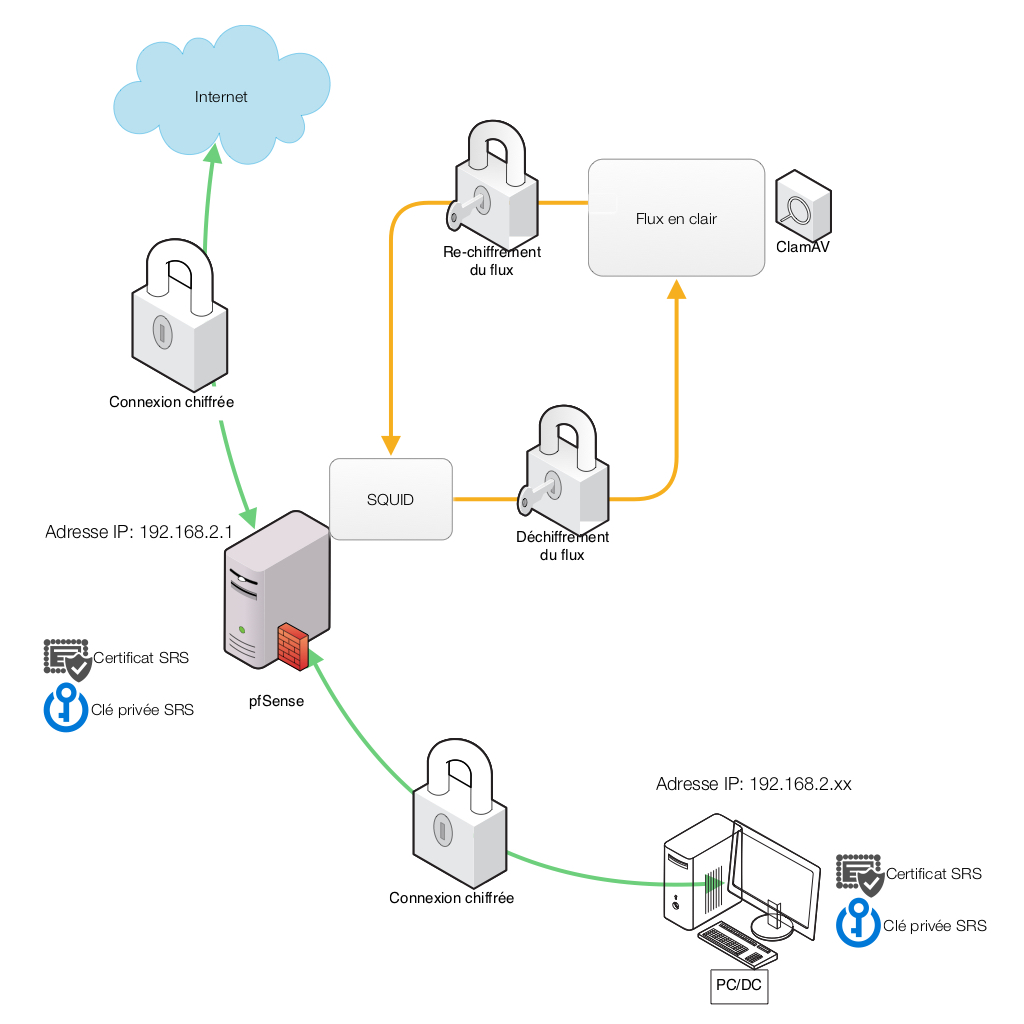
\includegraphics[scale=0.5]{Interception_Screenshots/schema.jpeg}
        \caption{Schéma de l'interception SSL/TLS}
        \label{Schema_tls/1}
    \end{center}
\end{figure}
\FloatBarrier 

\newpage
\subsection{Accès à Pfsense et installation des paquets}
Pour pouvoir obtenir SQUID il faut :
\begin{itemize}
    \item Se connecter à Pfsense via Internet Explorer
    \item Accéder à \textbf{System -> Package Manager} :
\begin{figure}[h!]
    \begin{center}
        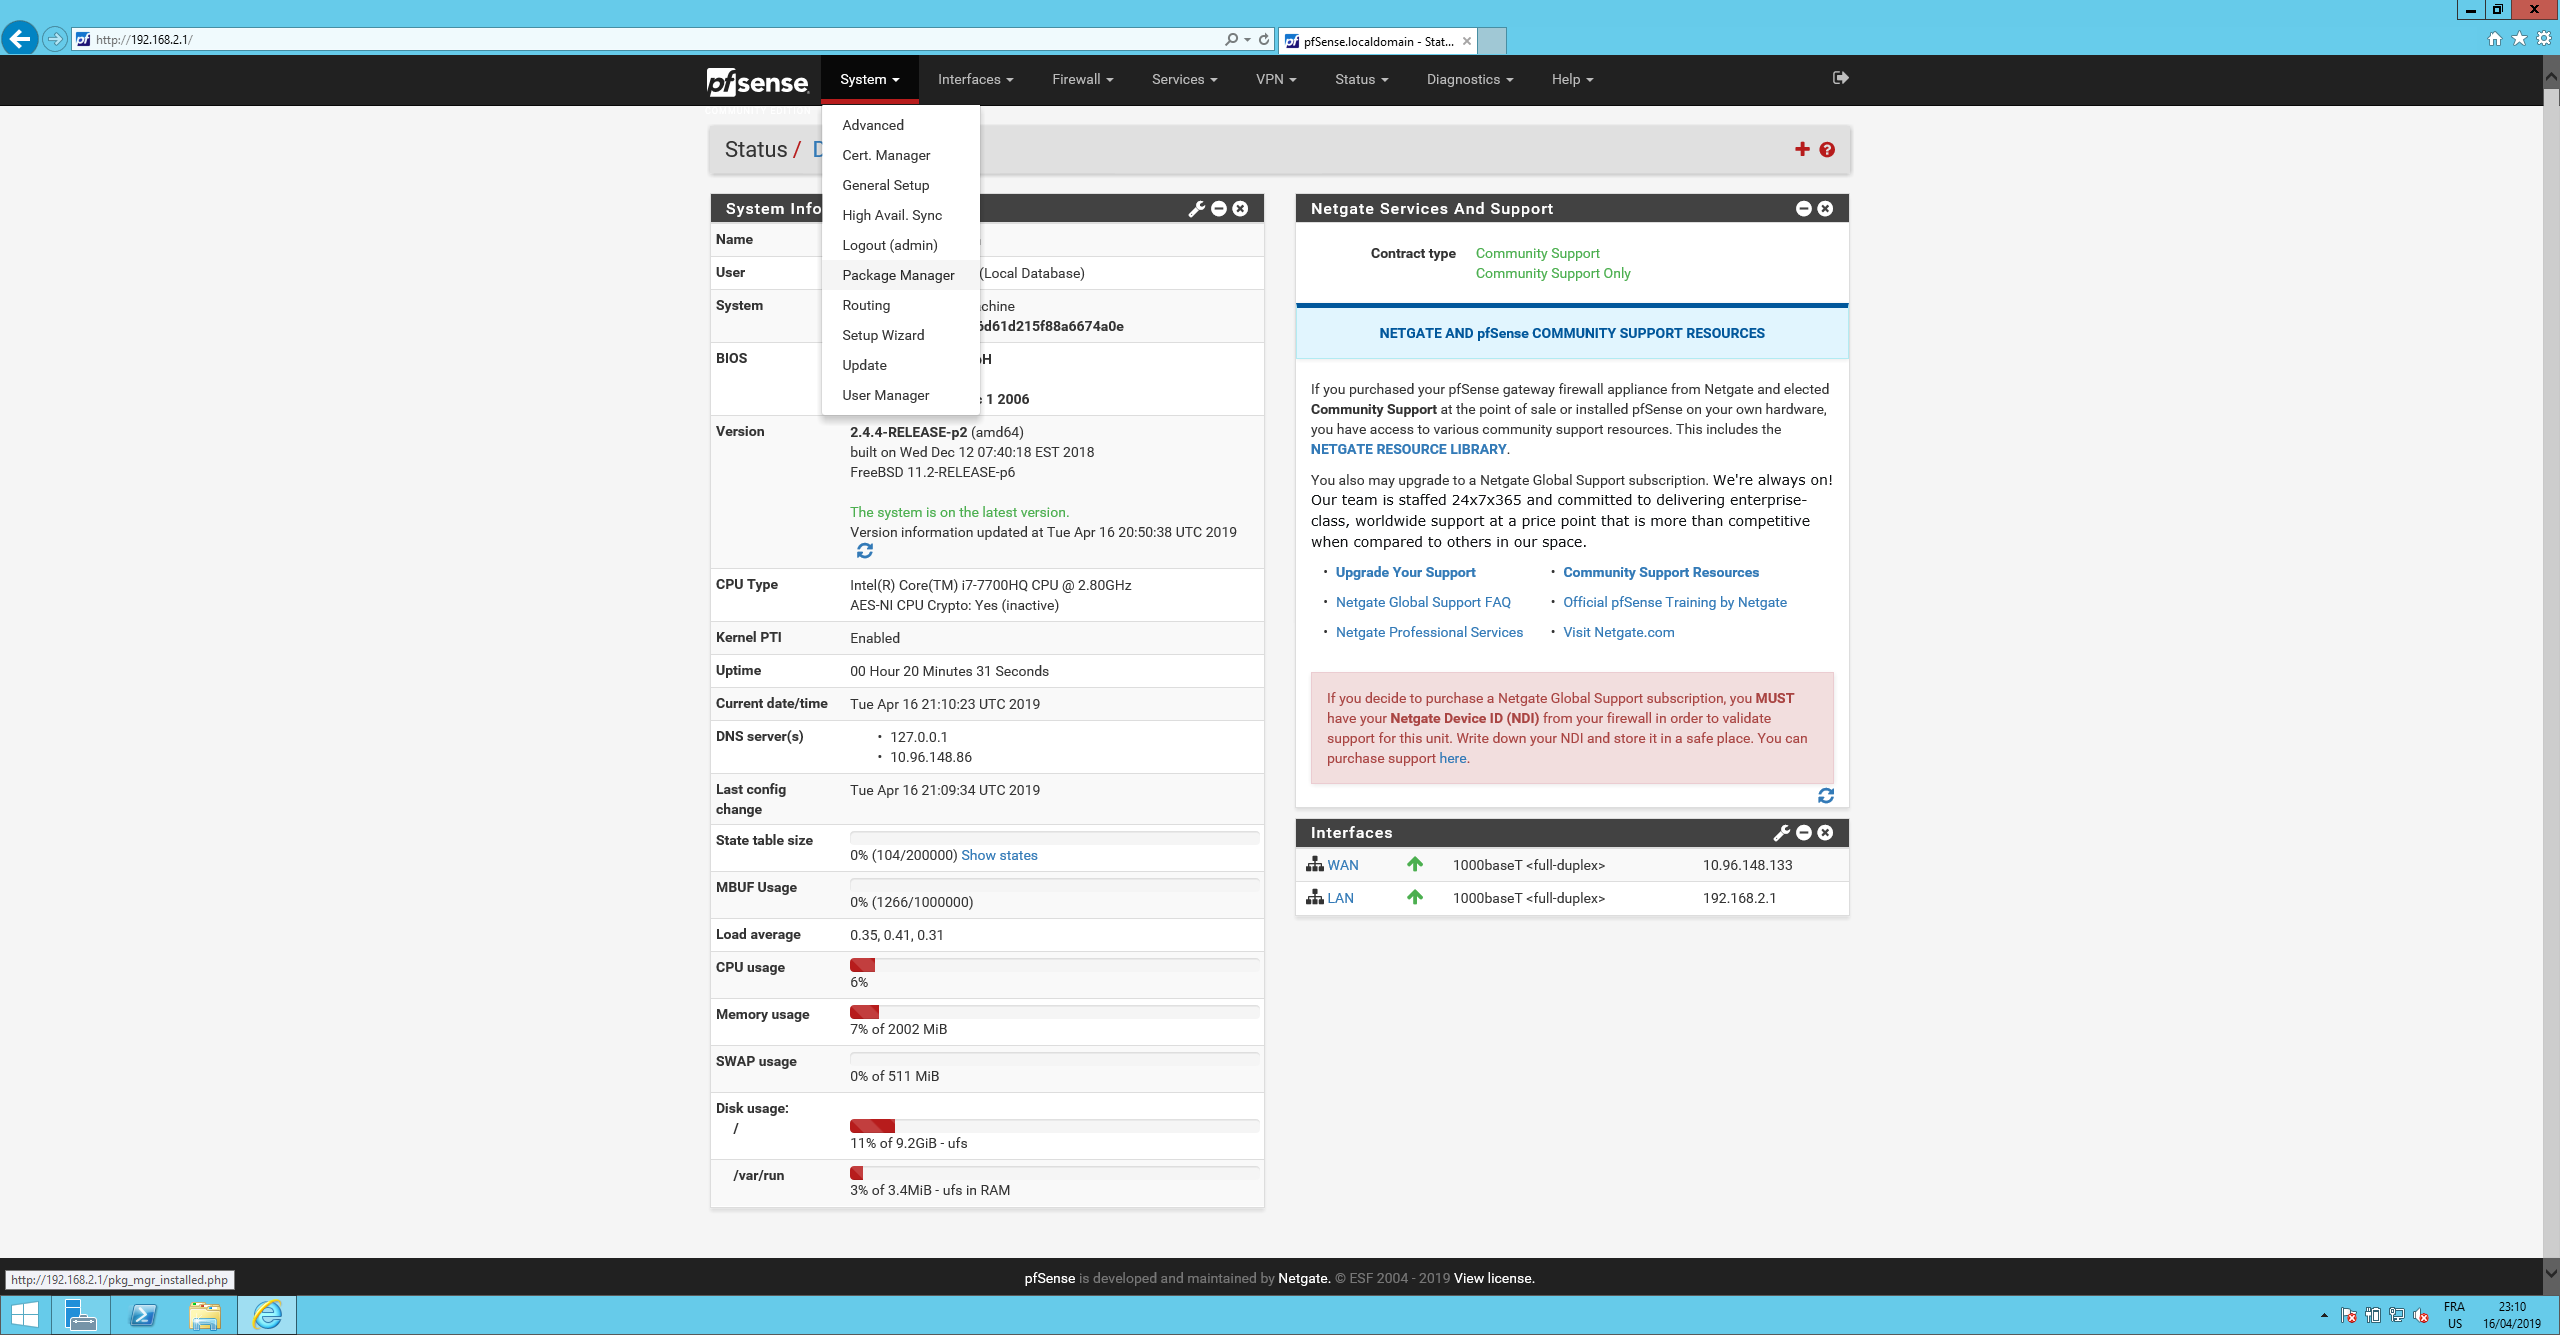
\includegraphics[scale=0.22]{Pfsense_Screeshots/interception/3.png}
        \label{Pfsense_Screeshots/interception/3}
        \caption{Accès au gestionnaire de paquets sur pfsense}
    \end{center}
\end{figure}
\FloatBarrier 

    \item Cliquer sur \textbf{Available Packages} :
\begin{figure}[h!]
    \begin{center}
        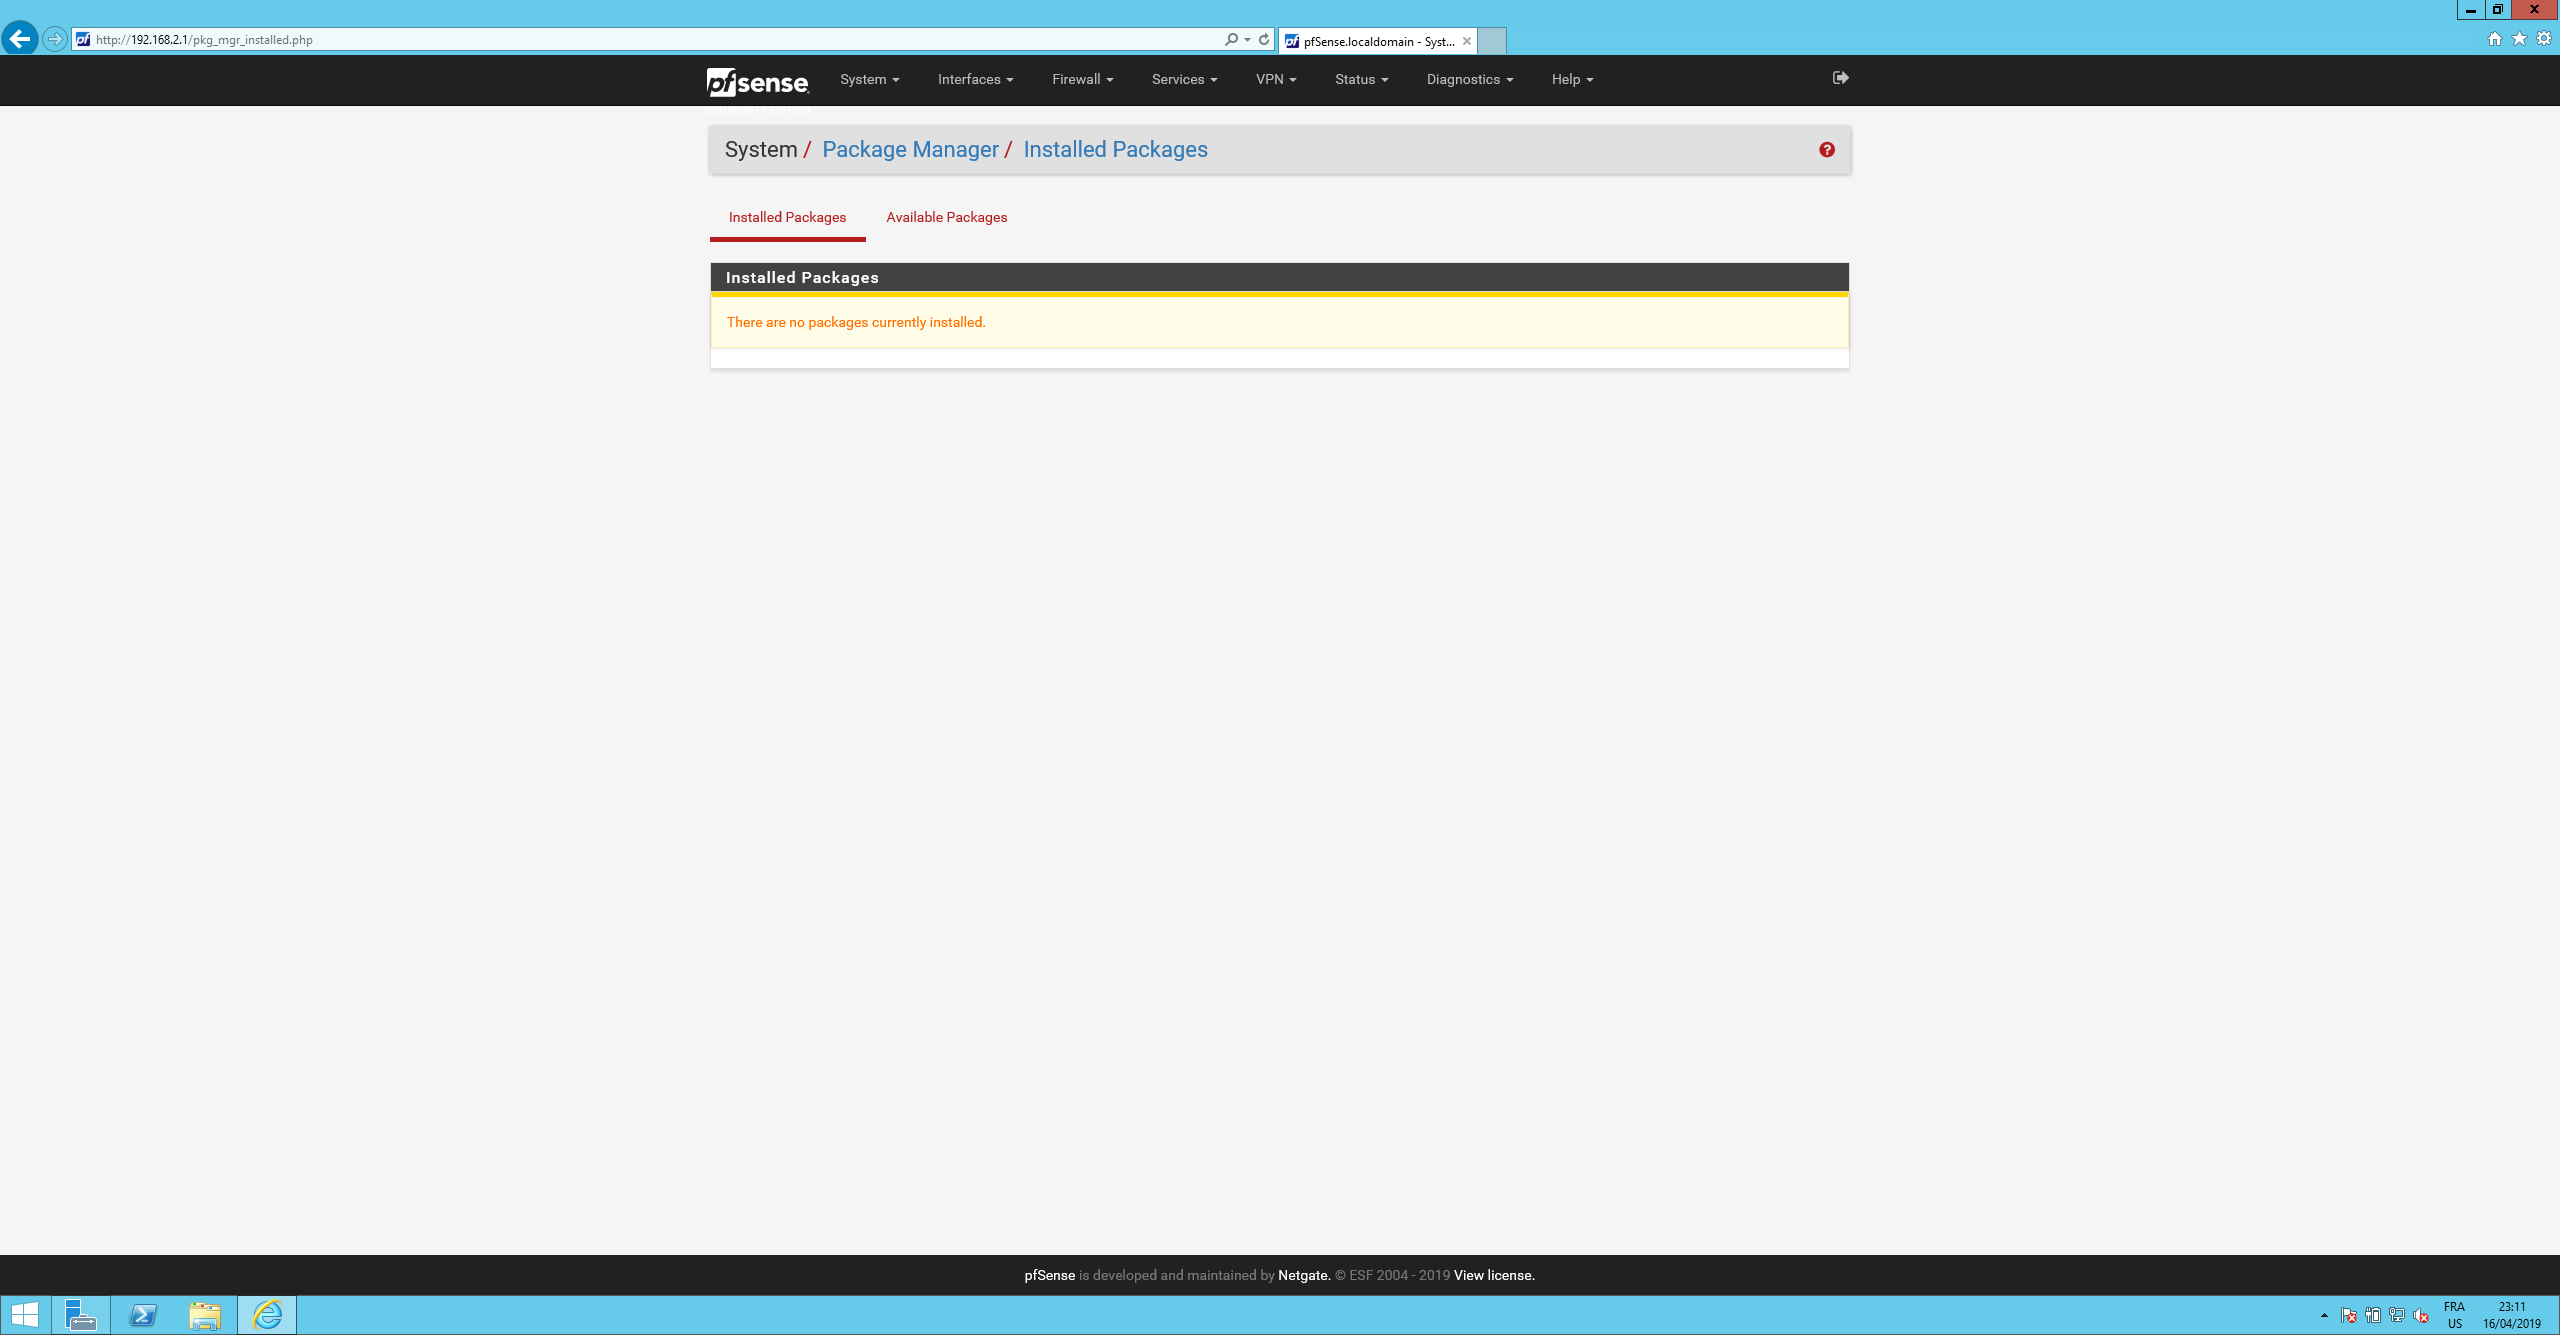
\includegraphics[scale=0.22]{Pfsense_Screeshots/interception/4.png}
        \label{Pfsense_Screeshots/interception/4}
        \caption{Accès à la recherche de paquets sur pfsense}
    \end{center}
\end{figure}
\FloatBarrier 
    
    \item Rechercher \textbf{SQUID} :
\begin{figure}[h!]
    \begin{center}
        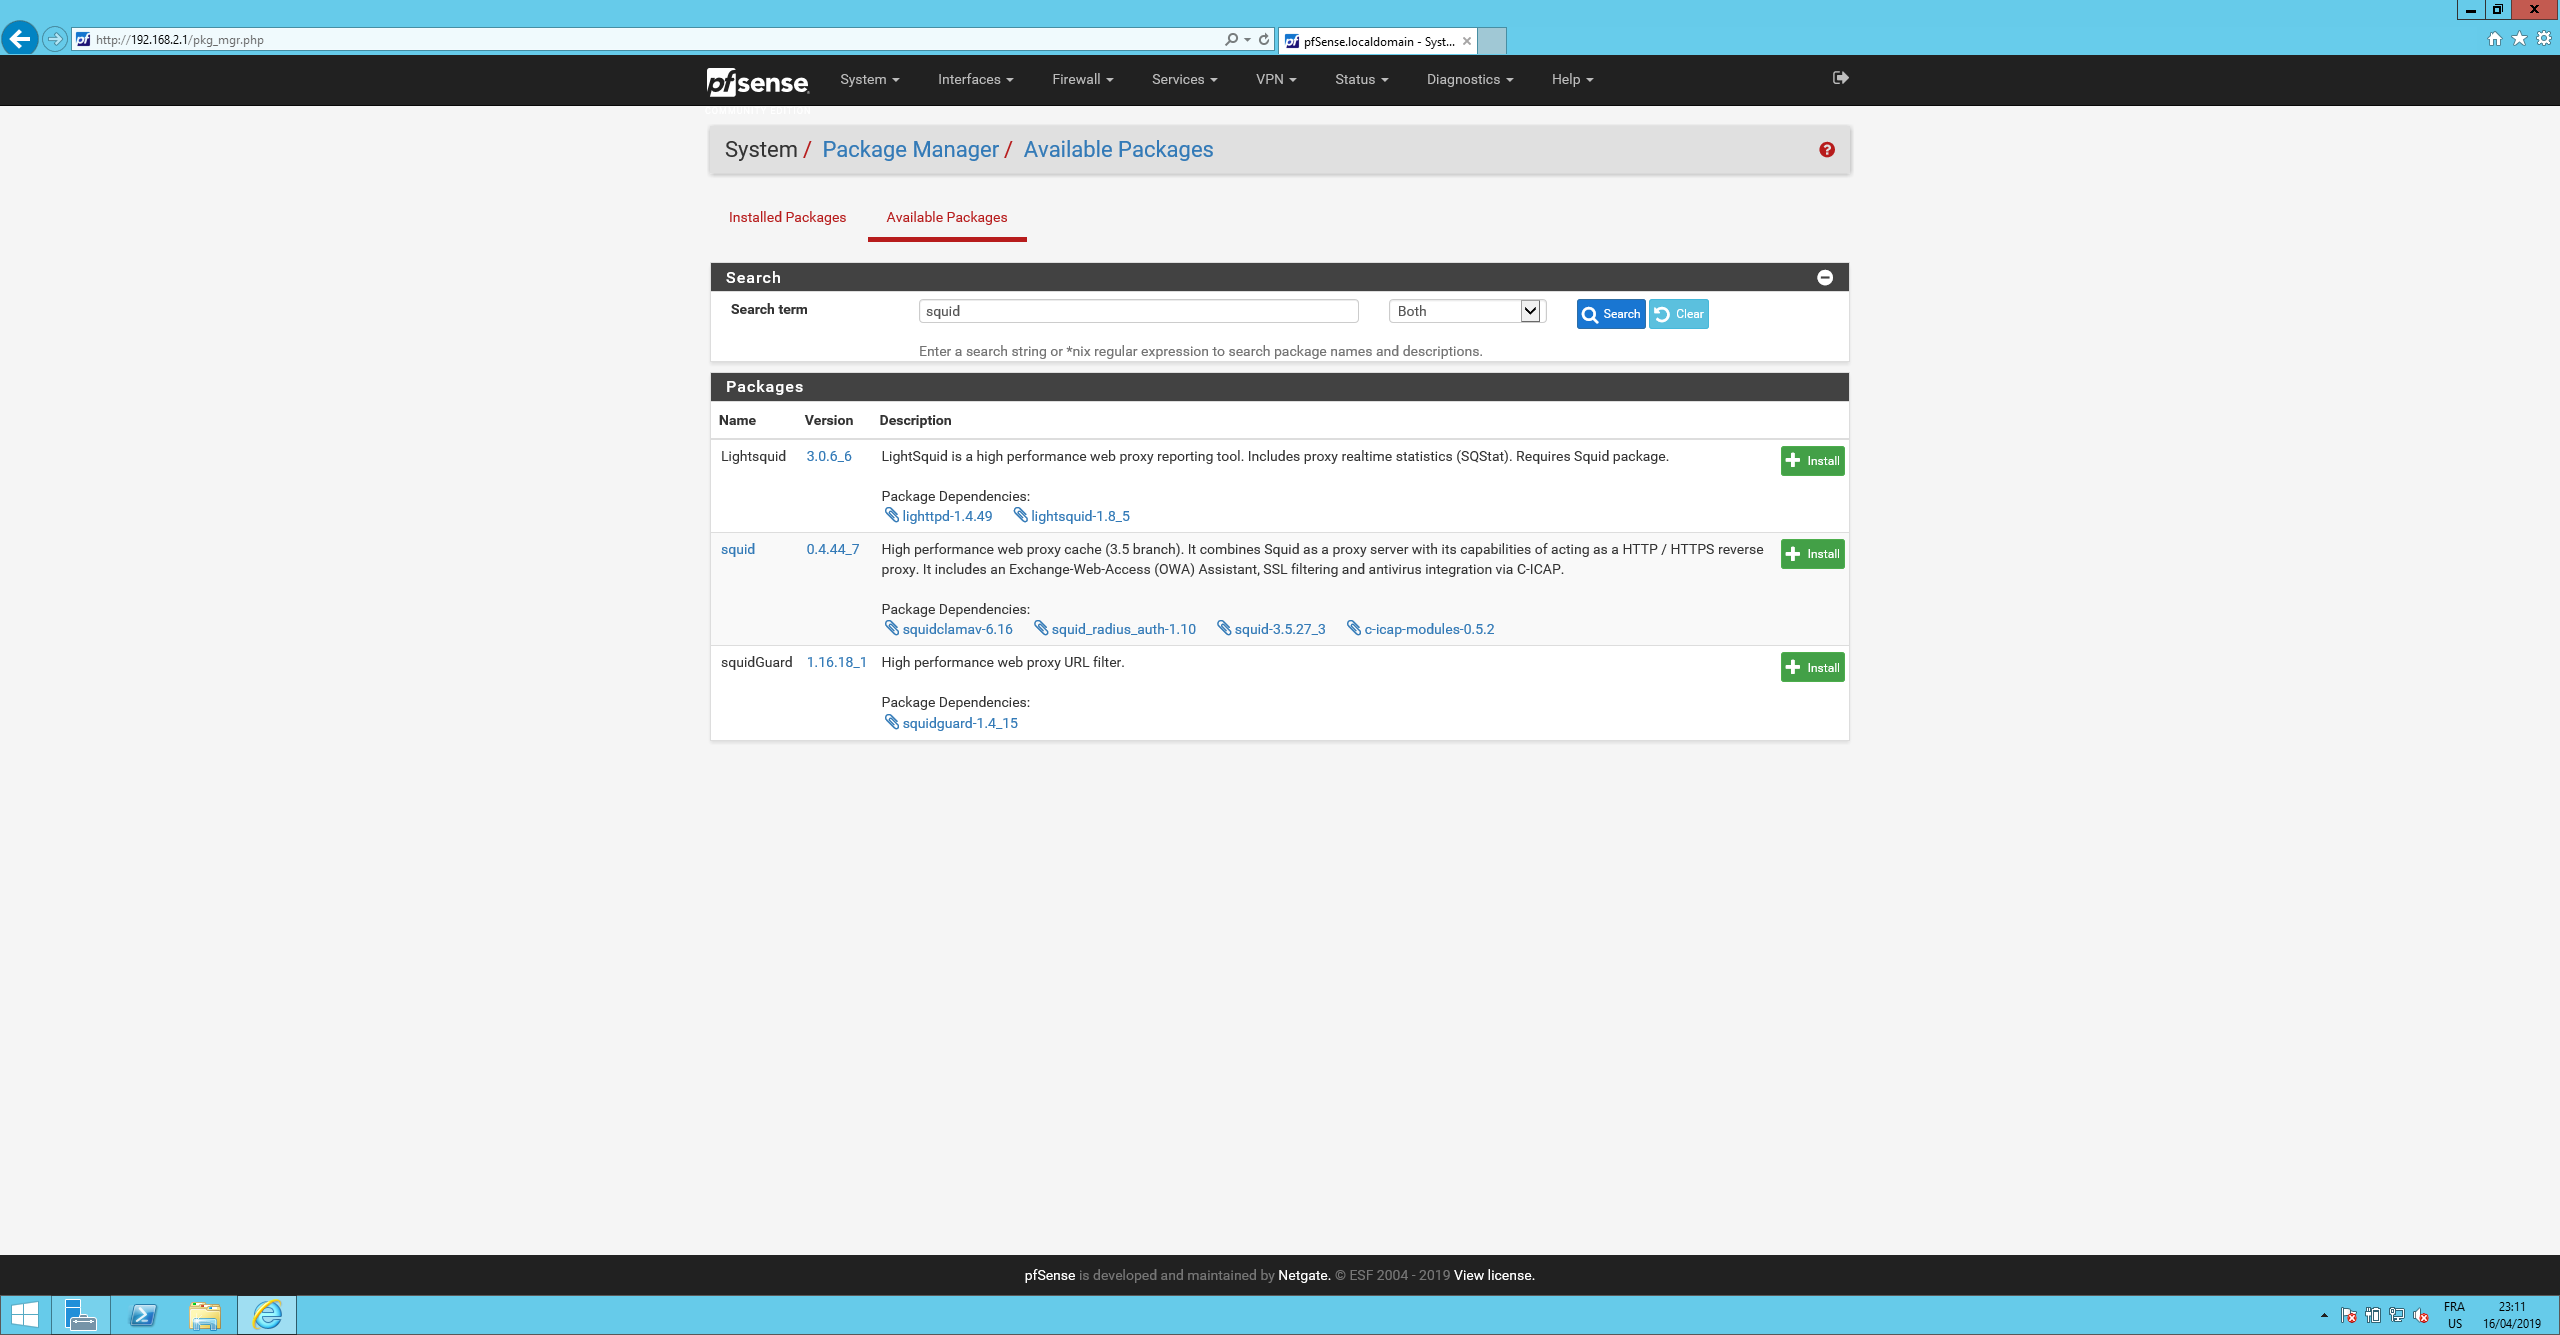
\includegraphics[scale=0.23]{Pfsense_Screeshots/interception/5.png}
        \label{Pfsense_Screeshots/interception/5}
        \caption{Recherche du paquet SQUID sur pfsense}
    \end{center}
\end{figure}
\FloatBarrier 
    
    \item Cliquer sur \textbf{Install}
    \item Cliquer sur \textbf{Confirm} :
\begin{figure}[h!]
    \begin{center}
        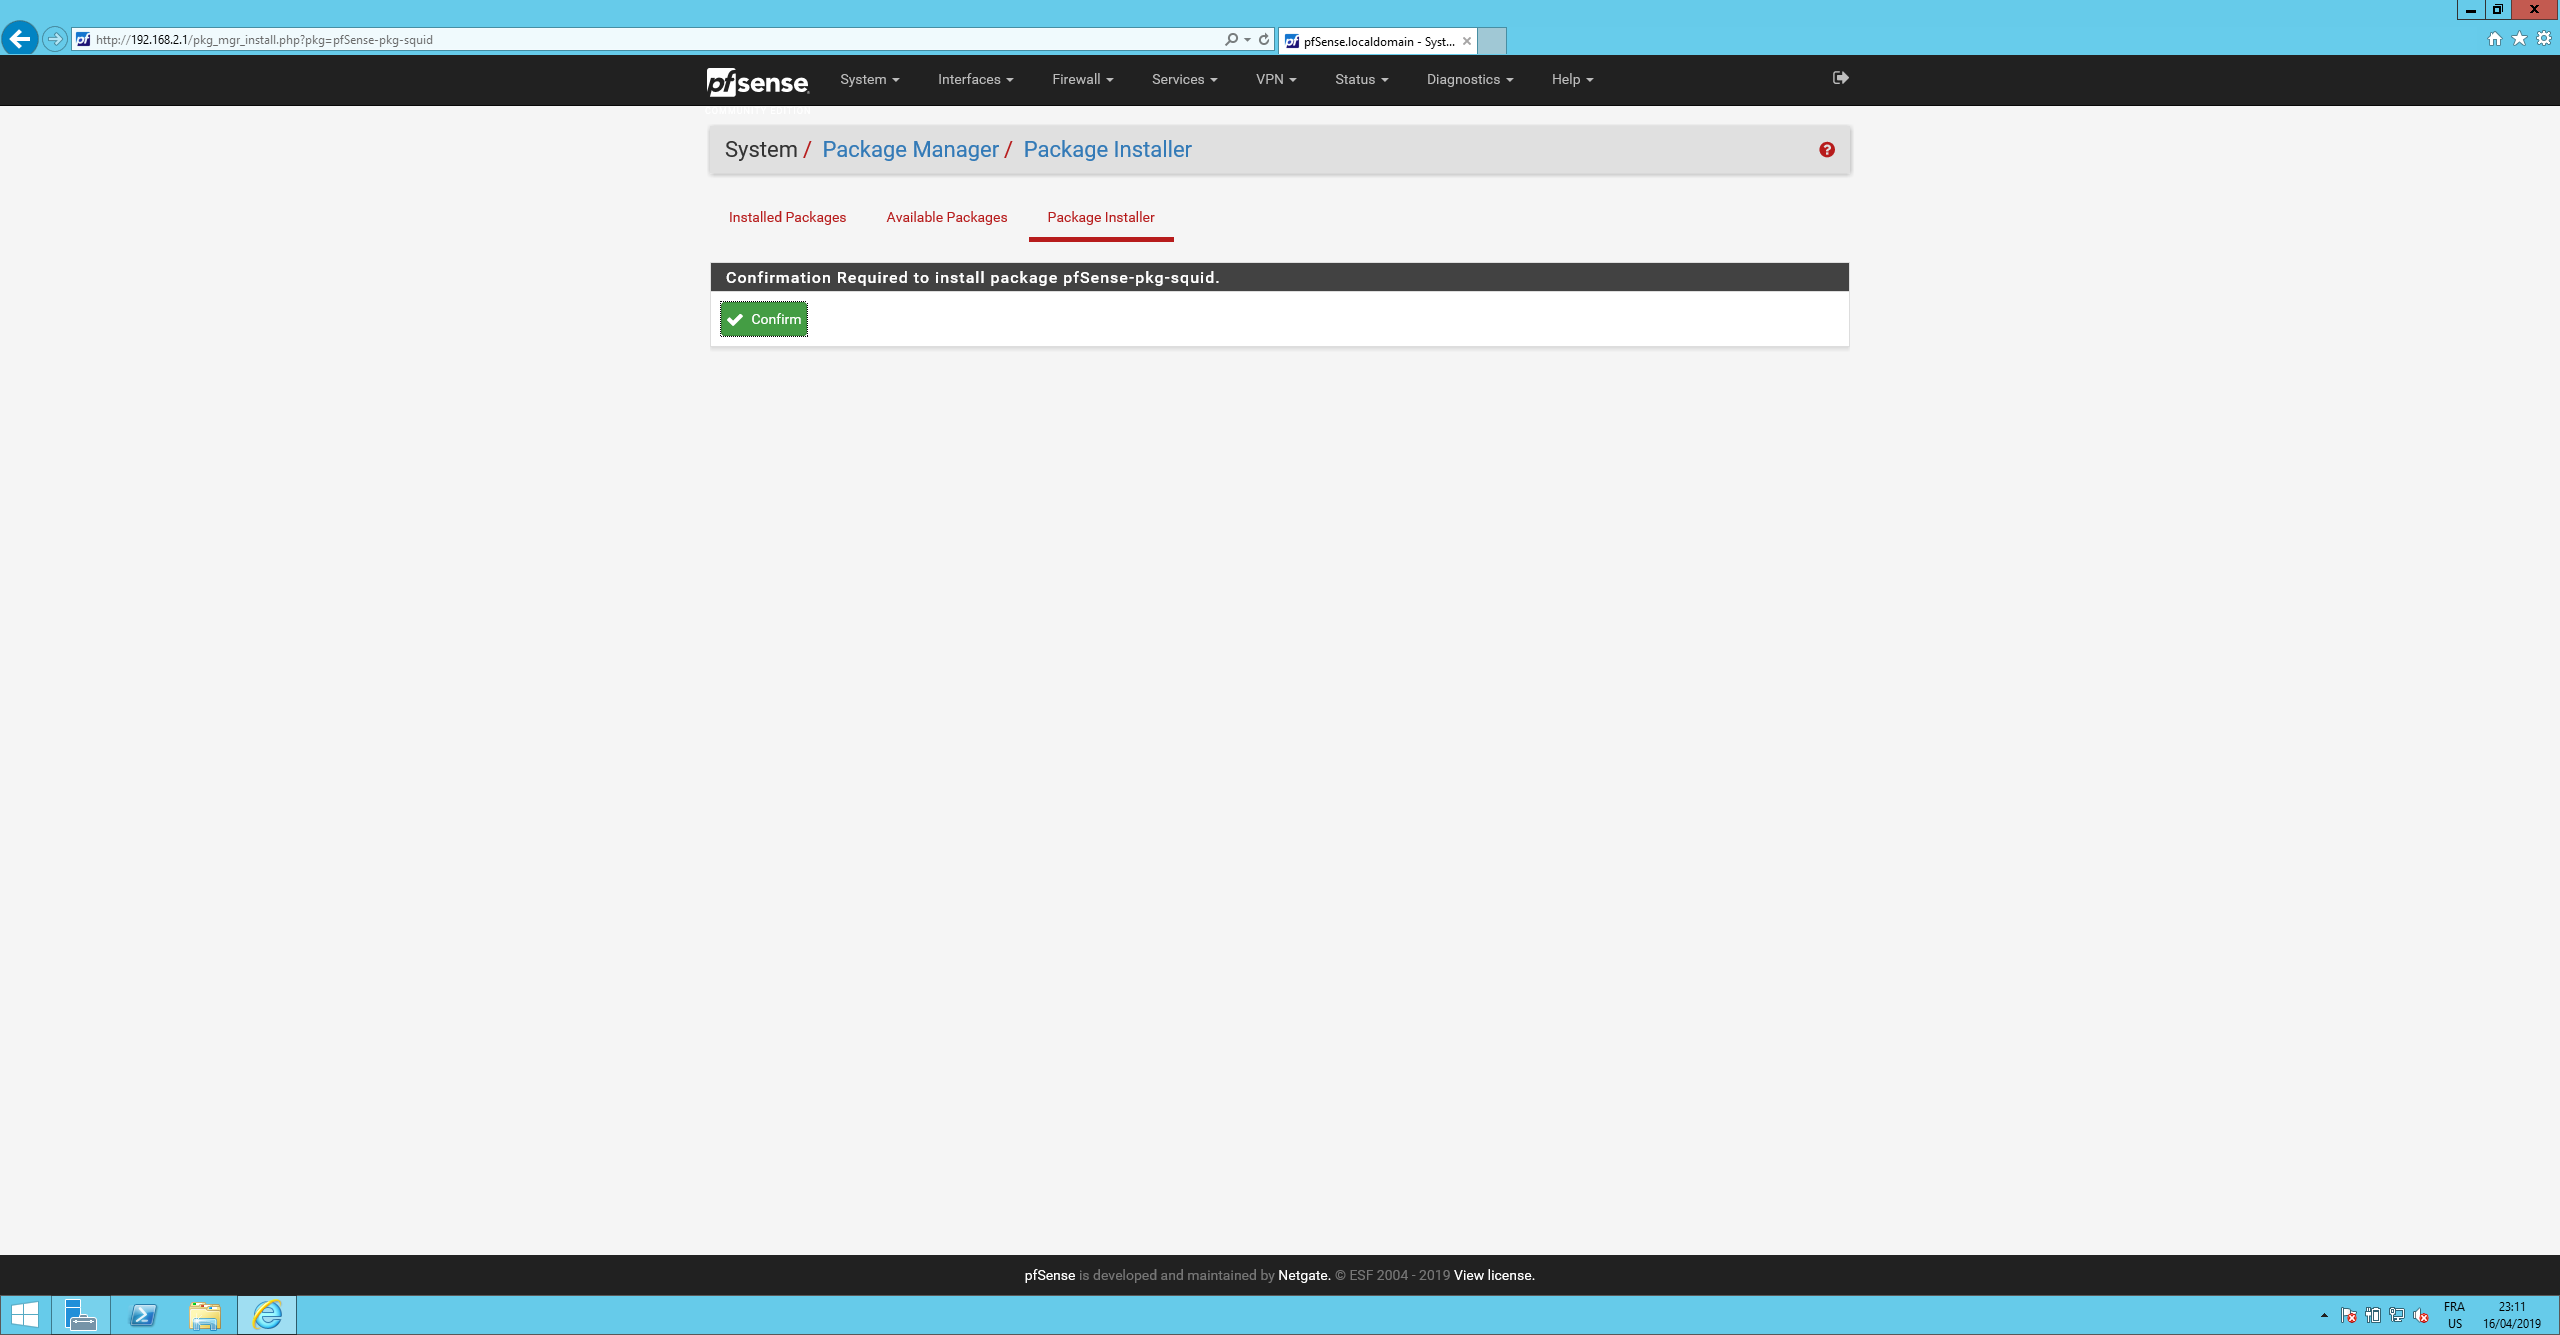
\includegraphics[scale=0.23]{Pfsense_Screeshots/interception/6.png}
        \label{Pfsense_Screeshots/interception/6}
        \caption{Acceptation du paquet à installer sur pfsense}
    \end{center}
\end{figure}
\FloatBarrier 
    
    \item Attendre la fin de l'installation.
\begin{figure}[h!]
    \begin{center}
        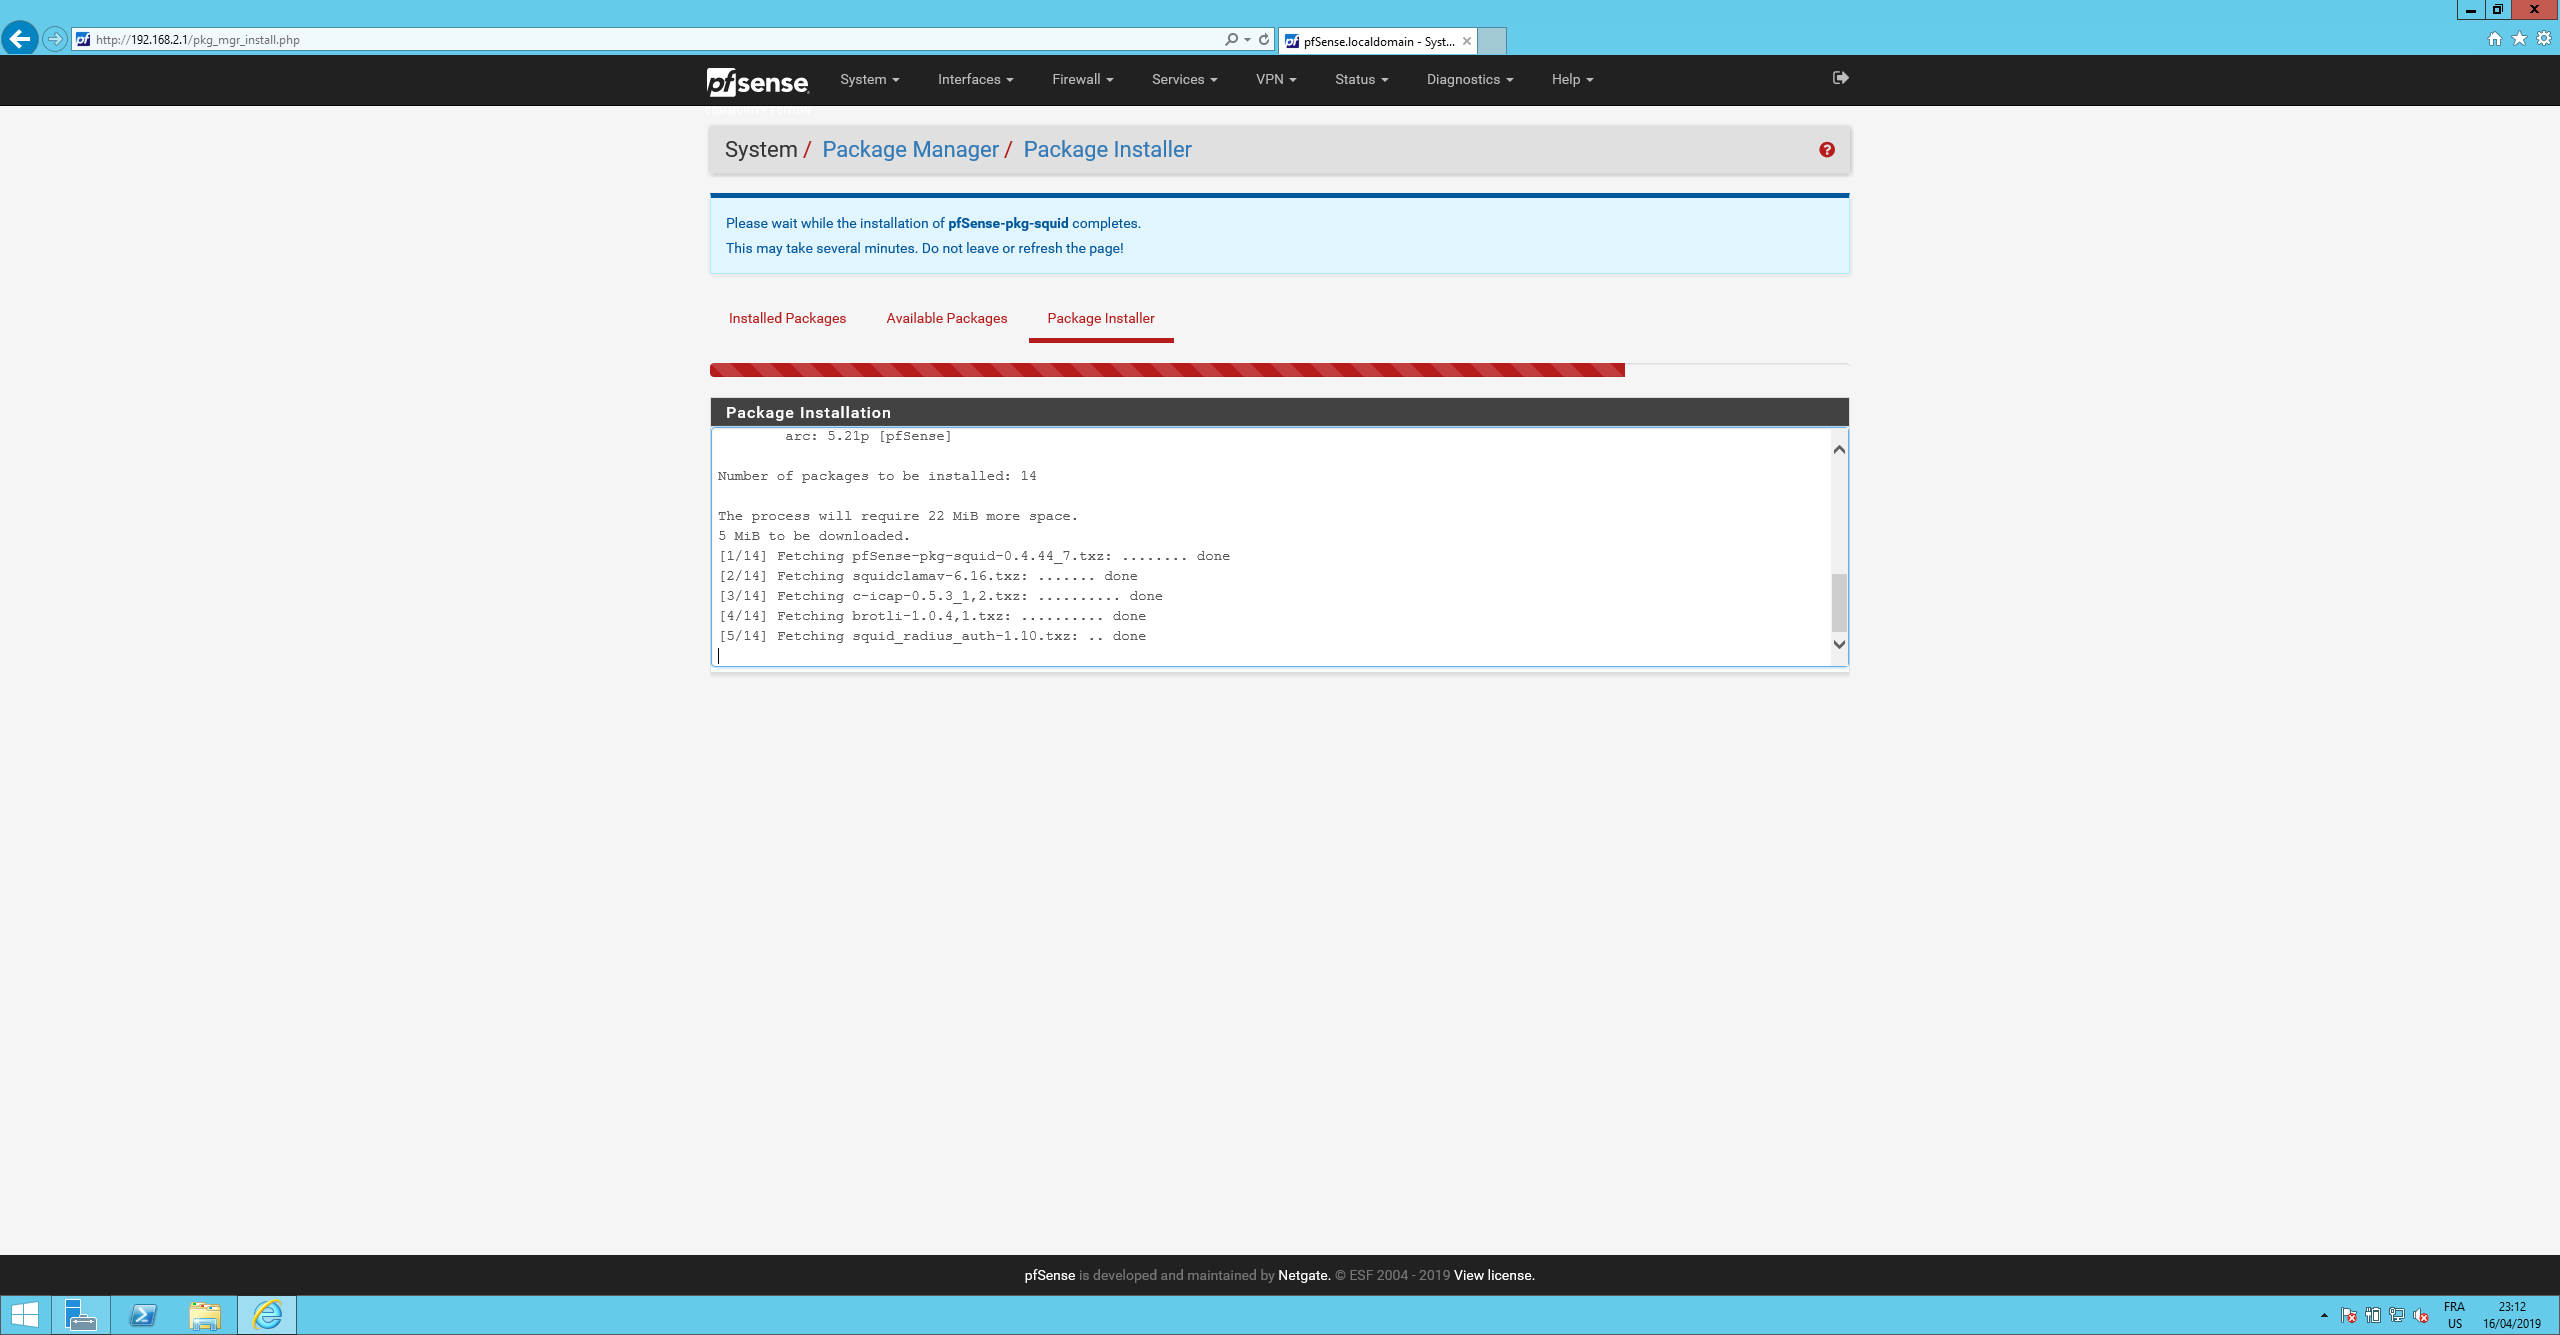
\includegraphics[scale=0.20]{Pfsense_Screeshots/interception/7.png}
        \label{Pfsense_Screeshots/interception/7}
        \caption{Installation en cours du paquet SQUID sur pfsense}
    \end{center}
\end{figure}
\FloatBarrier 
    

\begin{figure}[h!]
    \begin{center}
        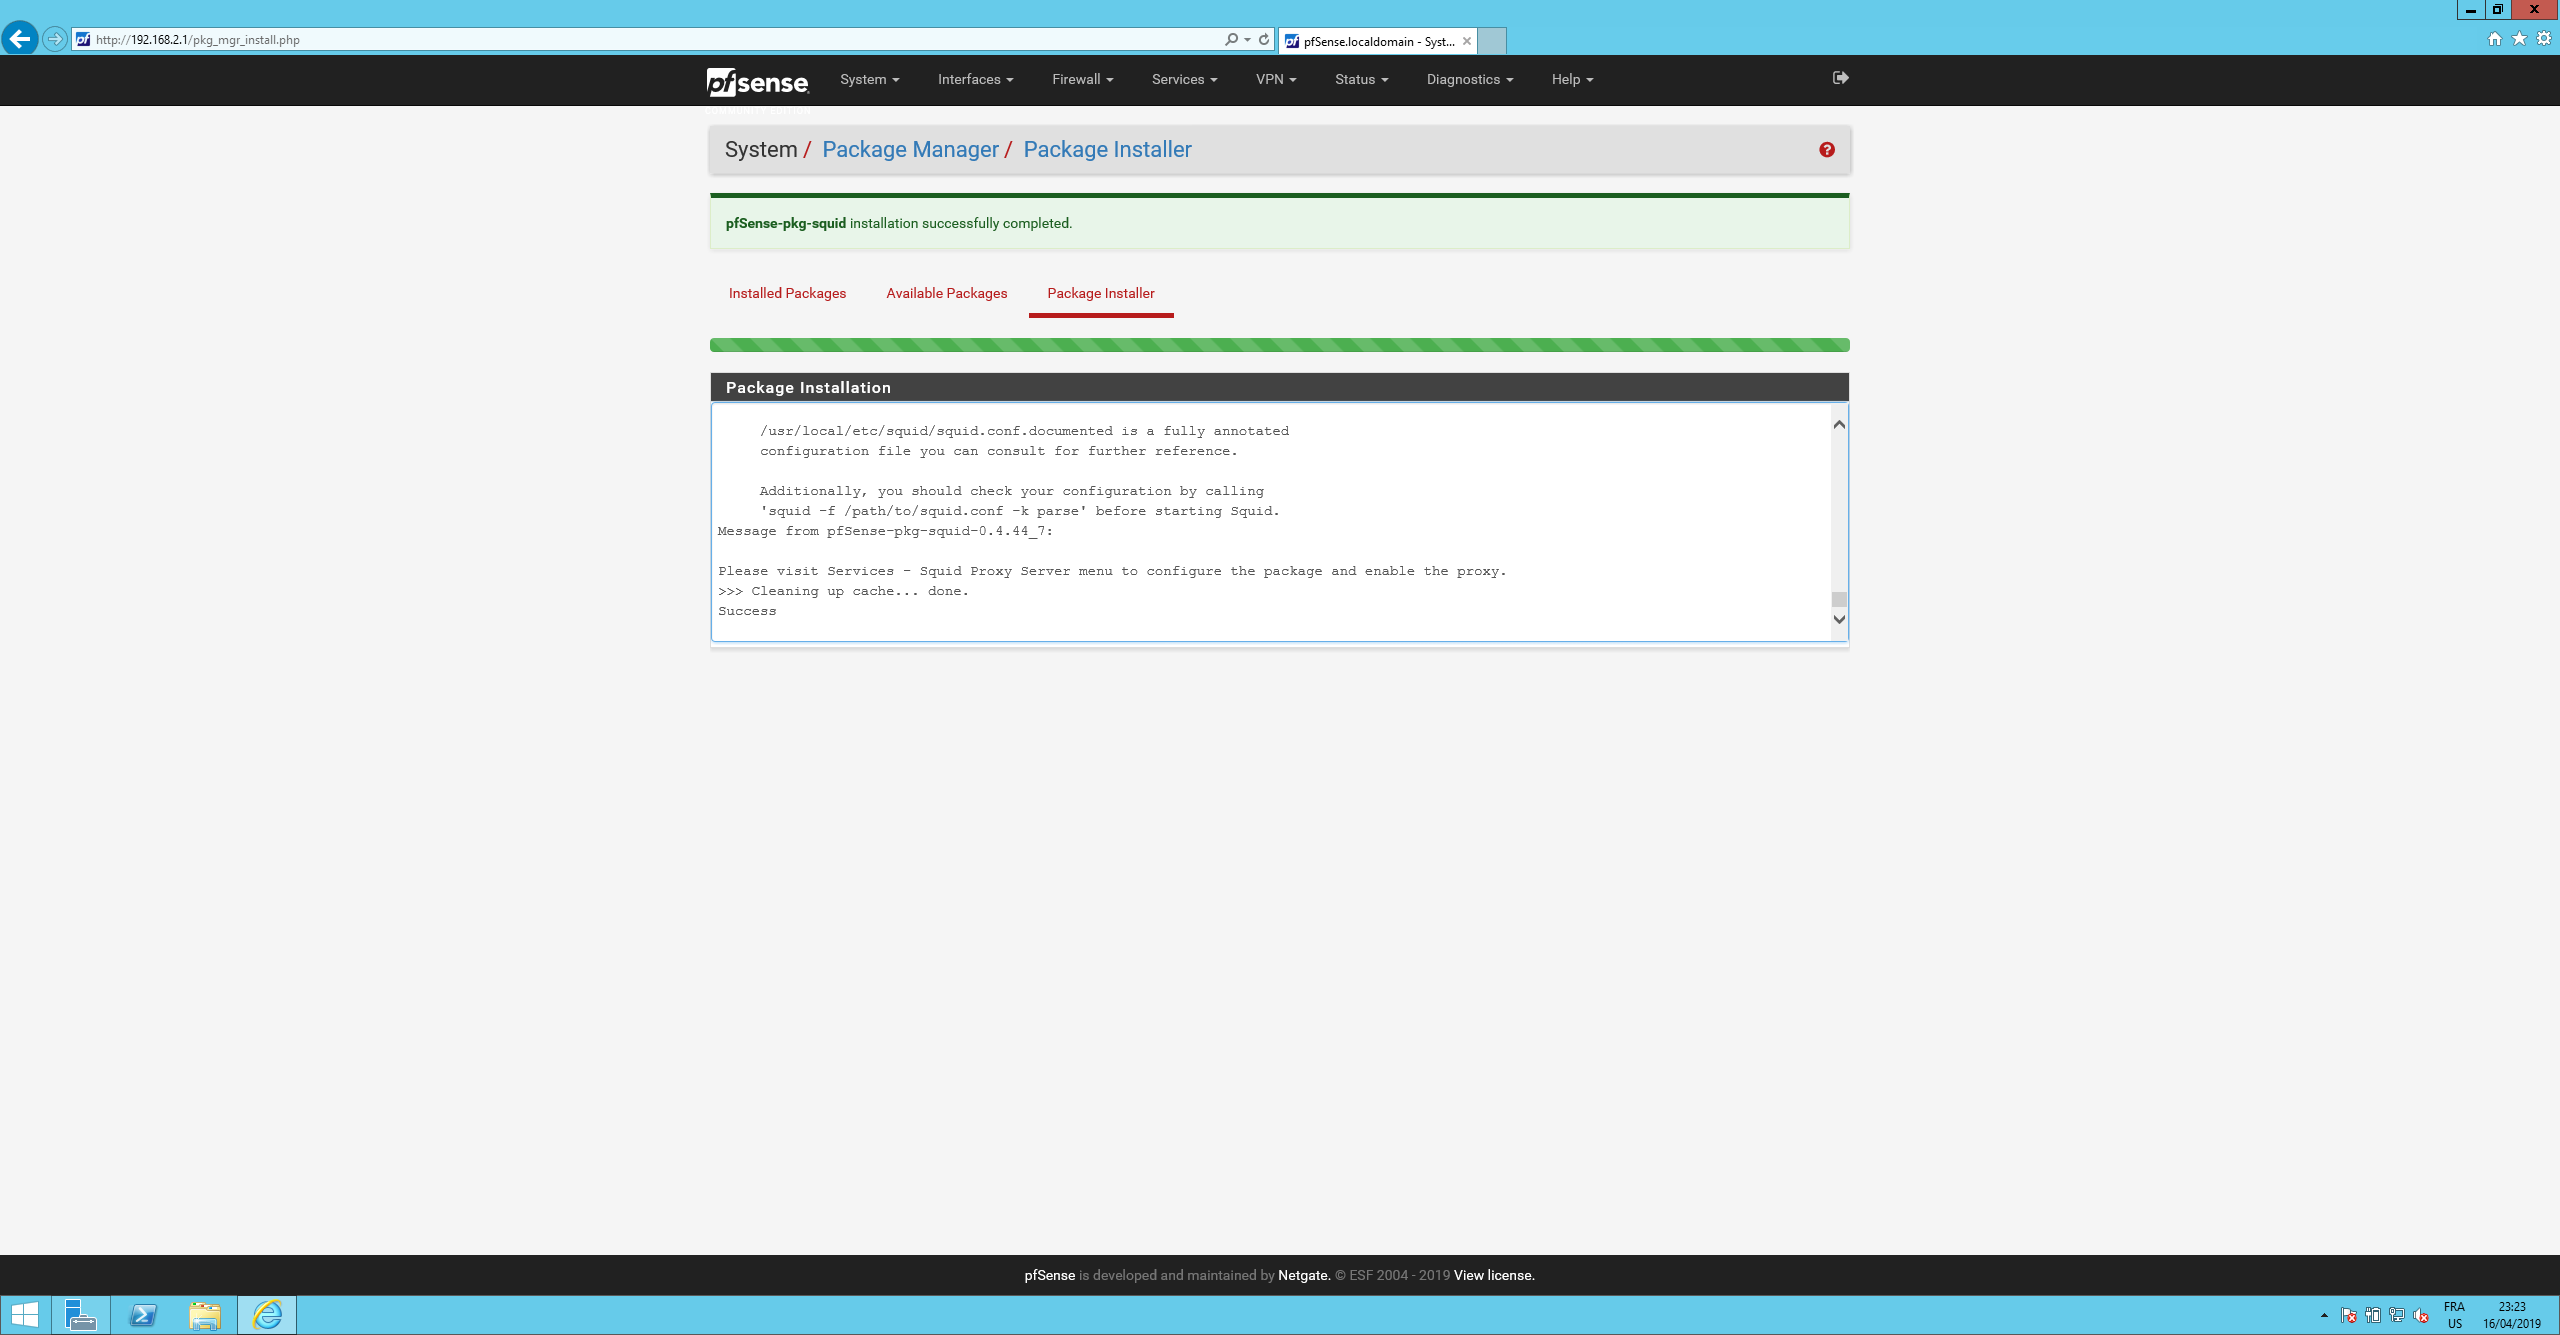
\includegraphics[scale=0.20]{Pfsense_Screeshots/interception/8.png}
        \label{Pfsense_Screeshots/interception/8}
        \caption{Installation terminée de SQUID sur pfsense}
    \end{center}
\end{figure}
\FloatBarrier 

\end{itemize}


\subsection{Ajout d'un certificat}

Pour ajouter un certificat, il faut :
\begin{itemize}
\item accéder à \textbf{System -> Certificat Manager -> CAs} ;

\item cliquer sur \textbf{Add};

\begin{figure}[h!]
    \begin{center}
        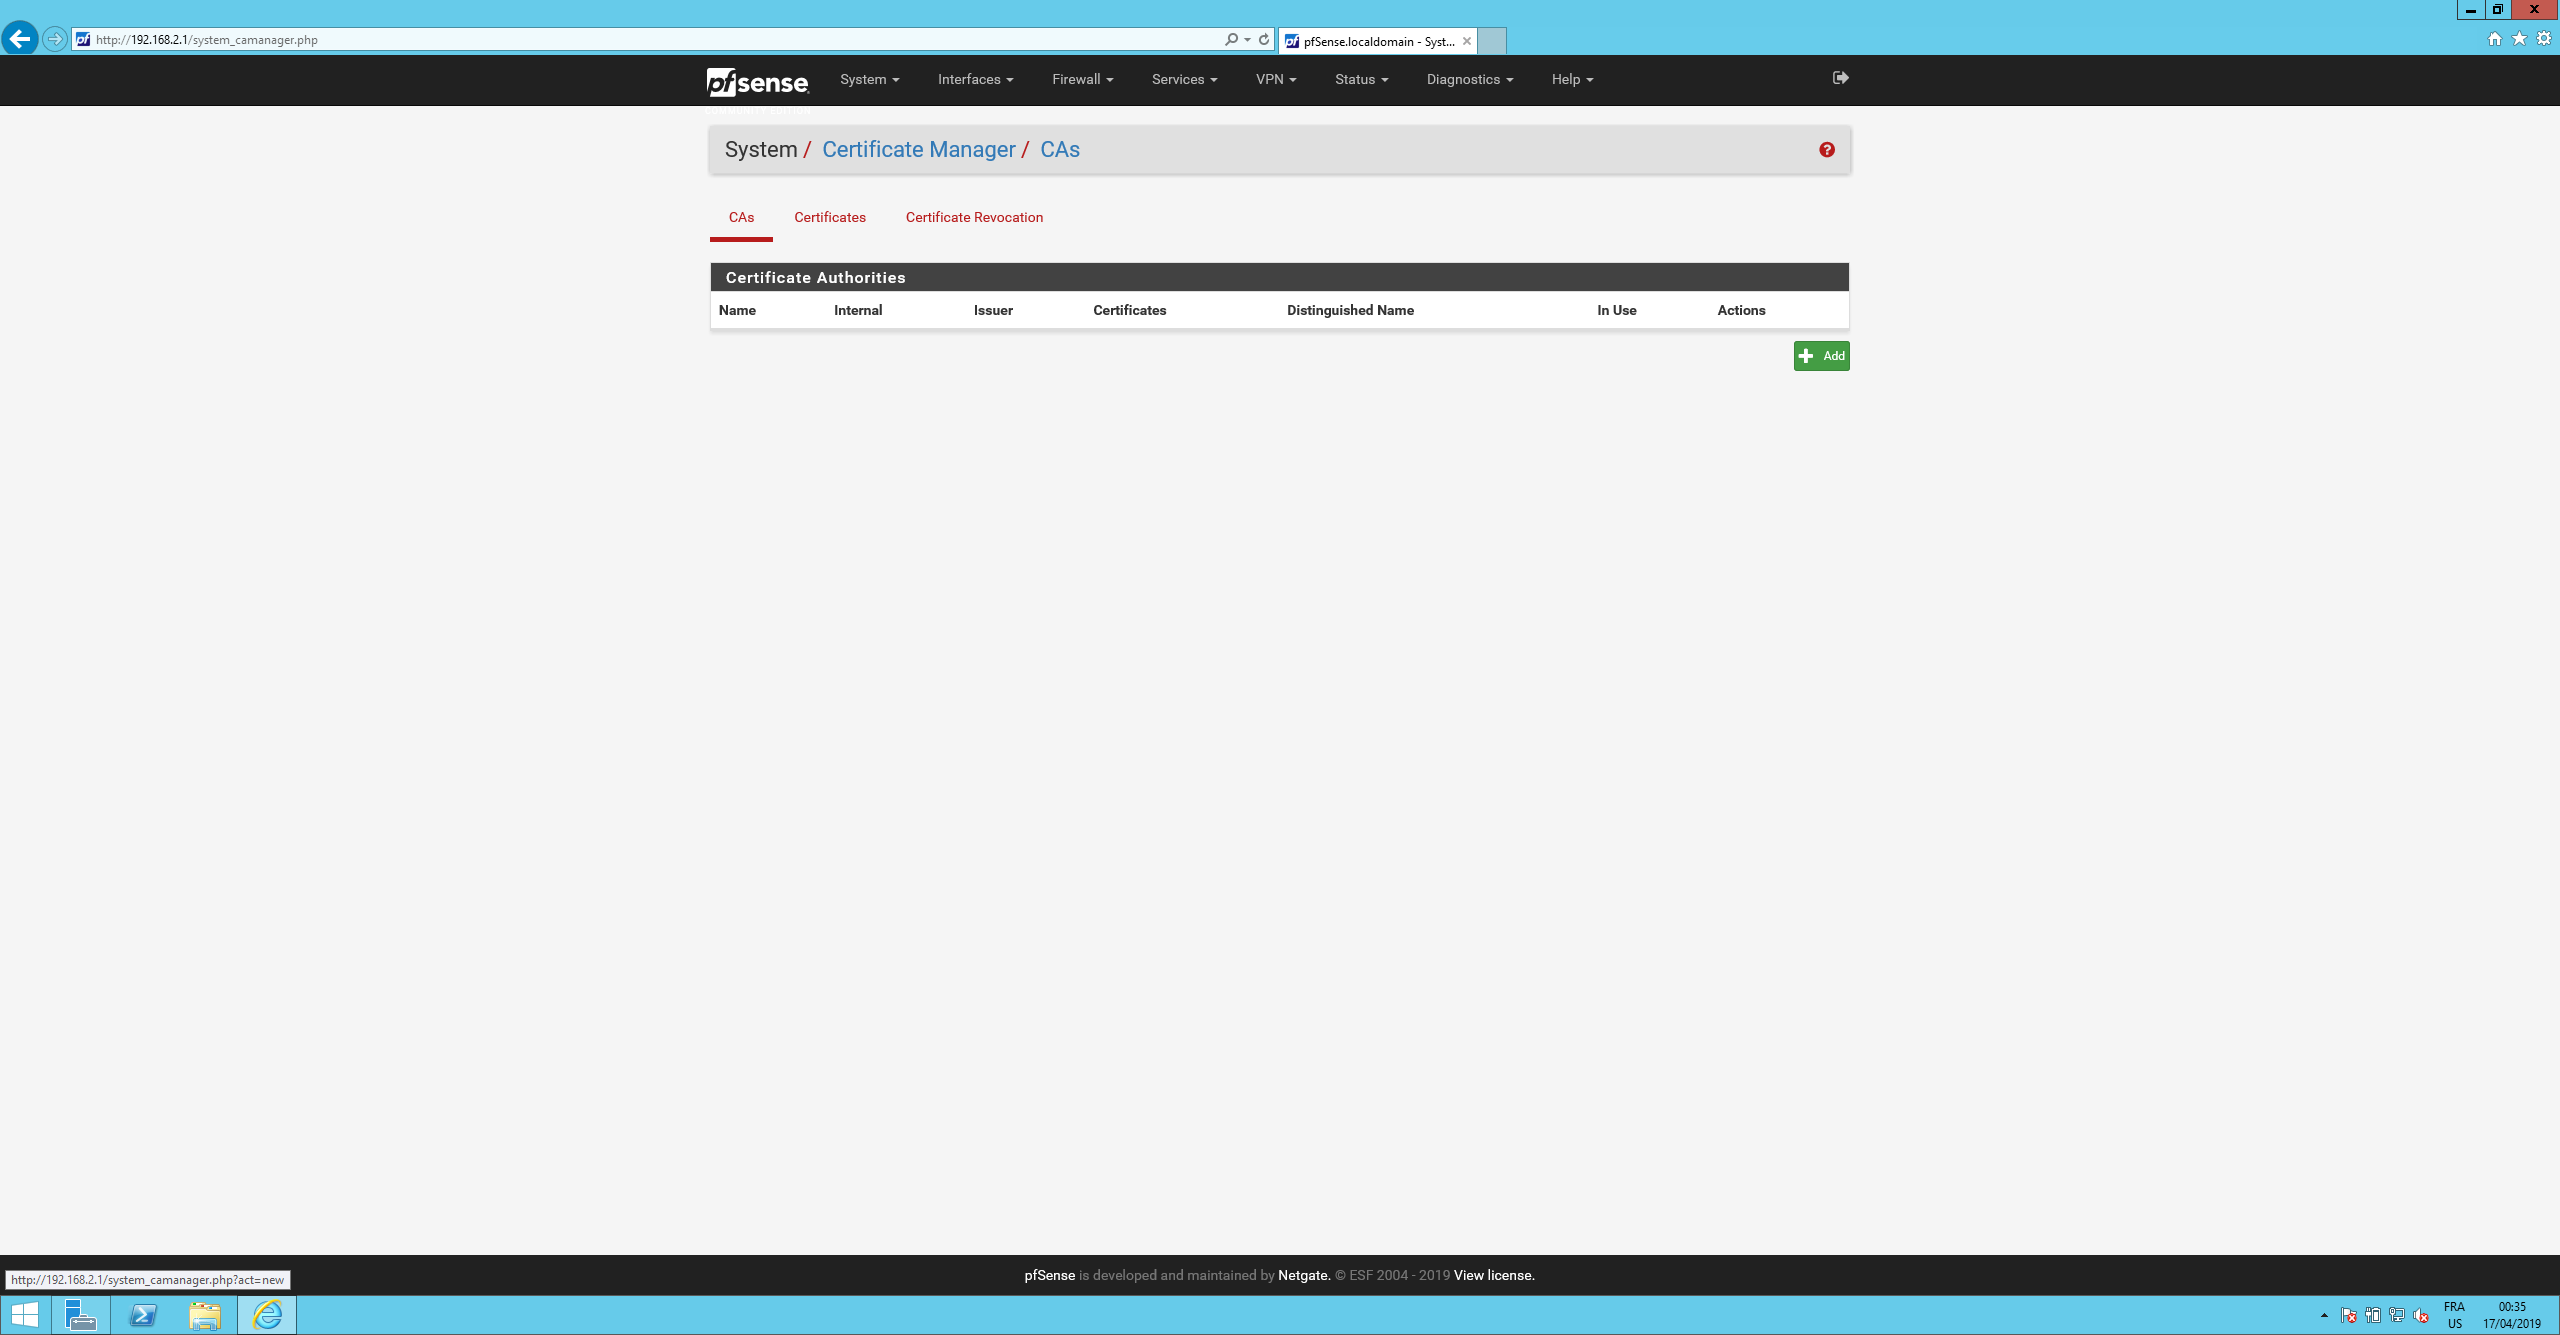
\includegraphics[scale=0.20]{Pfsense_Screeshots/interception/9.png}
        \label{Pfsense_Screeshots/interception/9}
        \caption{Création d'un nouveau certificat sur pfsense}
    \end{center}
\end{figure}
\FloatBarrier 
    
\item renseigner les champs comme ci-dessous :
\begin{figure}[h!]
    \begin{center}
        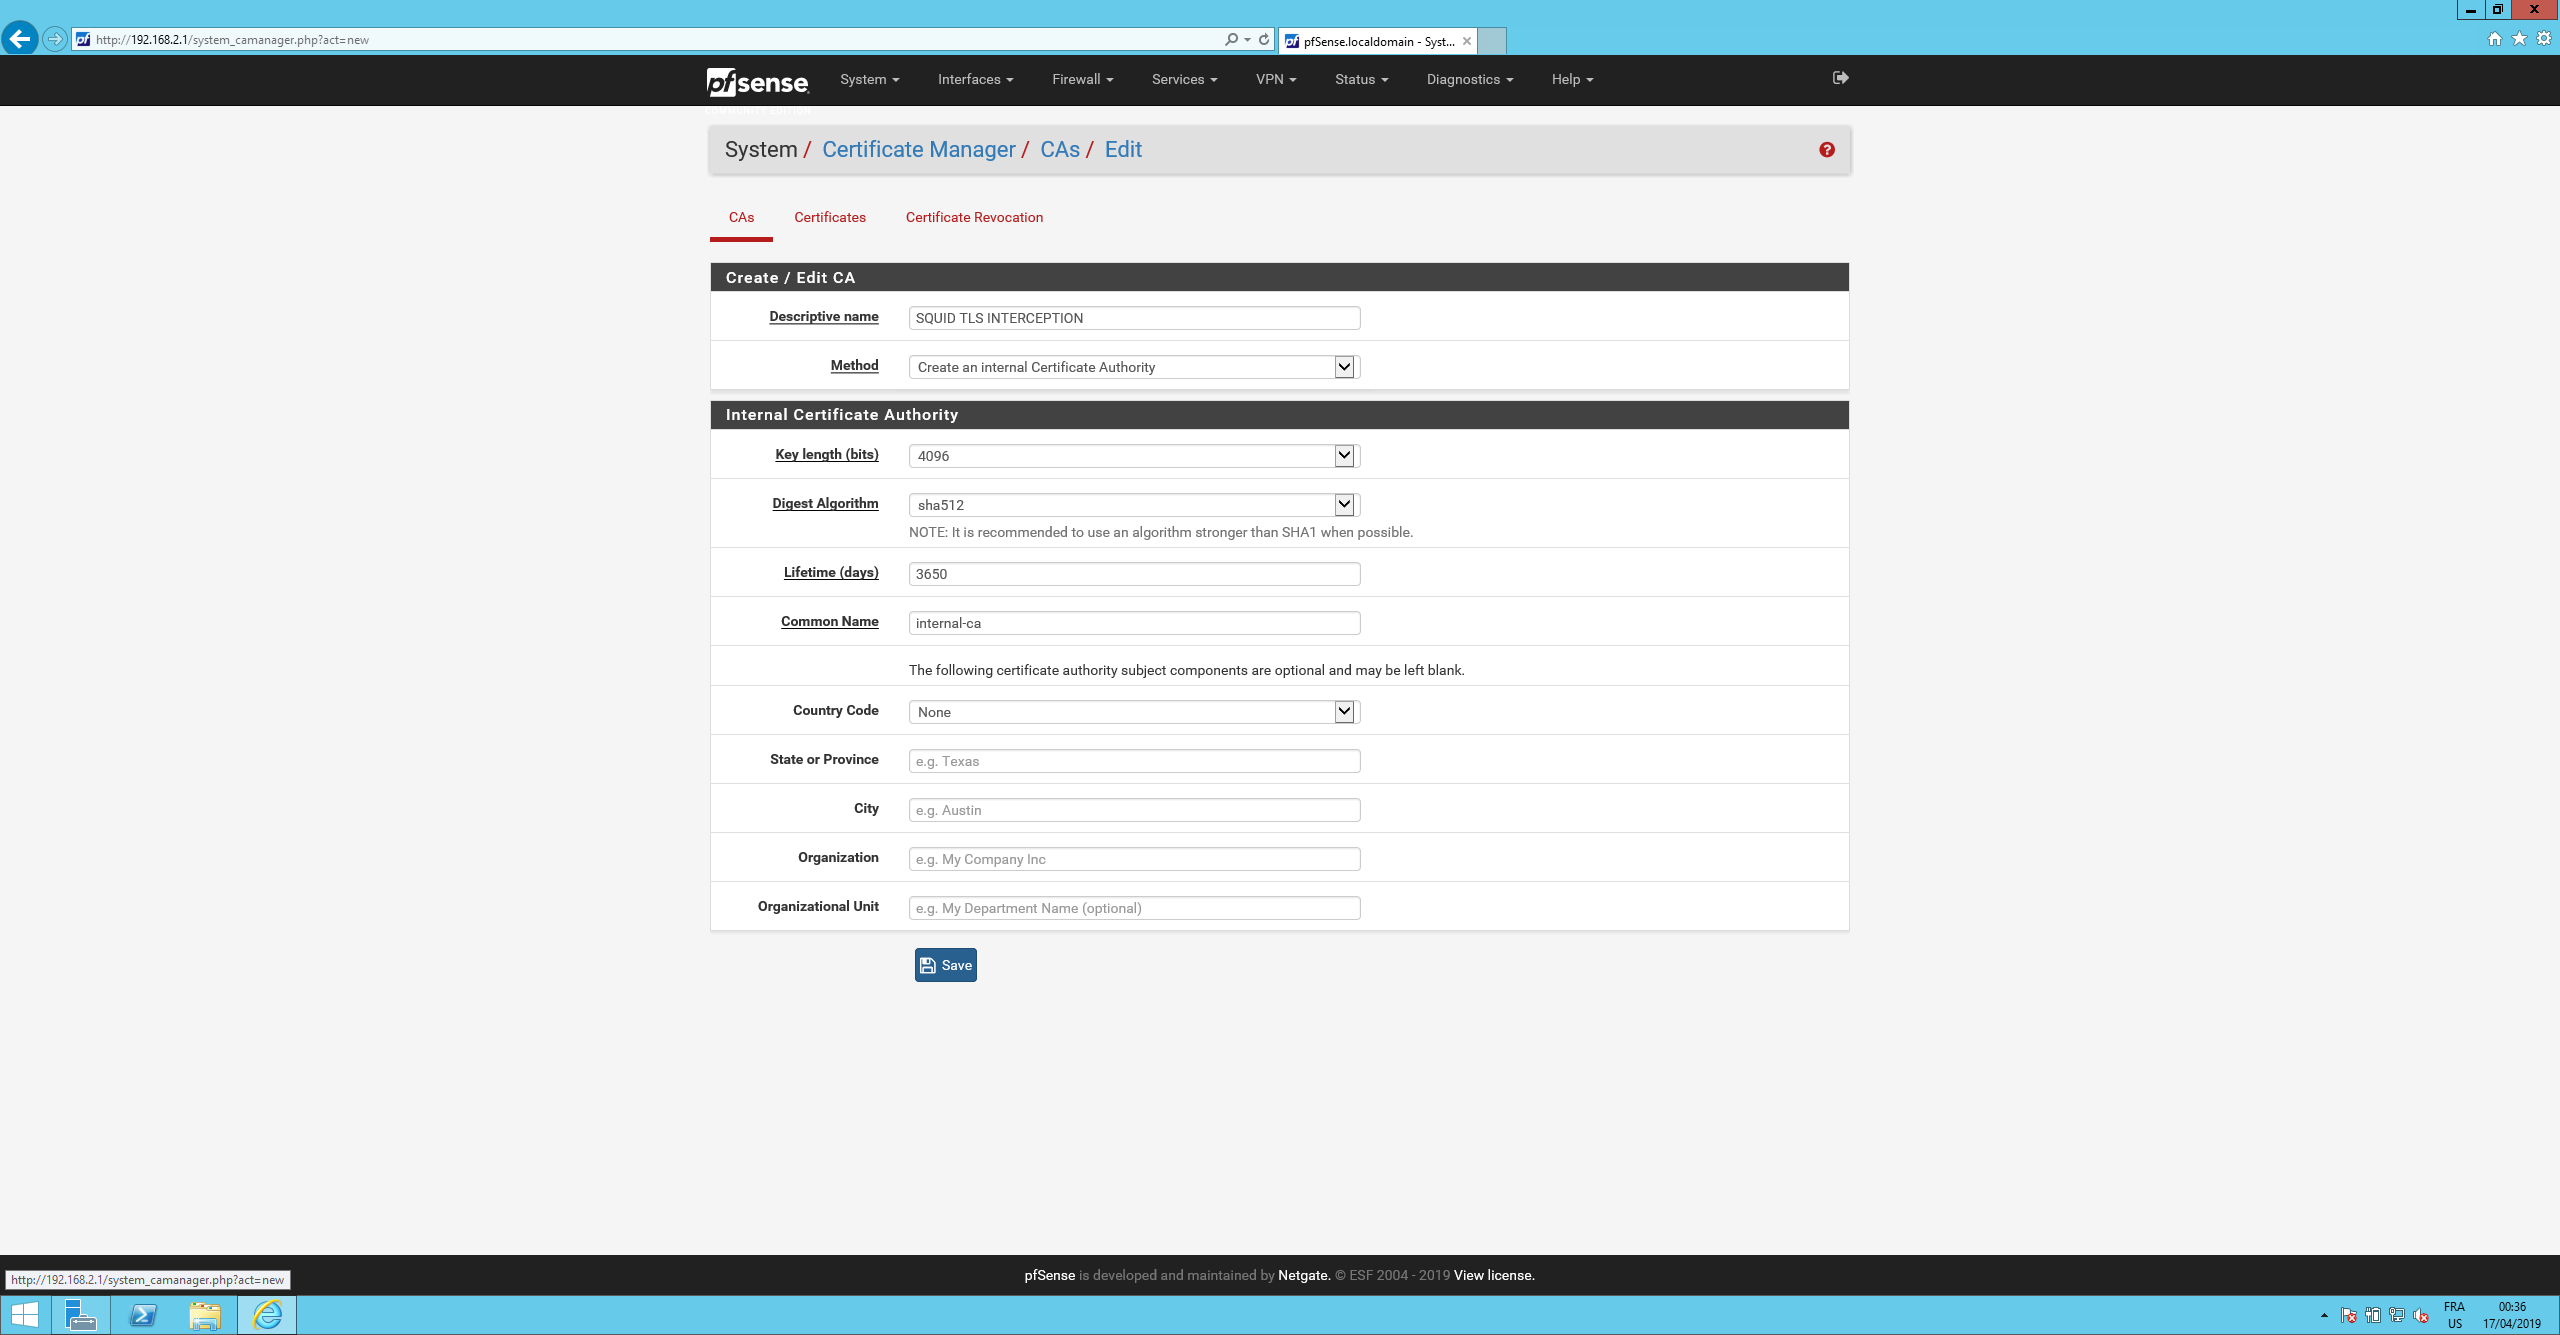
\includegraphics[scale=0.20]{Pfsense_Screeshots/interception/10.png}
        \label{Pfsense_Screeshots/interception/10}
        \caption{Initialisation du nouveau certificat sur pfsense}
    \end{center}
\end{figure}
\FloatBarrier 
\newpage
\end{itemize}
\subsection{Ajout du certificat sur tous les postes appartenant à EPITAF via GPO}
Afin d'intercepter tous les flux provonant du réseau couvert par le domaine EPITAF, voici comment propager le certificat CA à tous les membres du domaine EPITAF :
\begin{itemize}
    \item Depuis le tableau de bord, cliquer sur \textbf{Outils} puis cliquer sur \textbf{Gestion des politiques de groupe} ;
\begin{figure}[h!]
    \begin{center}
        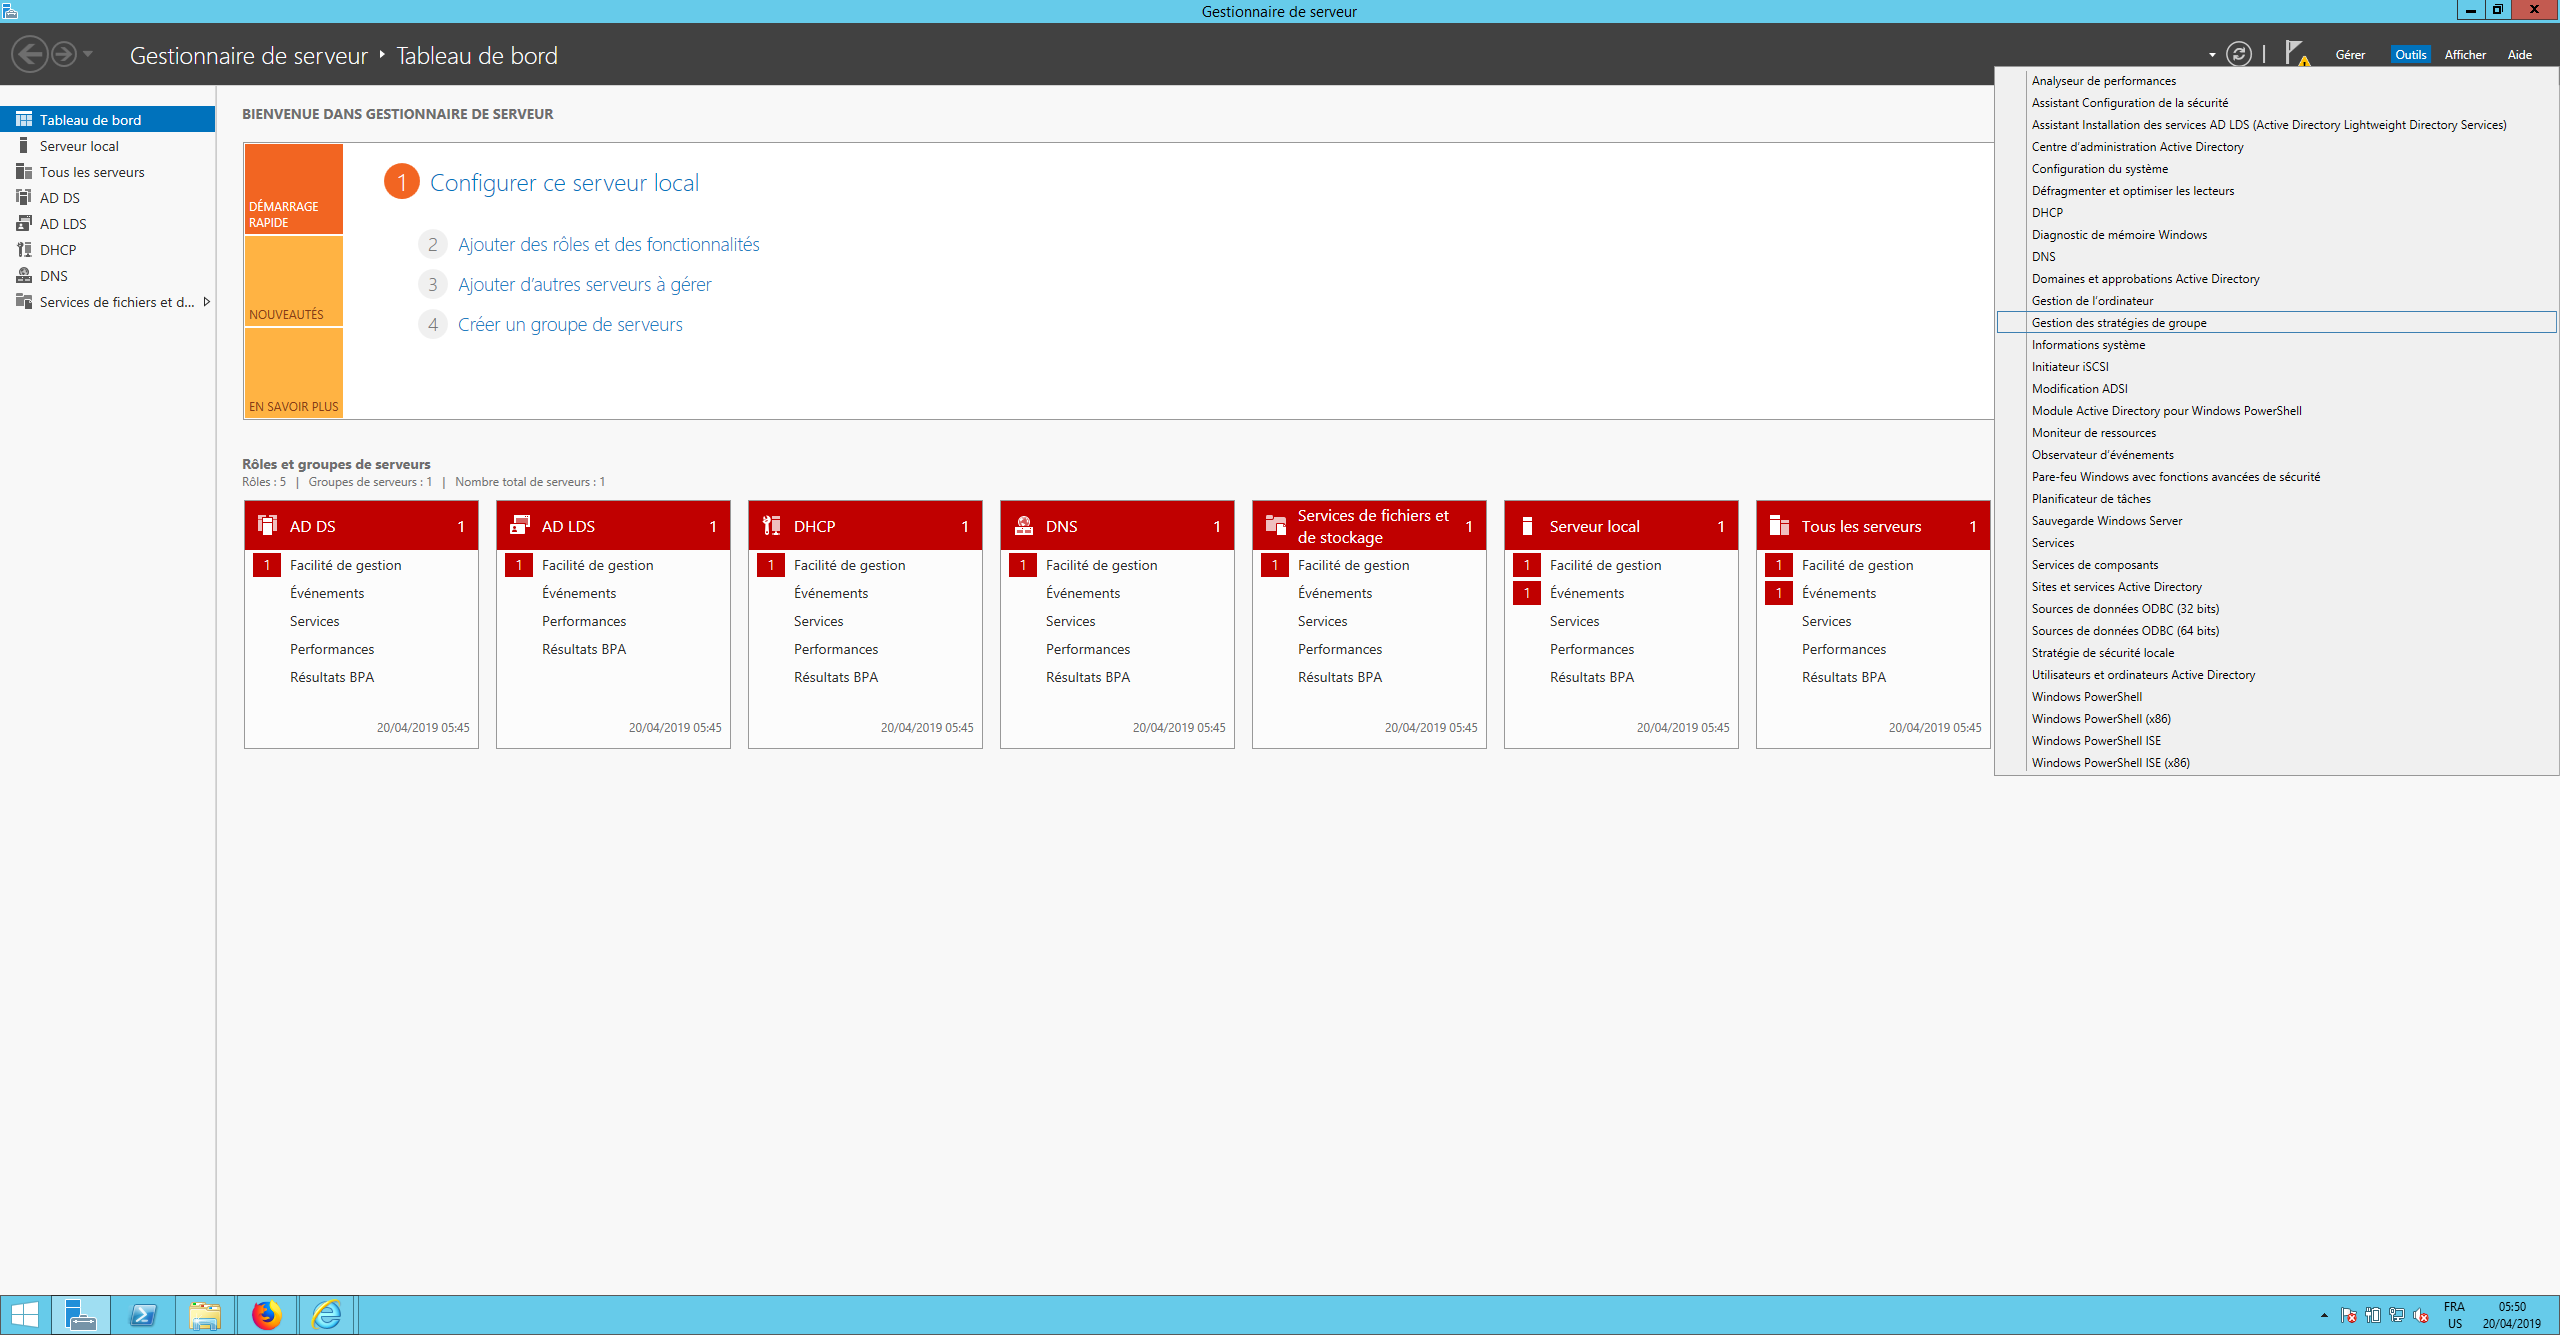
\includegraphics[scale=0.20]{Interception_Screenshots/GPO0.png}
        \caption{Accès aux politiques de groupe pour l'interception TLS}
    \end{center}
\end{figure}
\FloatBarrier


\item Dérouler le menu comme suit : \textbf{Gestion de stratégie de groupe -> Forêt : EPITAF.local -> Domaines -> EPITAF.local -> Objets de stratégie de groupe} puis cliquer sur \textbf{Nouveau} ;
\begin{figure}[h!]
    \begin{center}
        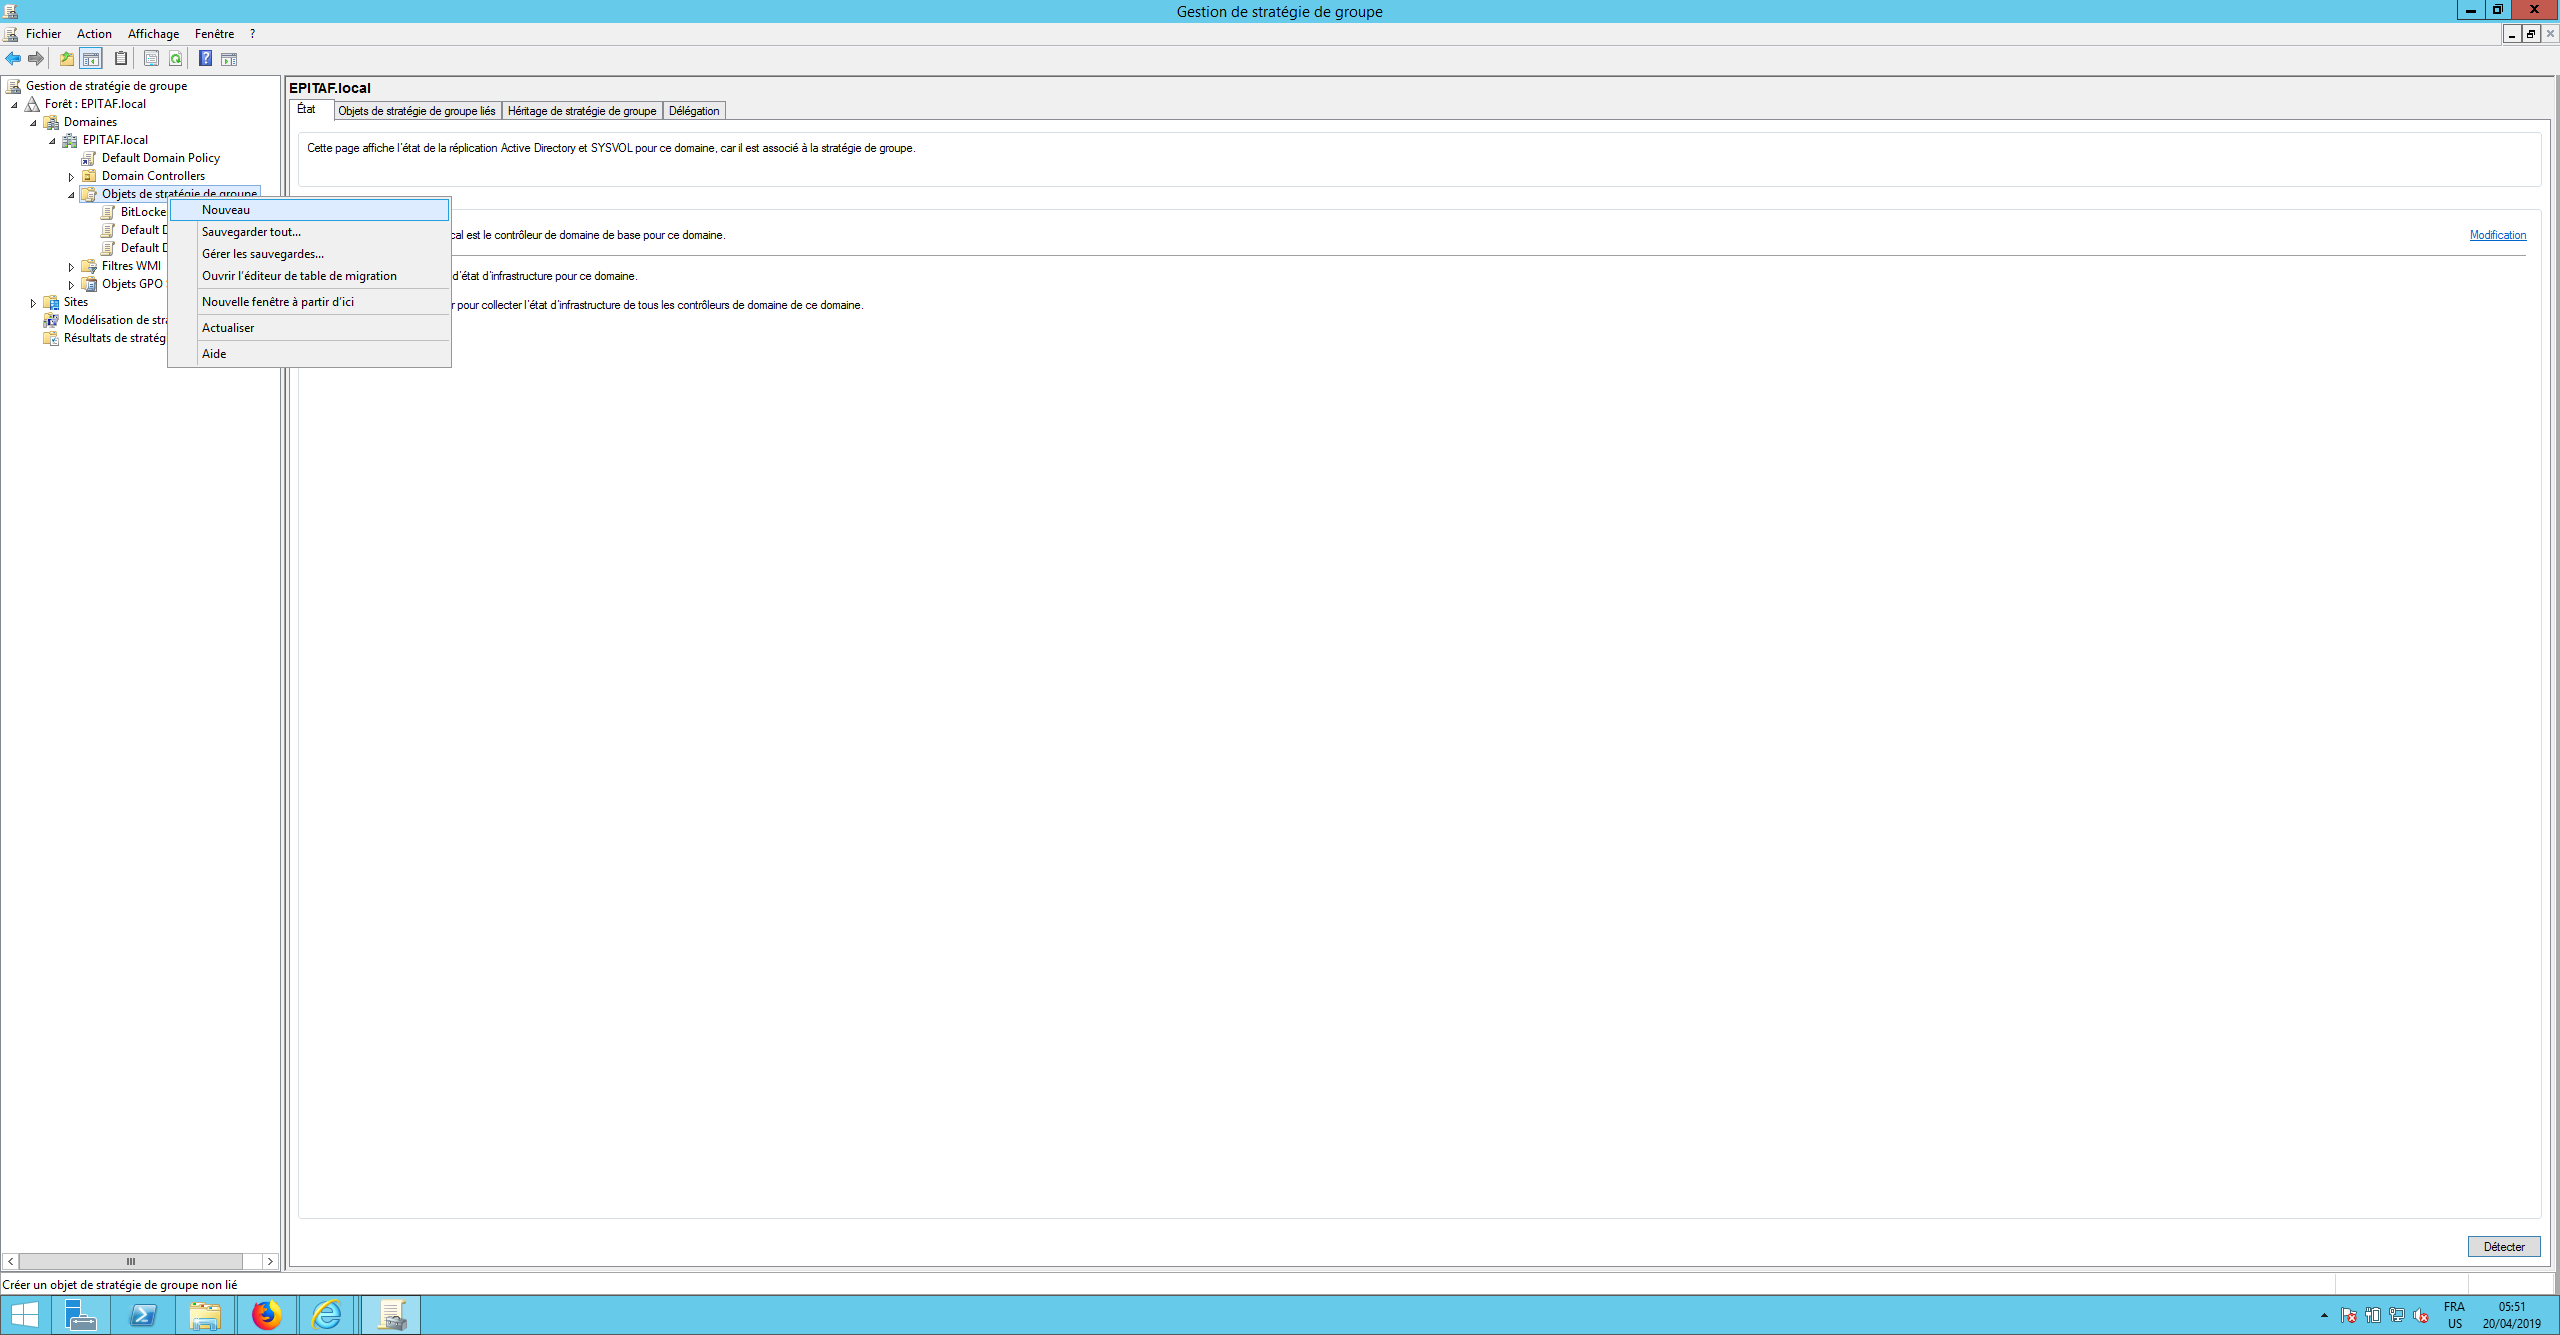
\includegraphics[scale=0.20]{Interception_Screenshots/GPO1.png}
        \caption{Nouvelle GPO pour l'interception TLS}
    \end{center}
\end{figure}
\FloatBarrier

\item Indiquer le nom de la GPO et cliquer sur \textit{OK} ;
\begin{figure}[h!]
    \begin{center}
        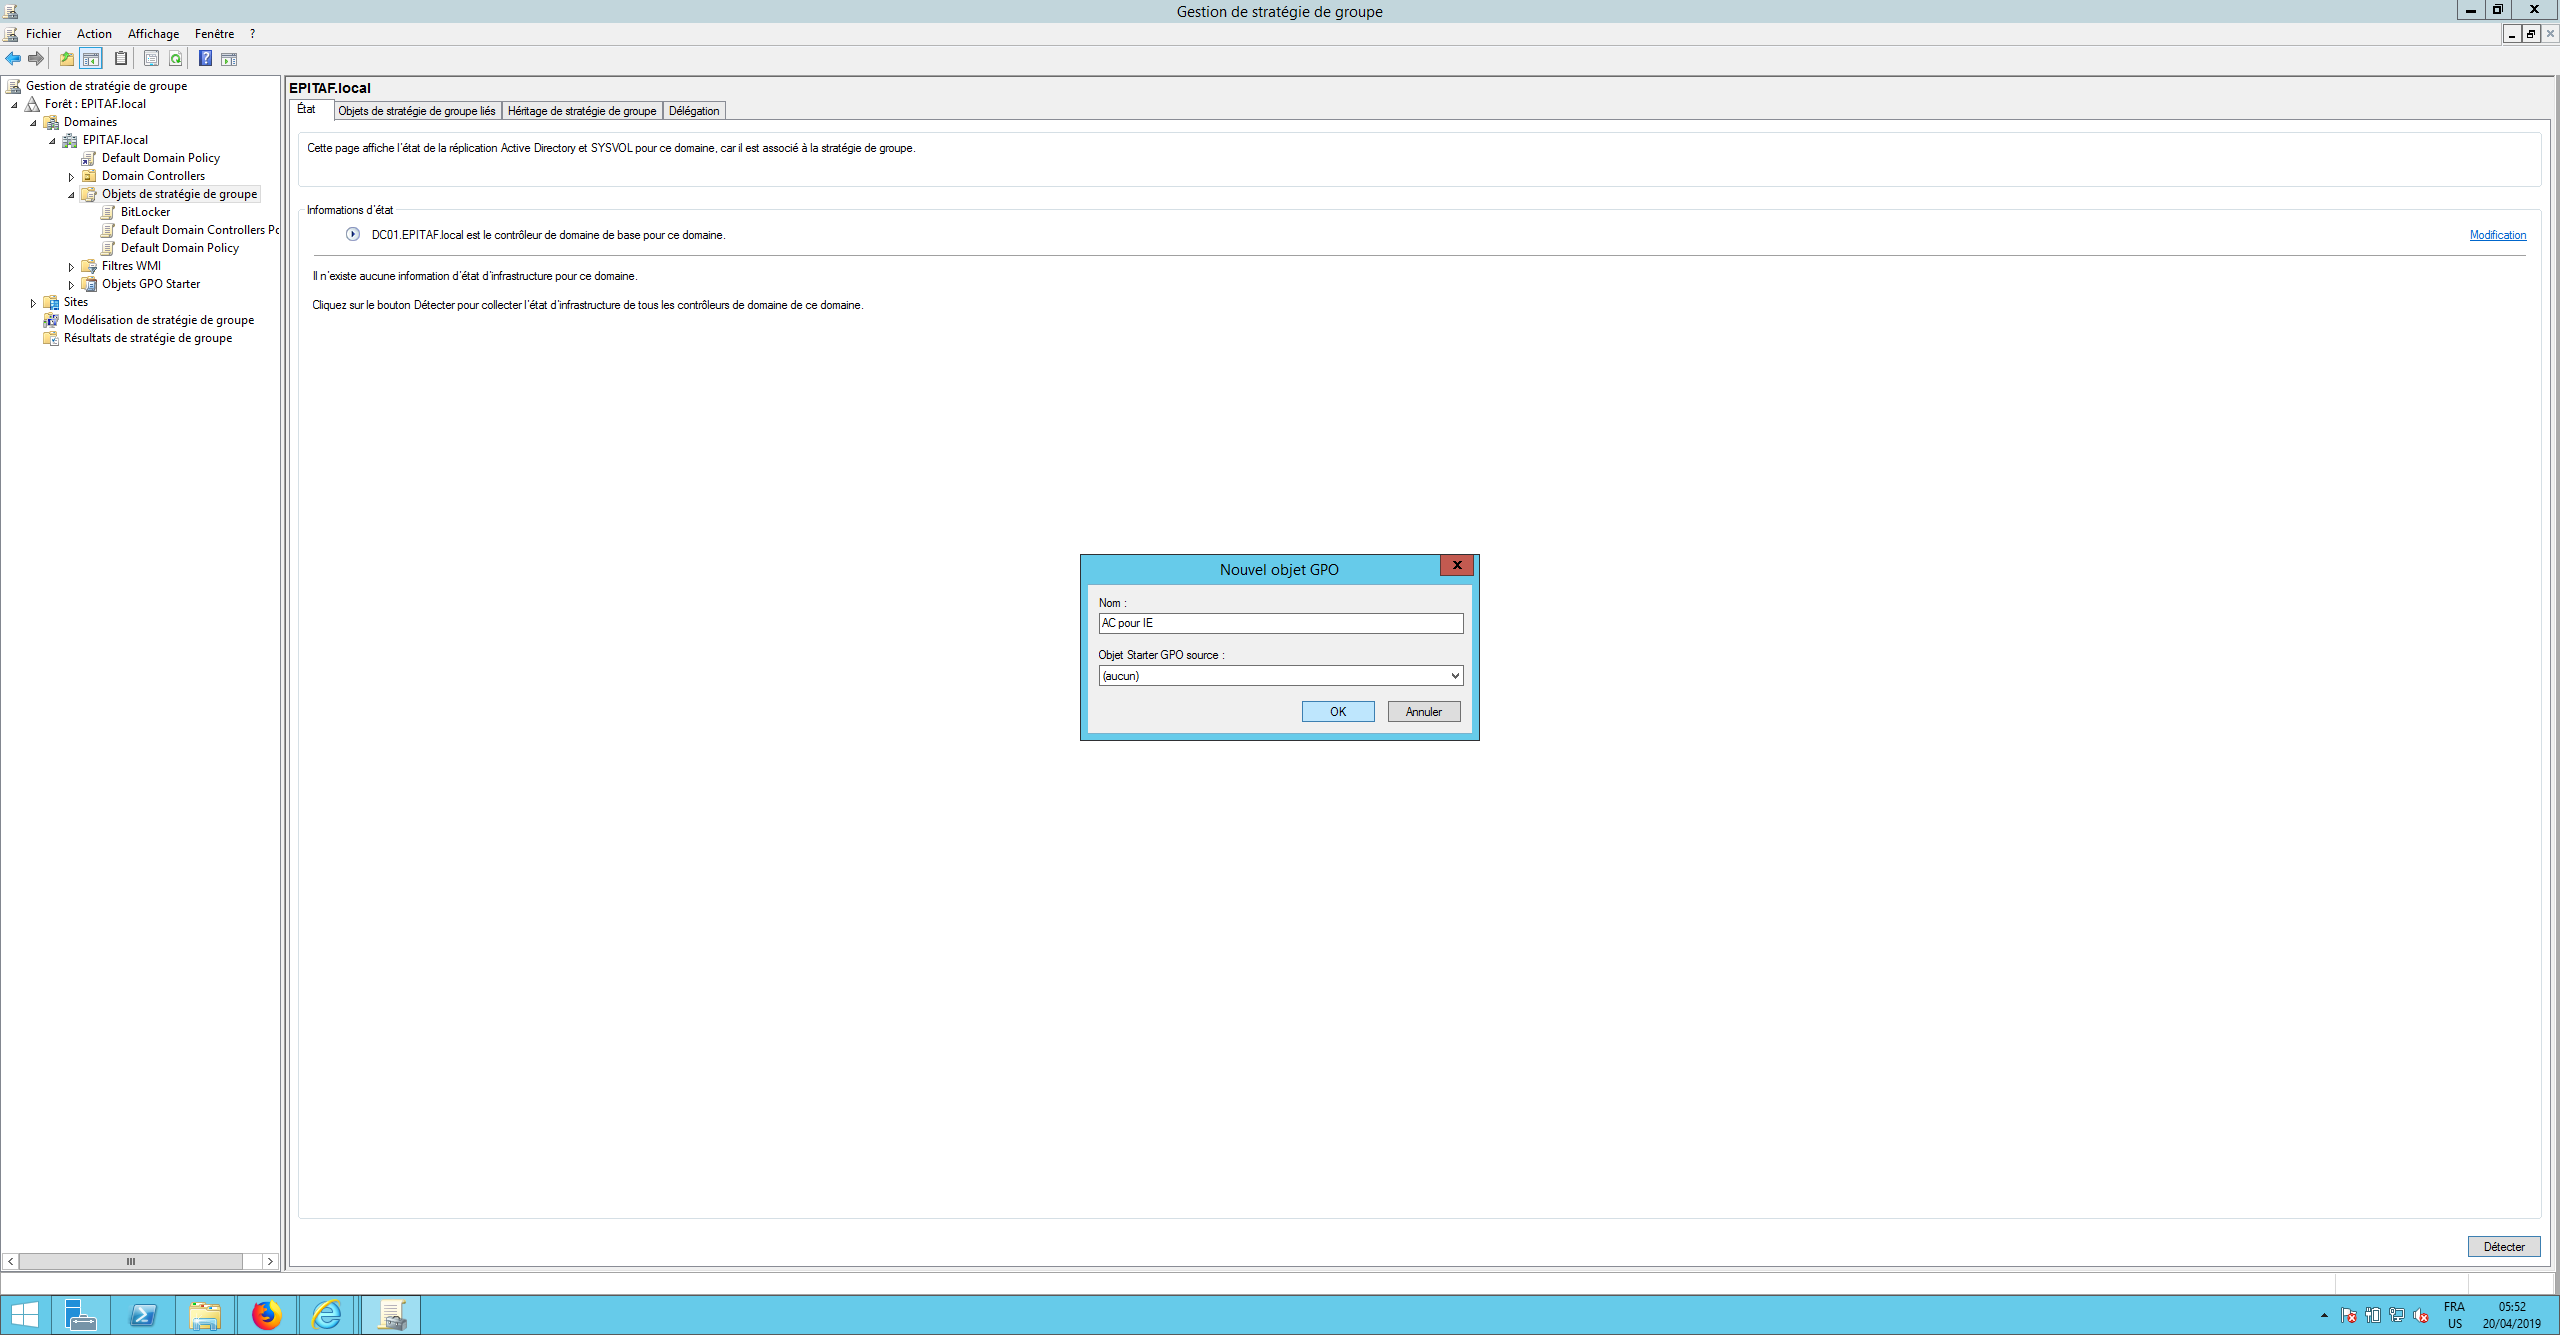
\includegraphics[scale=0.20]{Interception_Screenshots/GPO2.png}
        \caption{Nom de la nouvelle GPO pour l'interception TLS}
    \end{center}
\end{figure}
\FloatBarrier 

\item Cliquer droit sur la nouvelle GPO puis cliquer sur \textit{Modifier...} ;
\begin{figure}[h!]
    \begin{center}
        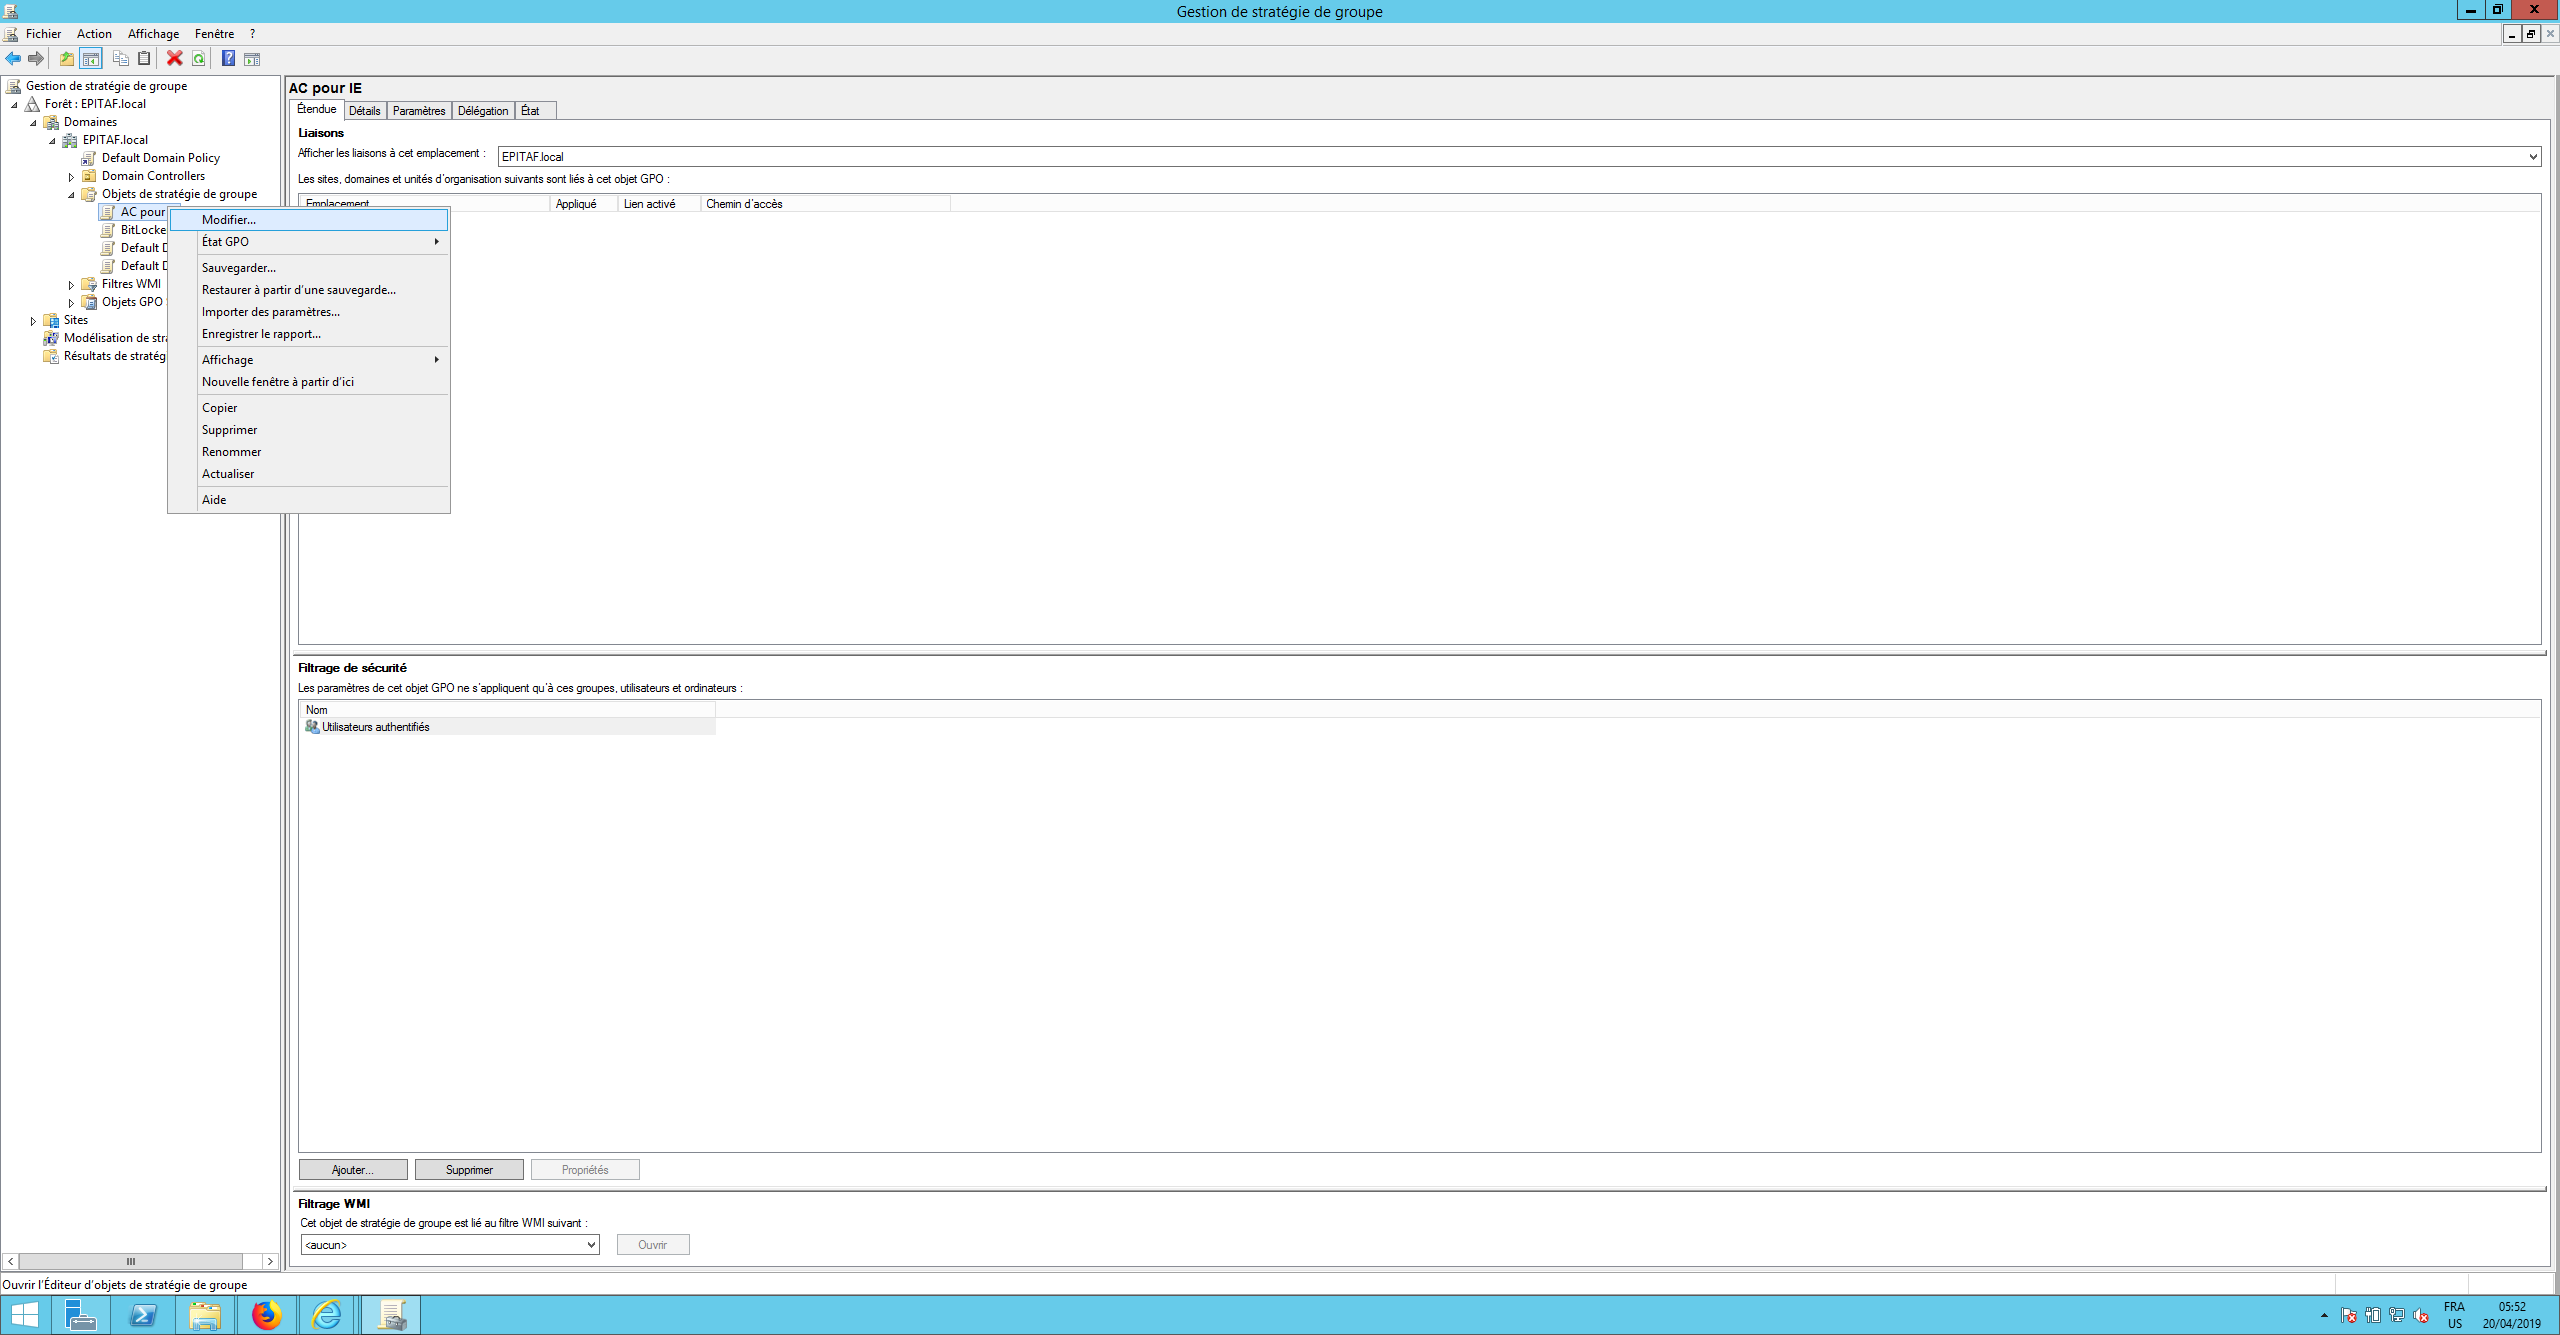
\includegraphics[scale=0.20]{Interception_Screenshots/GPO3.png}
        \caption{Modification de la GPO pour l'interception TLS}
    \end{center}
\end{figure}
\FloatBarrier 

\item Dérouler le menu comme suit : \textbf{Stratégie AC pour IE -> Configuration -> Paramètres Windows -> Paramètres de sécurité -> Stratégie de clé publique} puis cliquer droit sur \textbf{Autorité de certification racines de confiance} ;
\item Cliquer sur \textbf{Importer...} ;
\begin{figure}[h!]
    \begin{center}
        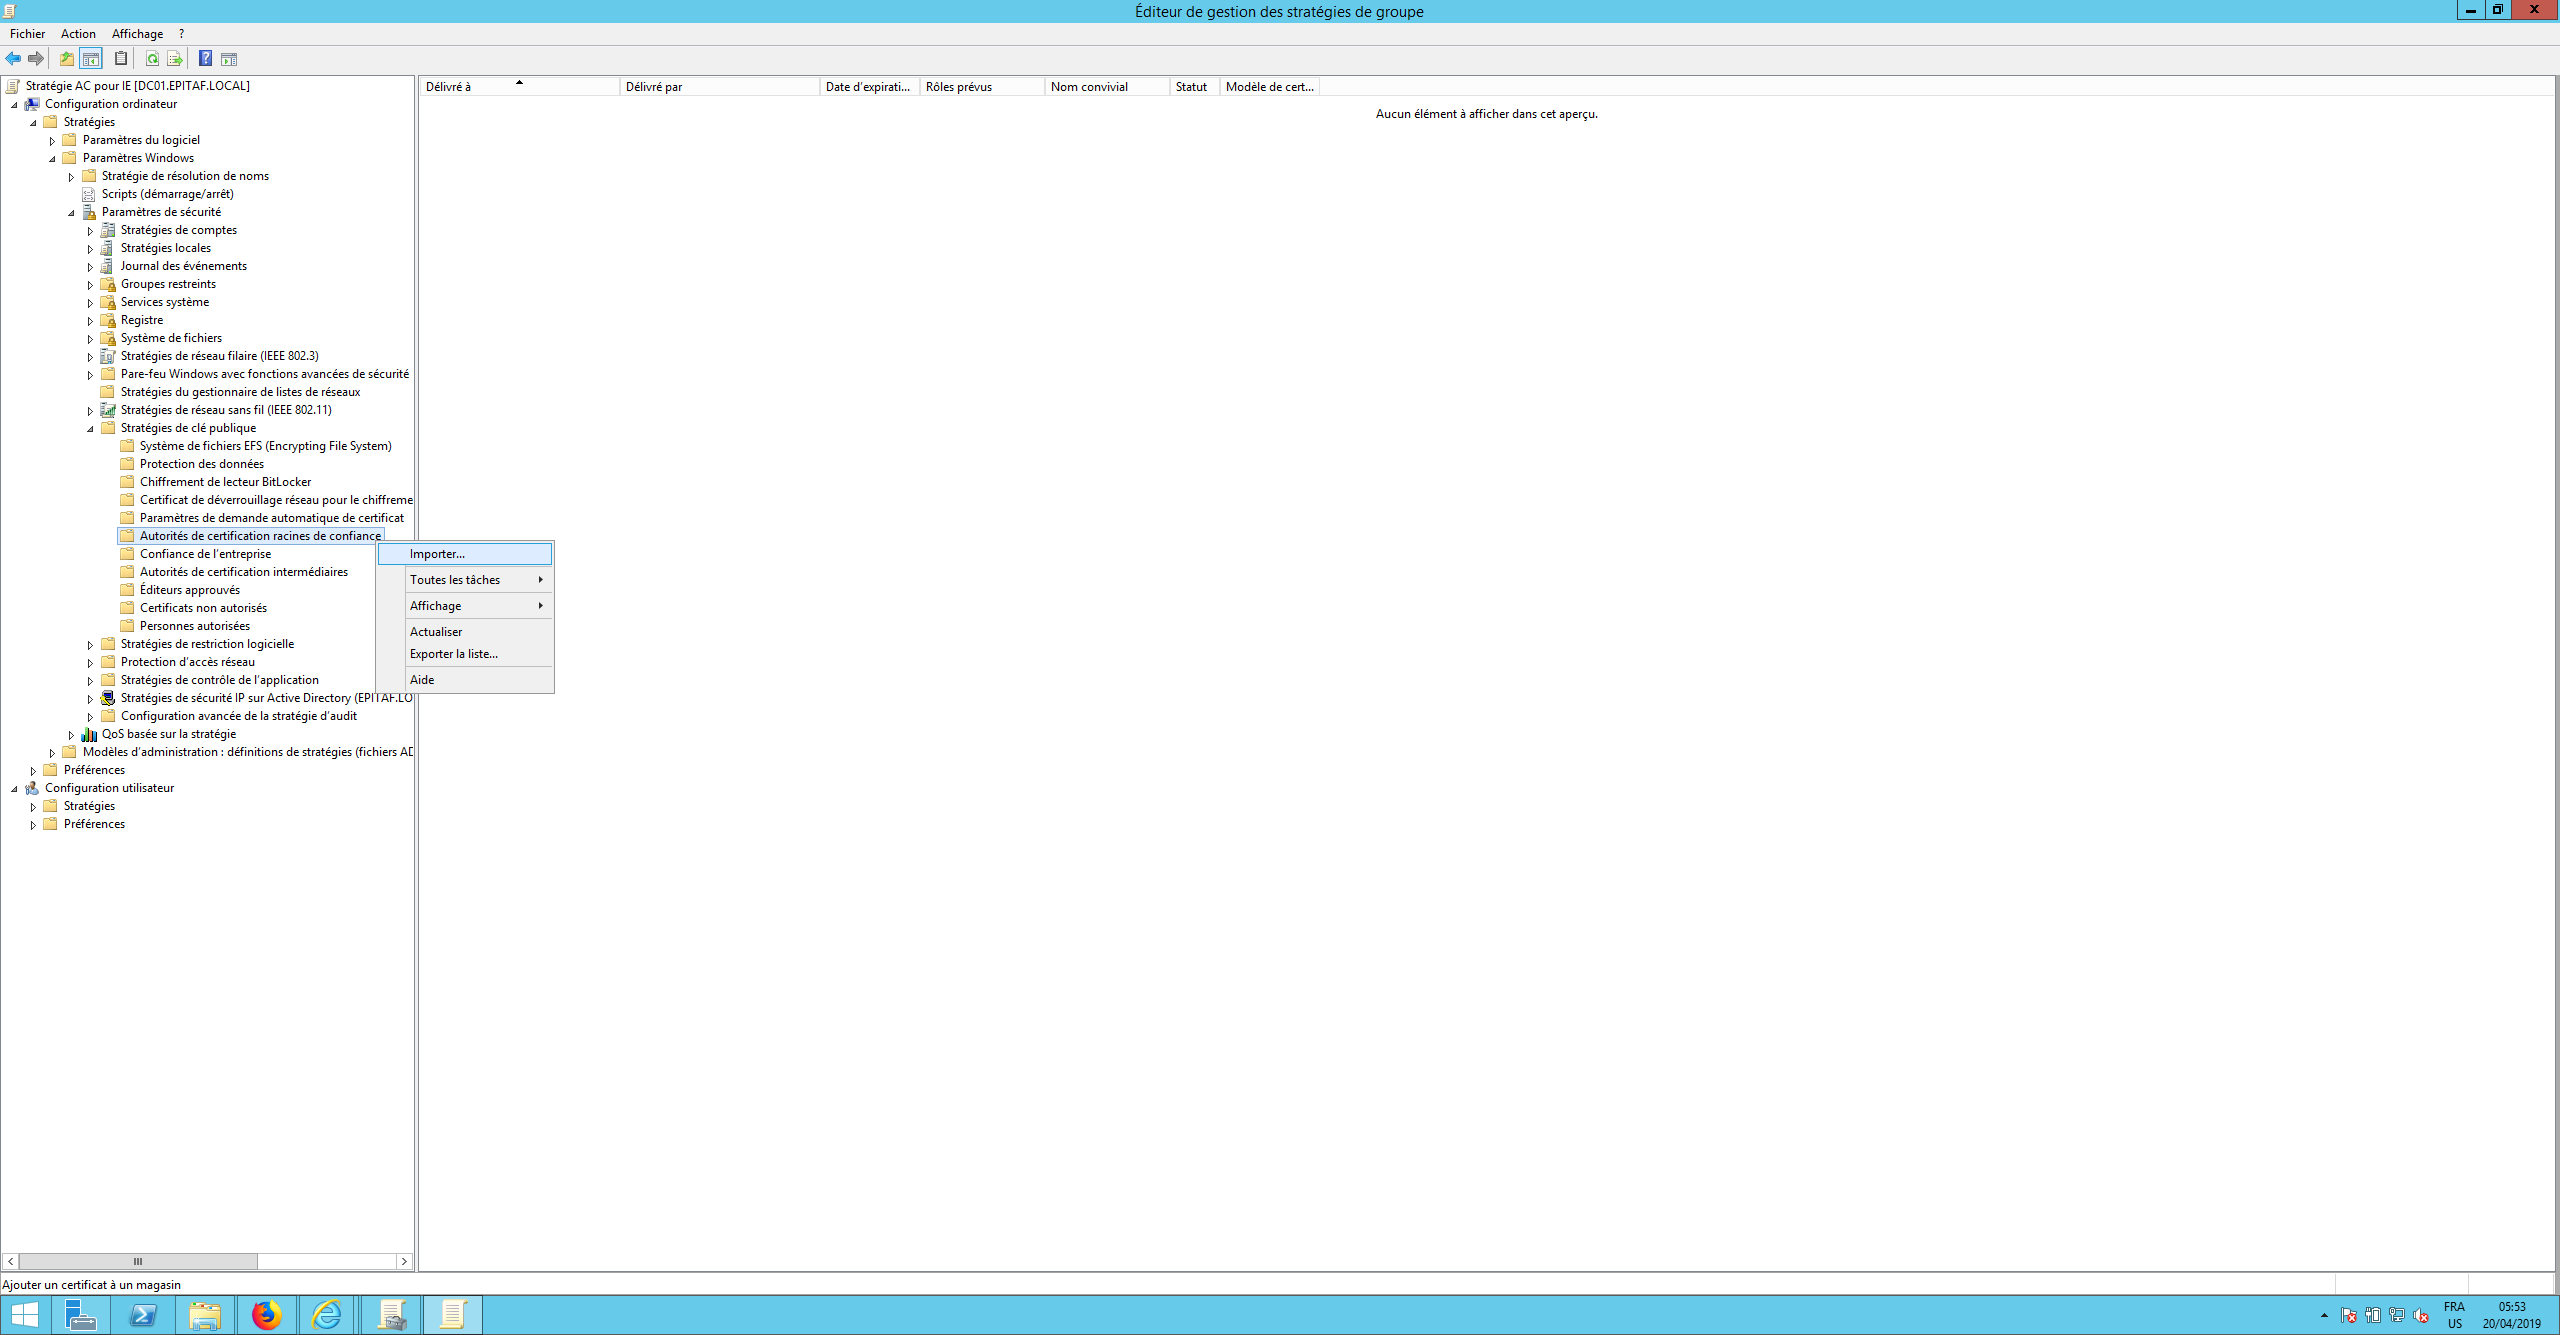
\includegraphics[scale=0.20]{Interception_Screenshots/GPO4.png}
        \caption{Ajout du certificat pour la nouvelle GPO pour l'interception TLS}
    \end{center}
\end{figure}
\FloatBarrier 

\item Cliquer sur \textit{Suivant} ;
\begin{figure}[h!]
    \begin{center}
        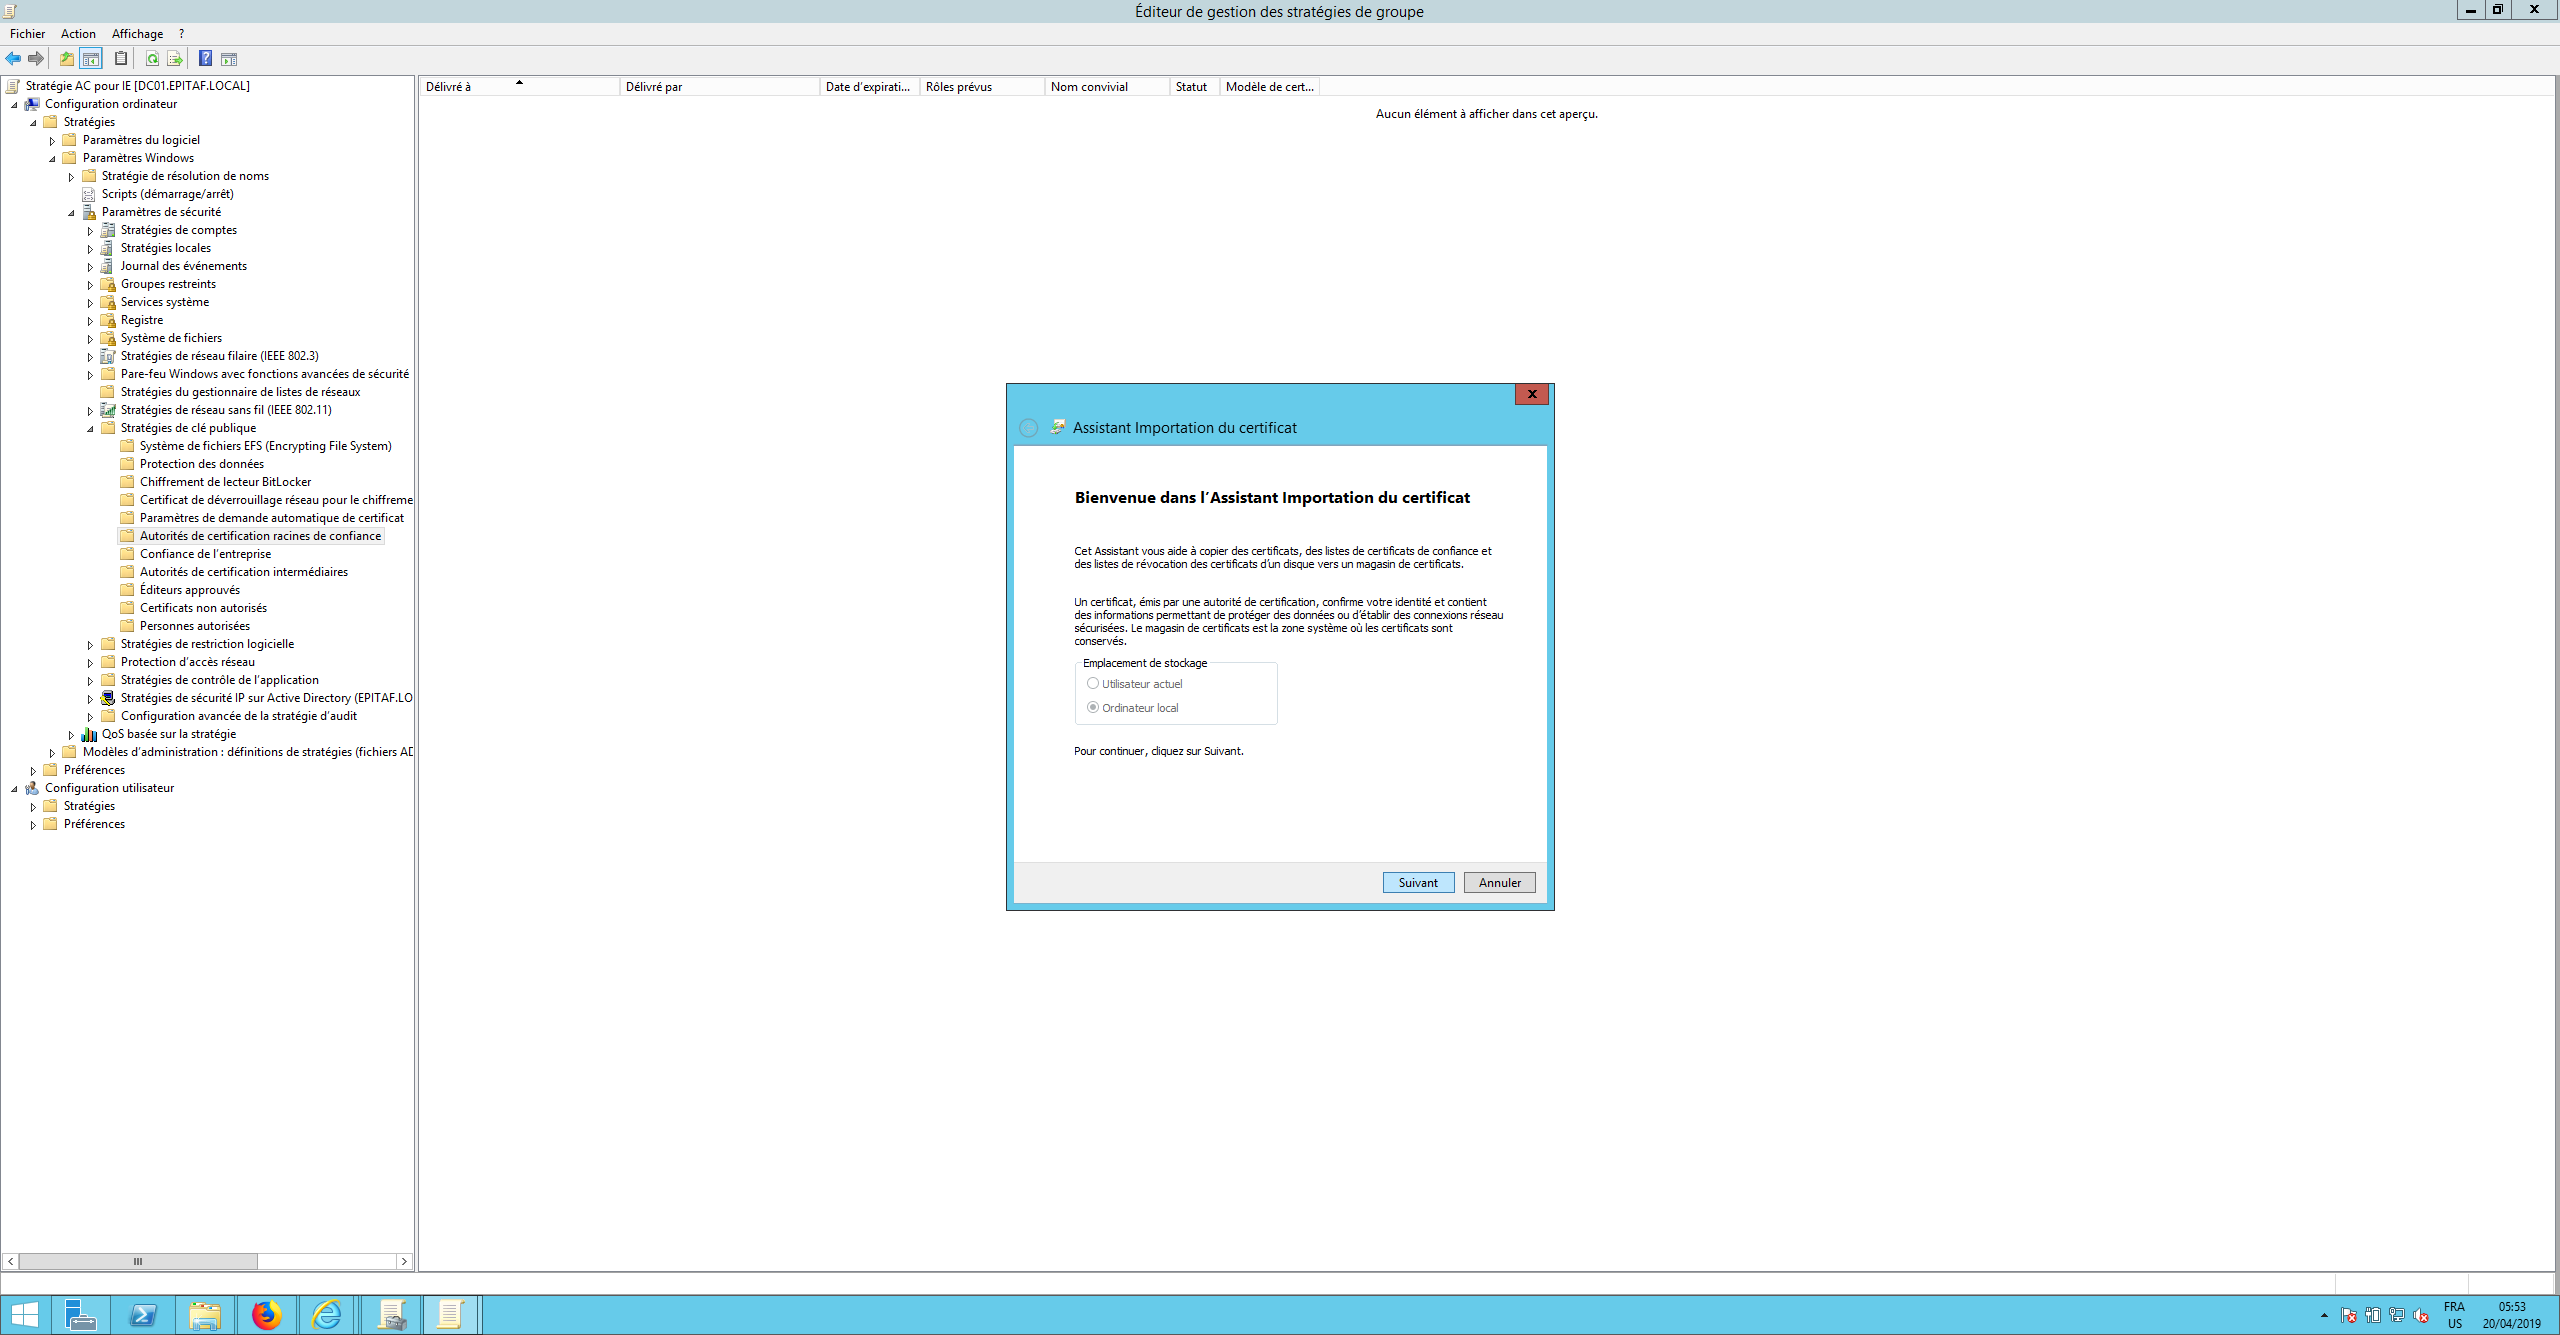
\includegraphics[scale=0.20]{Interception_Screenshots/GPO5.png}
        \caption{Nouveau CA pour l'interception TLS}
    \end{center}
\end{figure}
\FloatBarrier 

\item Cliquer sur \textbf{Parcourir...} ;
\item choisir le certificat puis cliquer sur \textit{Suivant} ;
\begin{figure}[h!]
    \begin{center}
        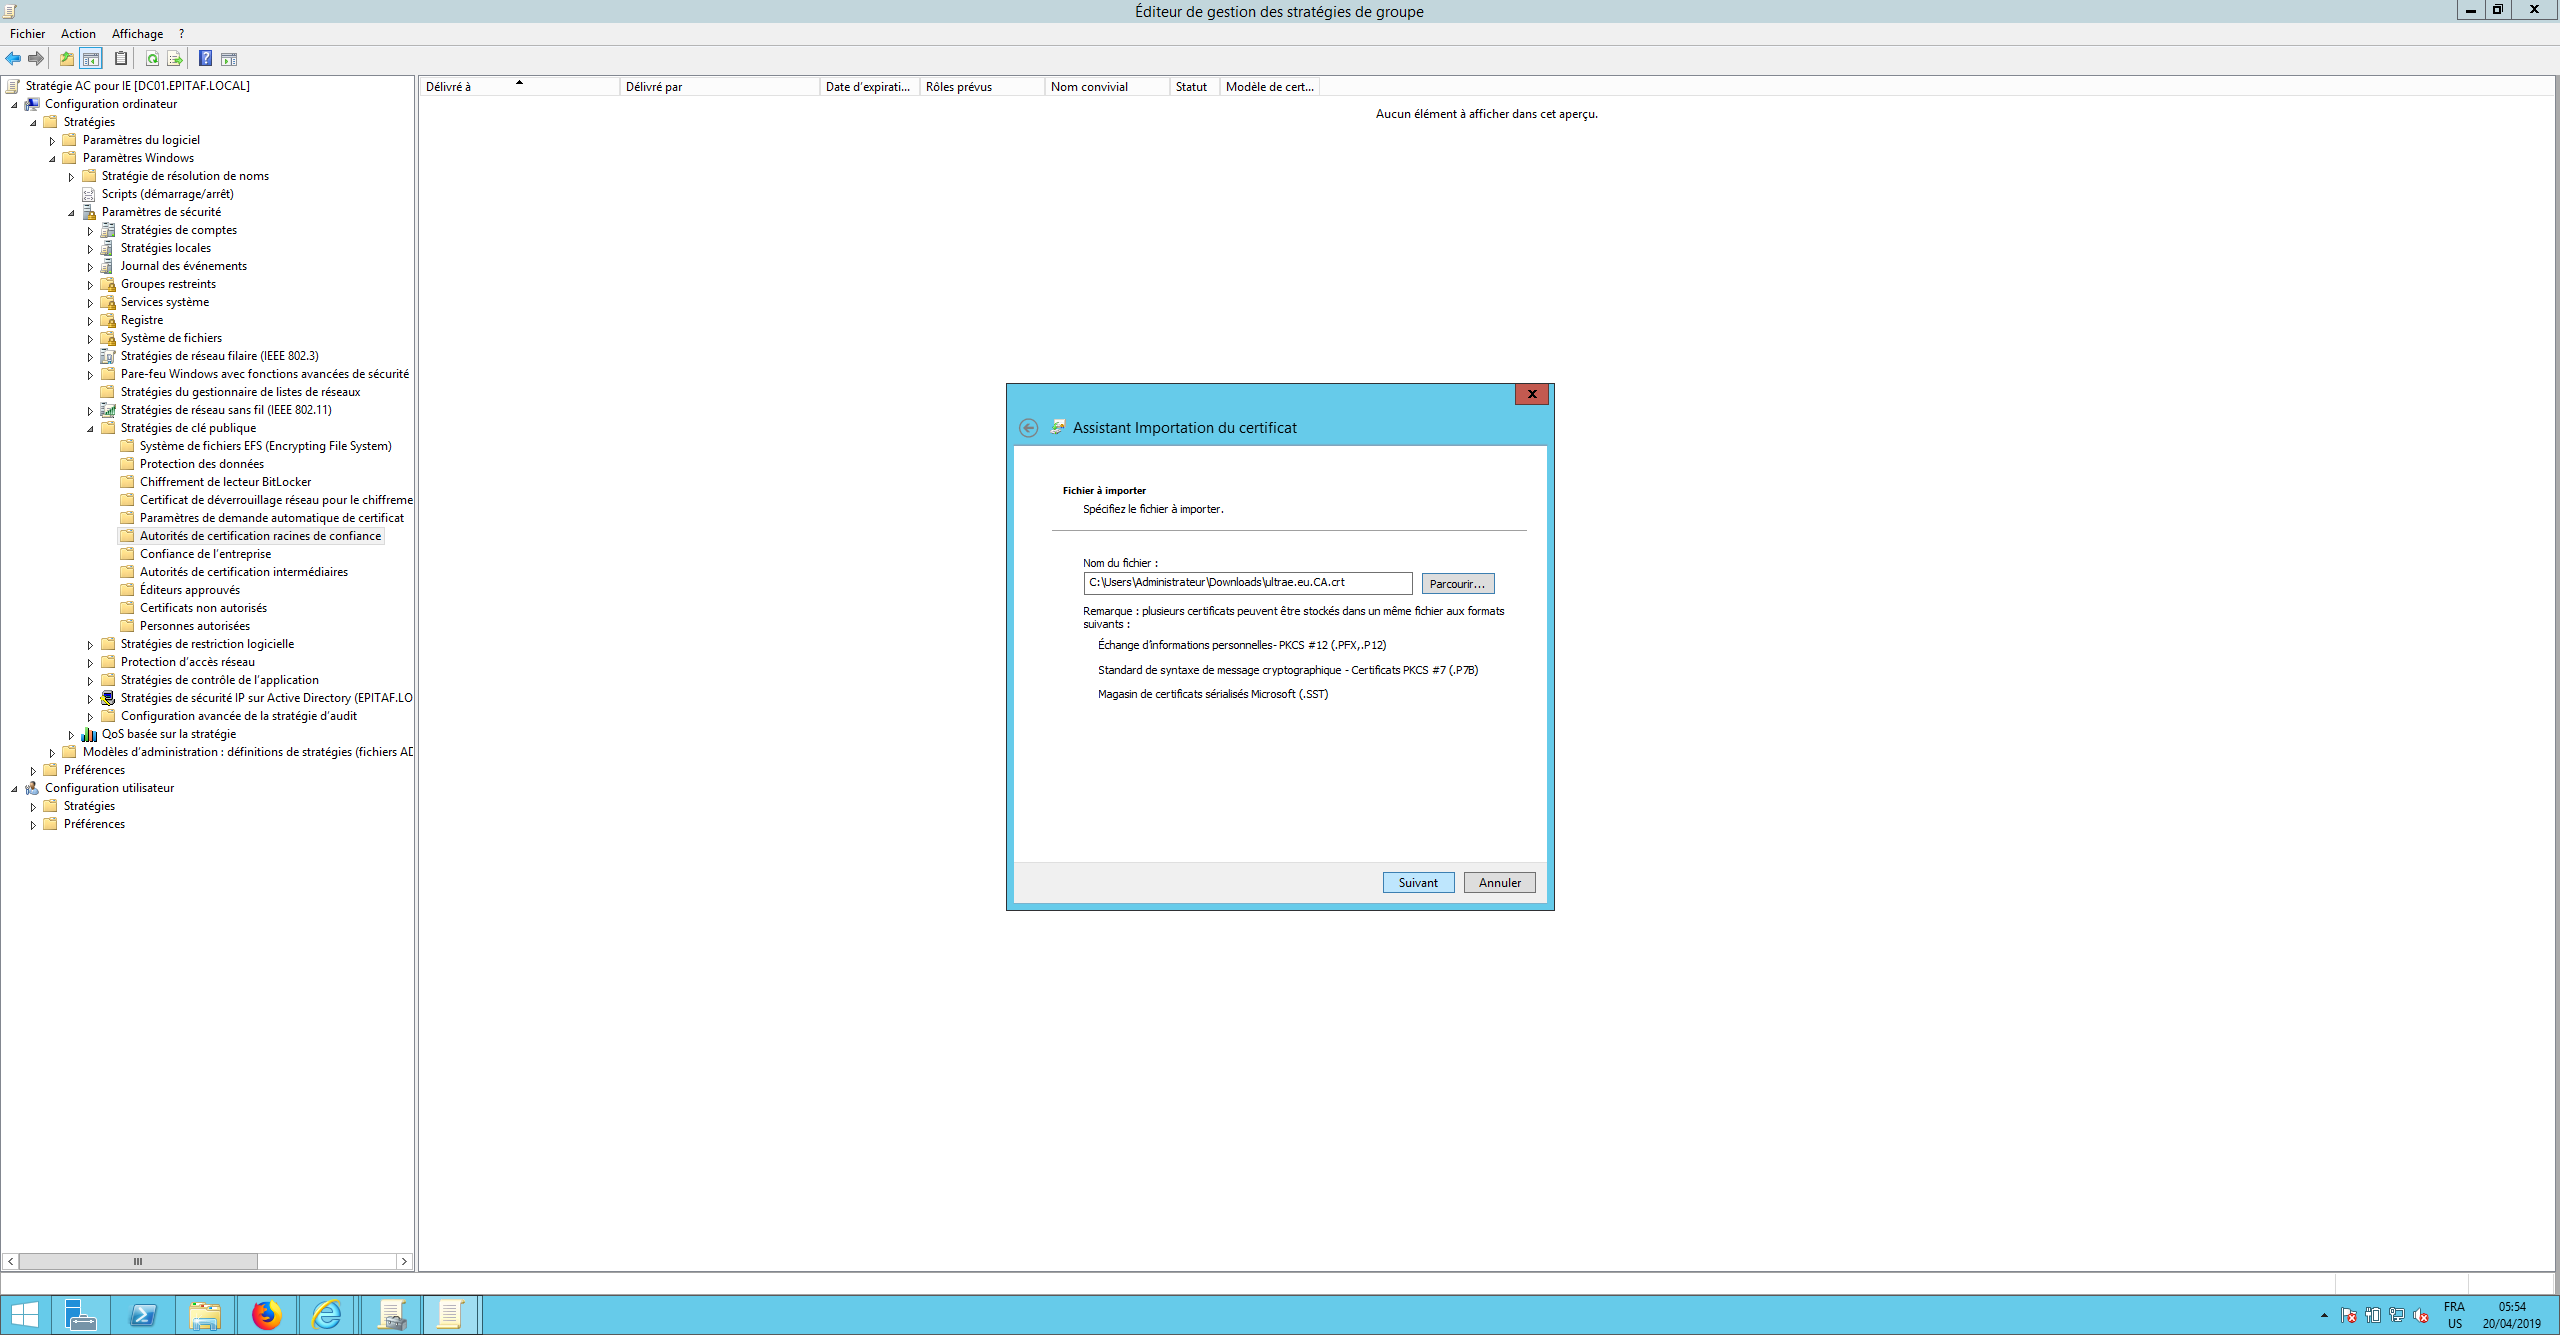
\includegraphics[scale=0.20]{Interception_Screenshots/GPO6.png}
        \caption{Choix du certificat pour la nouvelle GPO pour l'interception TLS}
    \end{center}
\end{figure}
\FloatBarrier 

\item Cliquer sur \textit{Suivant} ;
\begin{figure}[h!]
    \begin{center}
        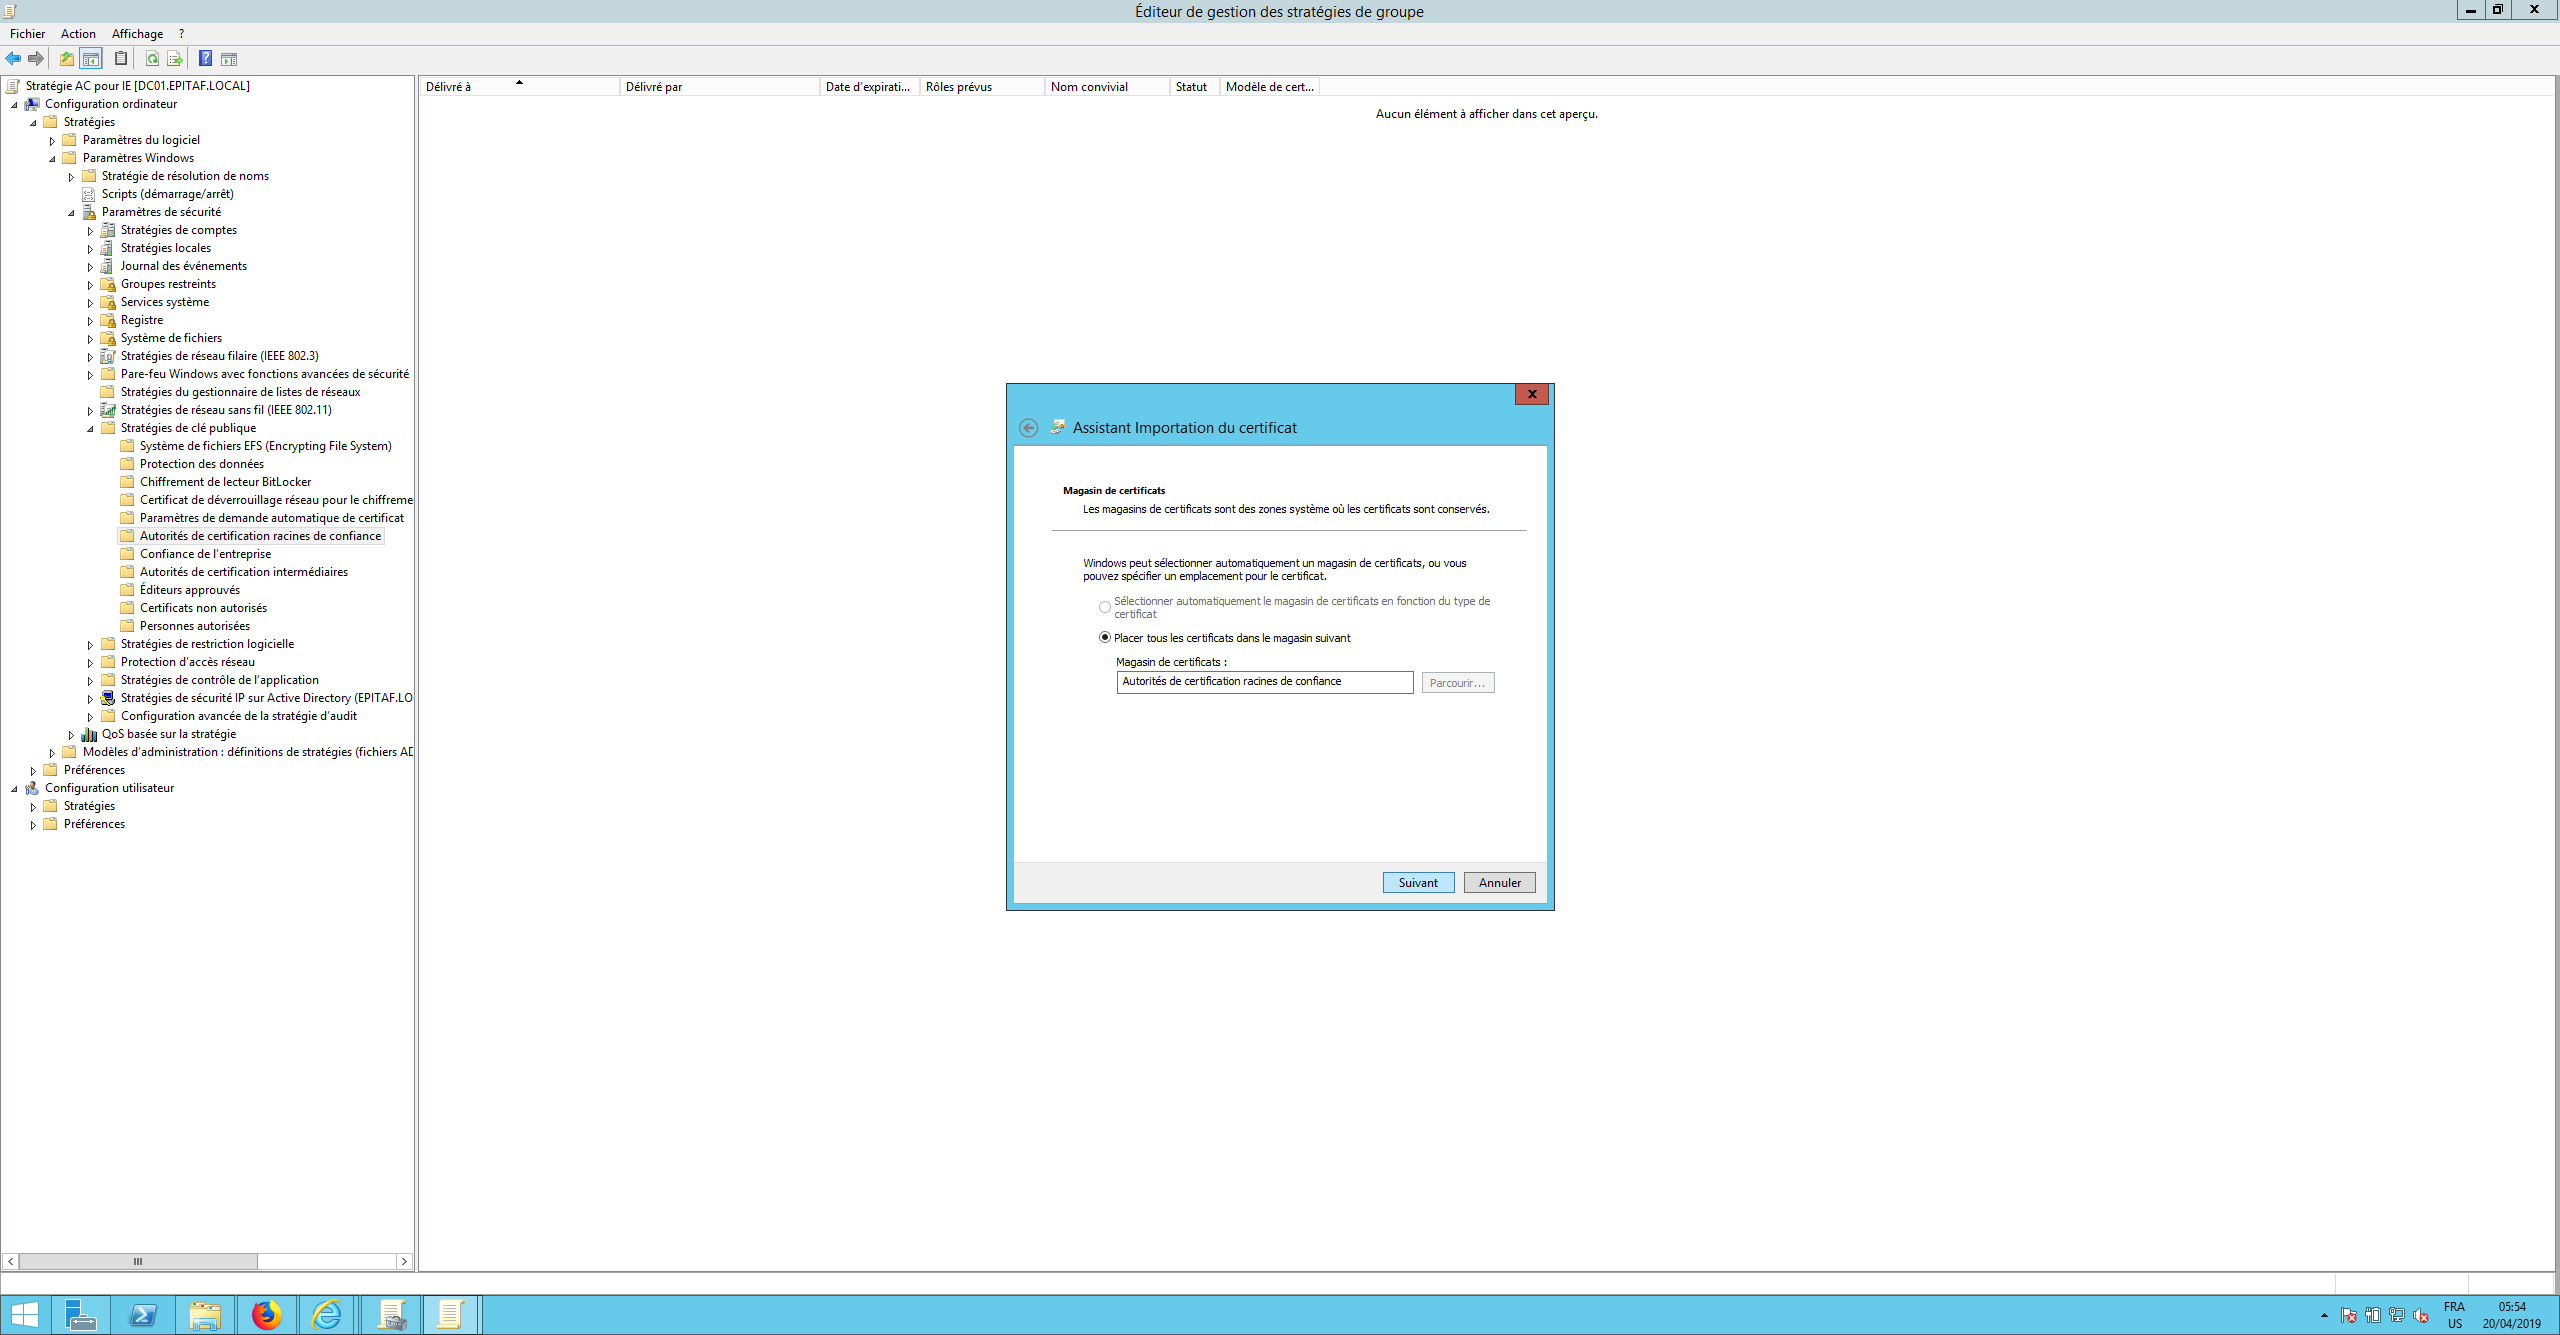
\includegraphics[scale=0.20]{Interception_Screenshots/GPO7.png}
        \caption{Placement du CA pour l'interception TLS}
    \end{center}
\end{figure}
\FloatBarrier 

\item Cliquer sur \textit{Terminer} ;
\begin{figure}[h!]
    \begin{center}
        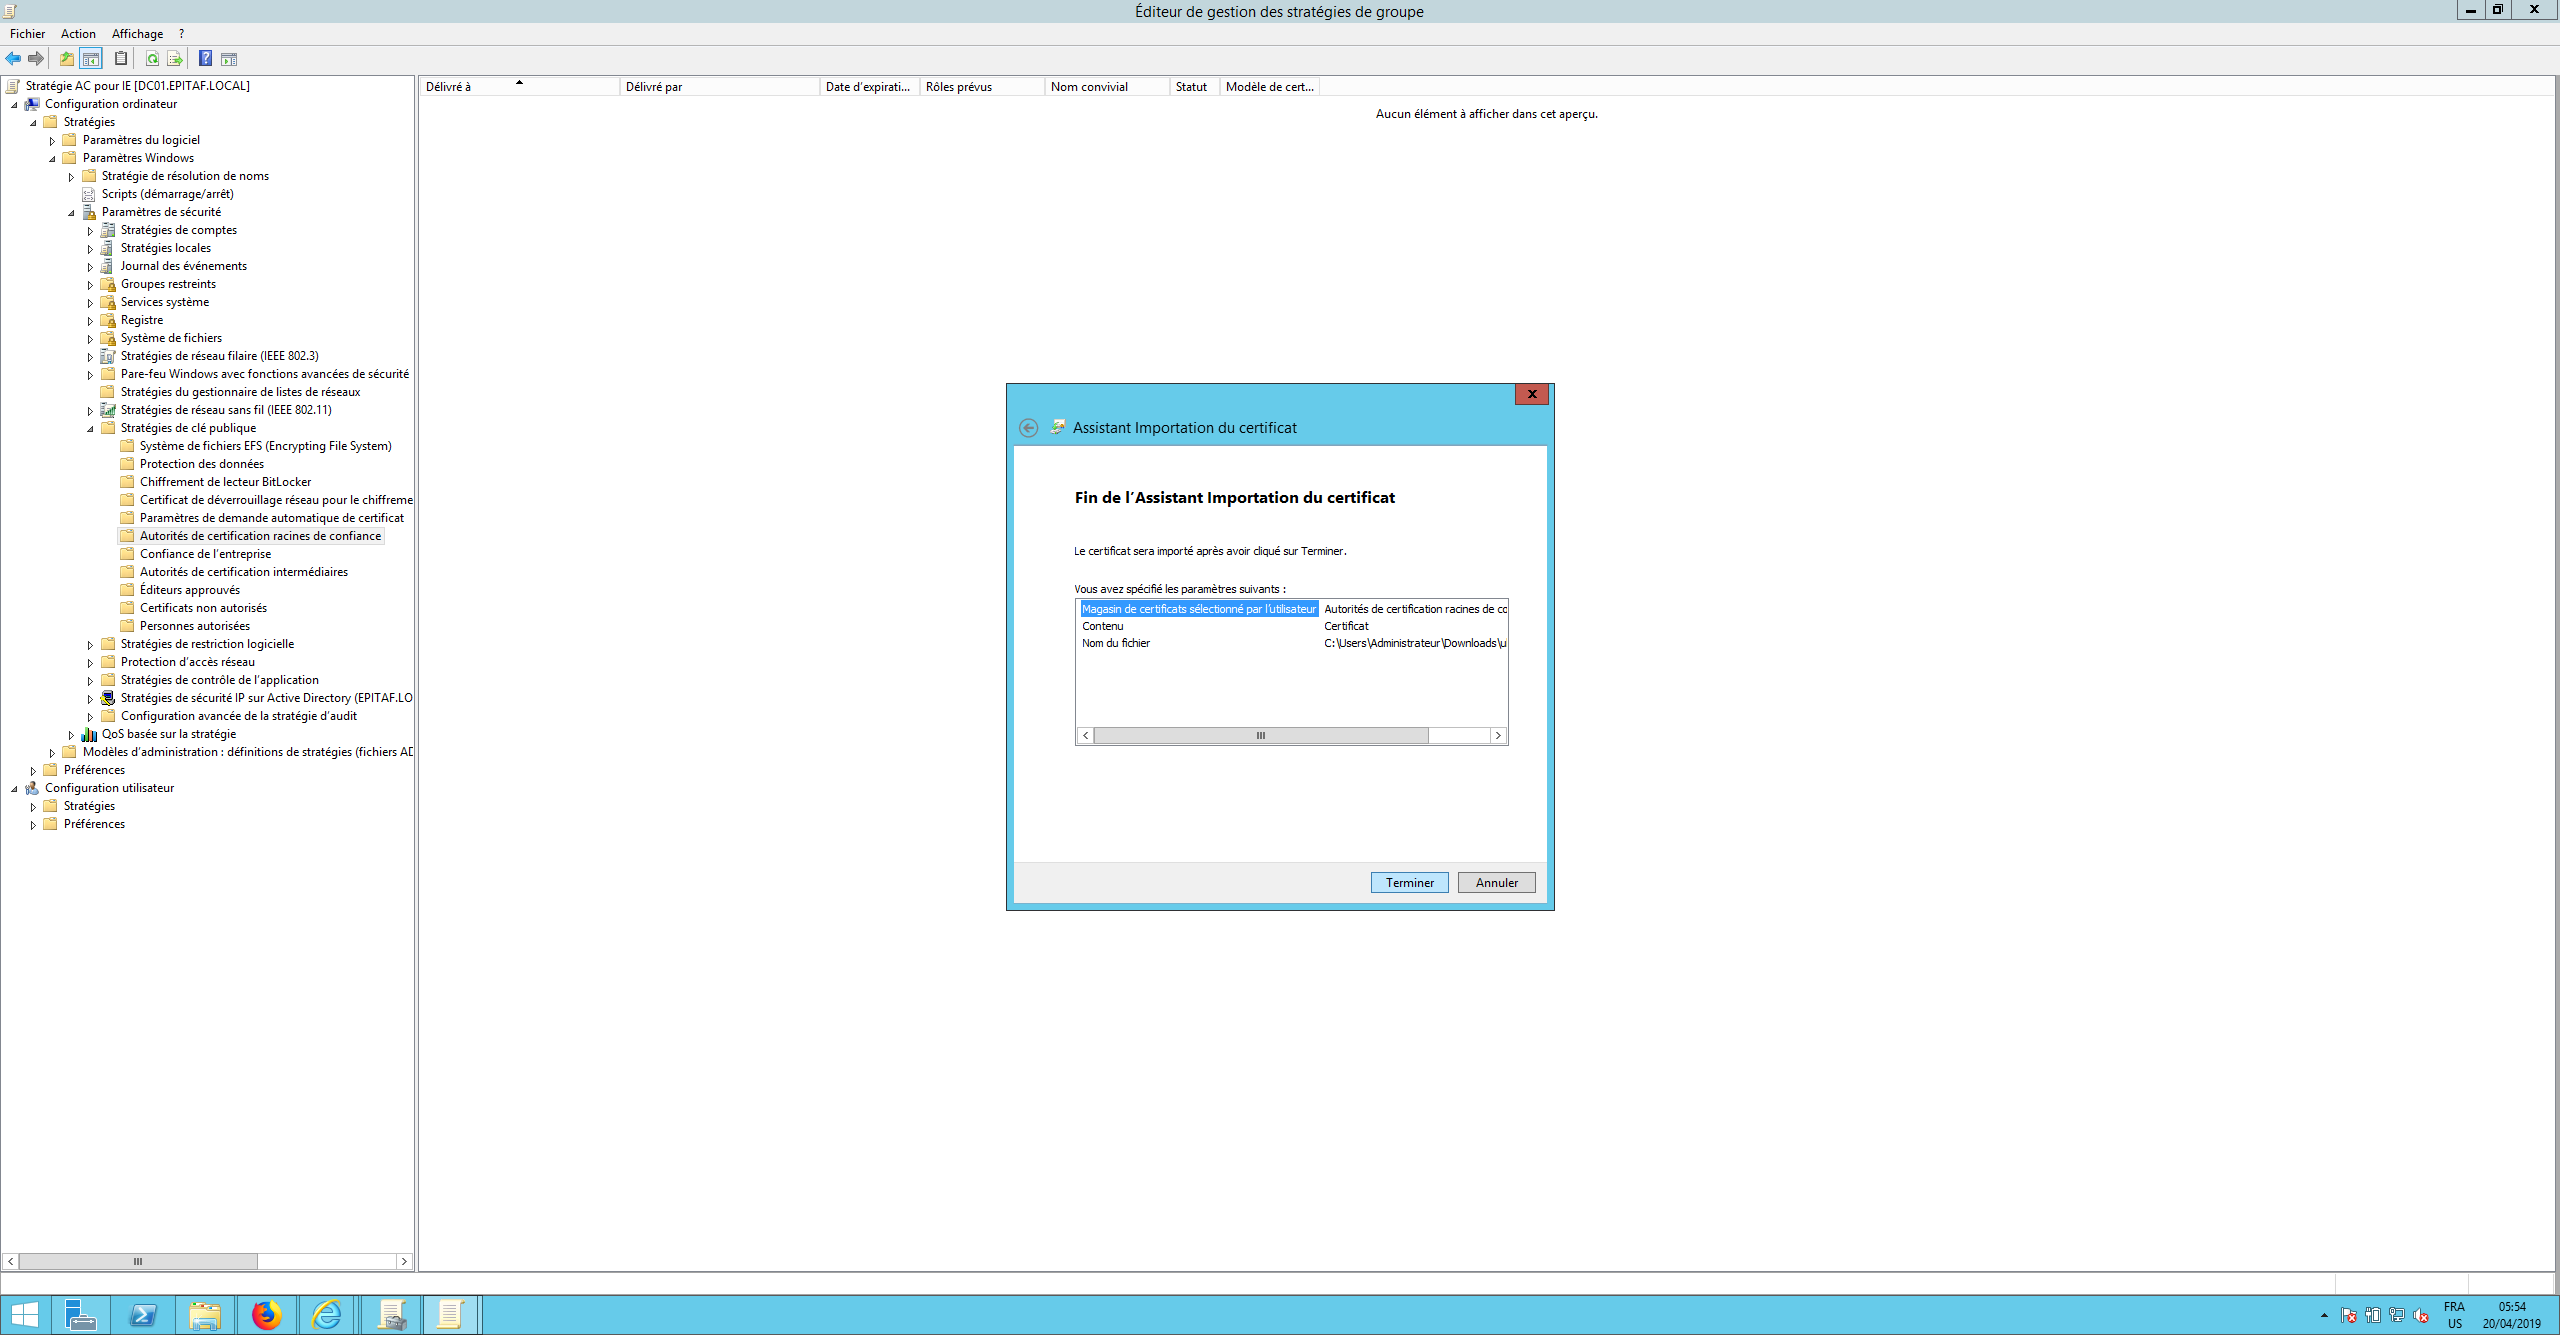
\includegraphics[scale=0.20]{Interception_Screenshots/GPO8.png}
        \caption{Fin de l'installation du nouveau certificat pour l'interception TLS}
    \end{center}
\end{figure}
\FloatBarrier 

\item Cliquer sur \textit{Ok}.
\begin{figure}[h!]
    \begin{center}
        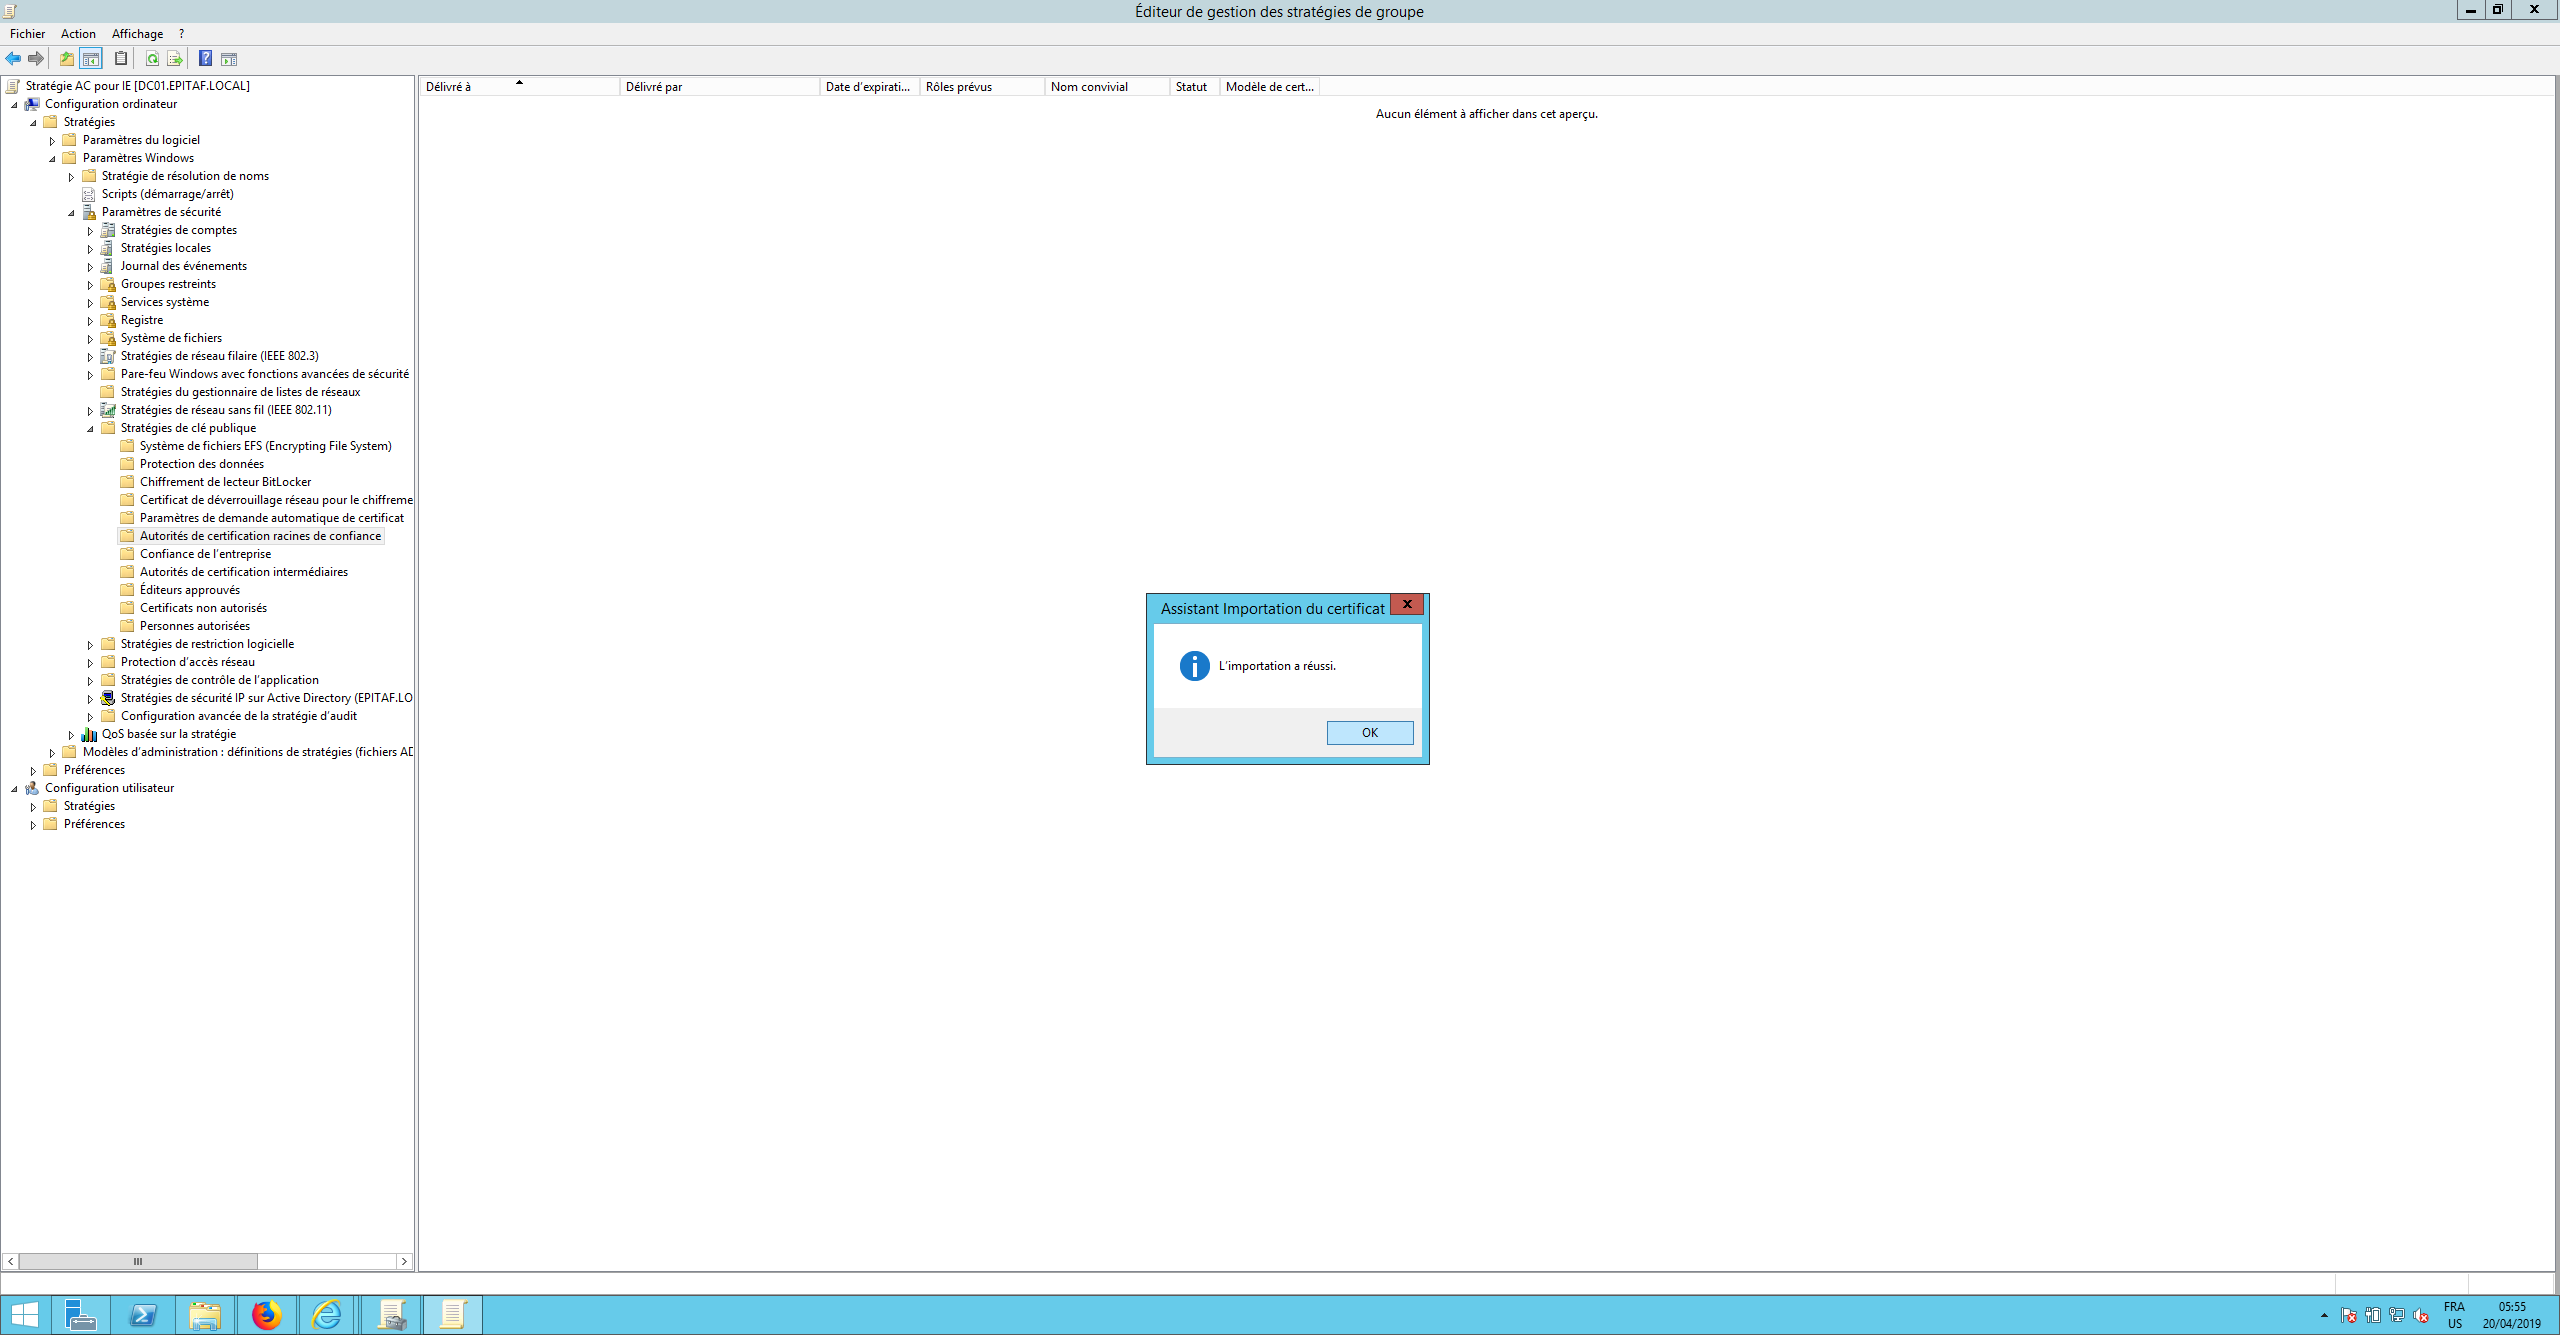
\includegraphics[scale=0.20]{Interception_Screenshots/GPO9.png}
        \caption{Validation de l'ajout du nouveau certificat pour l'interception TLS}
    \end{center}
\end{figure}
\FloatBarrier 

\end{itemize}


\subsection{Mise en place de l'antivirus ClamAV}

Pour mettre en place l'antivirus ClamAV, il faut :
\begin{itemize}
\item Accéder à \textbf{Services -> Squid Proxy Server} ;
\begin{figure}[h!]
    \begin{center}
        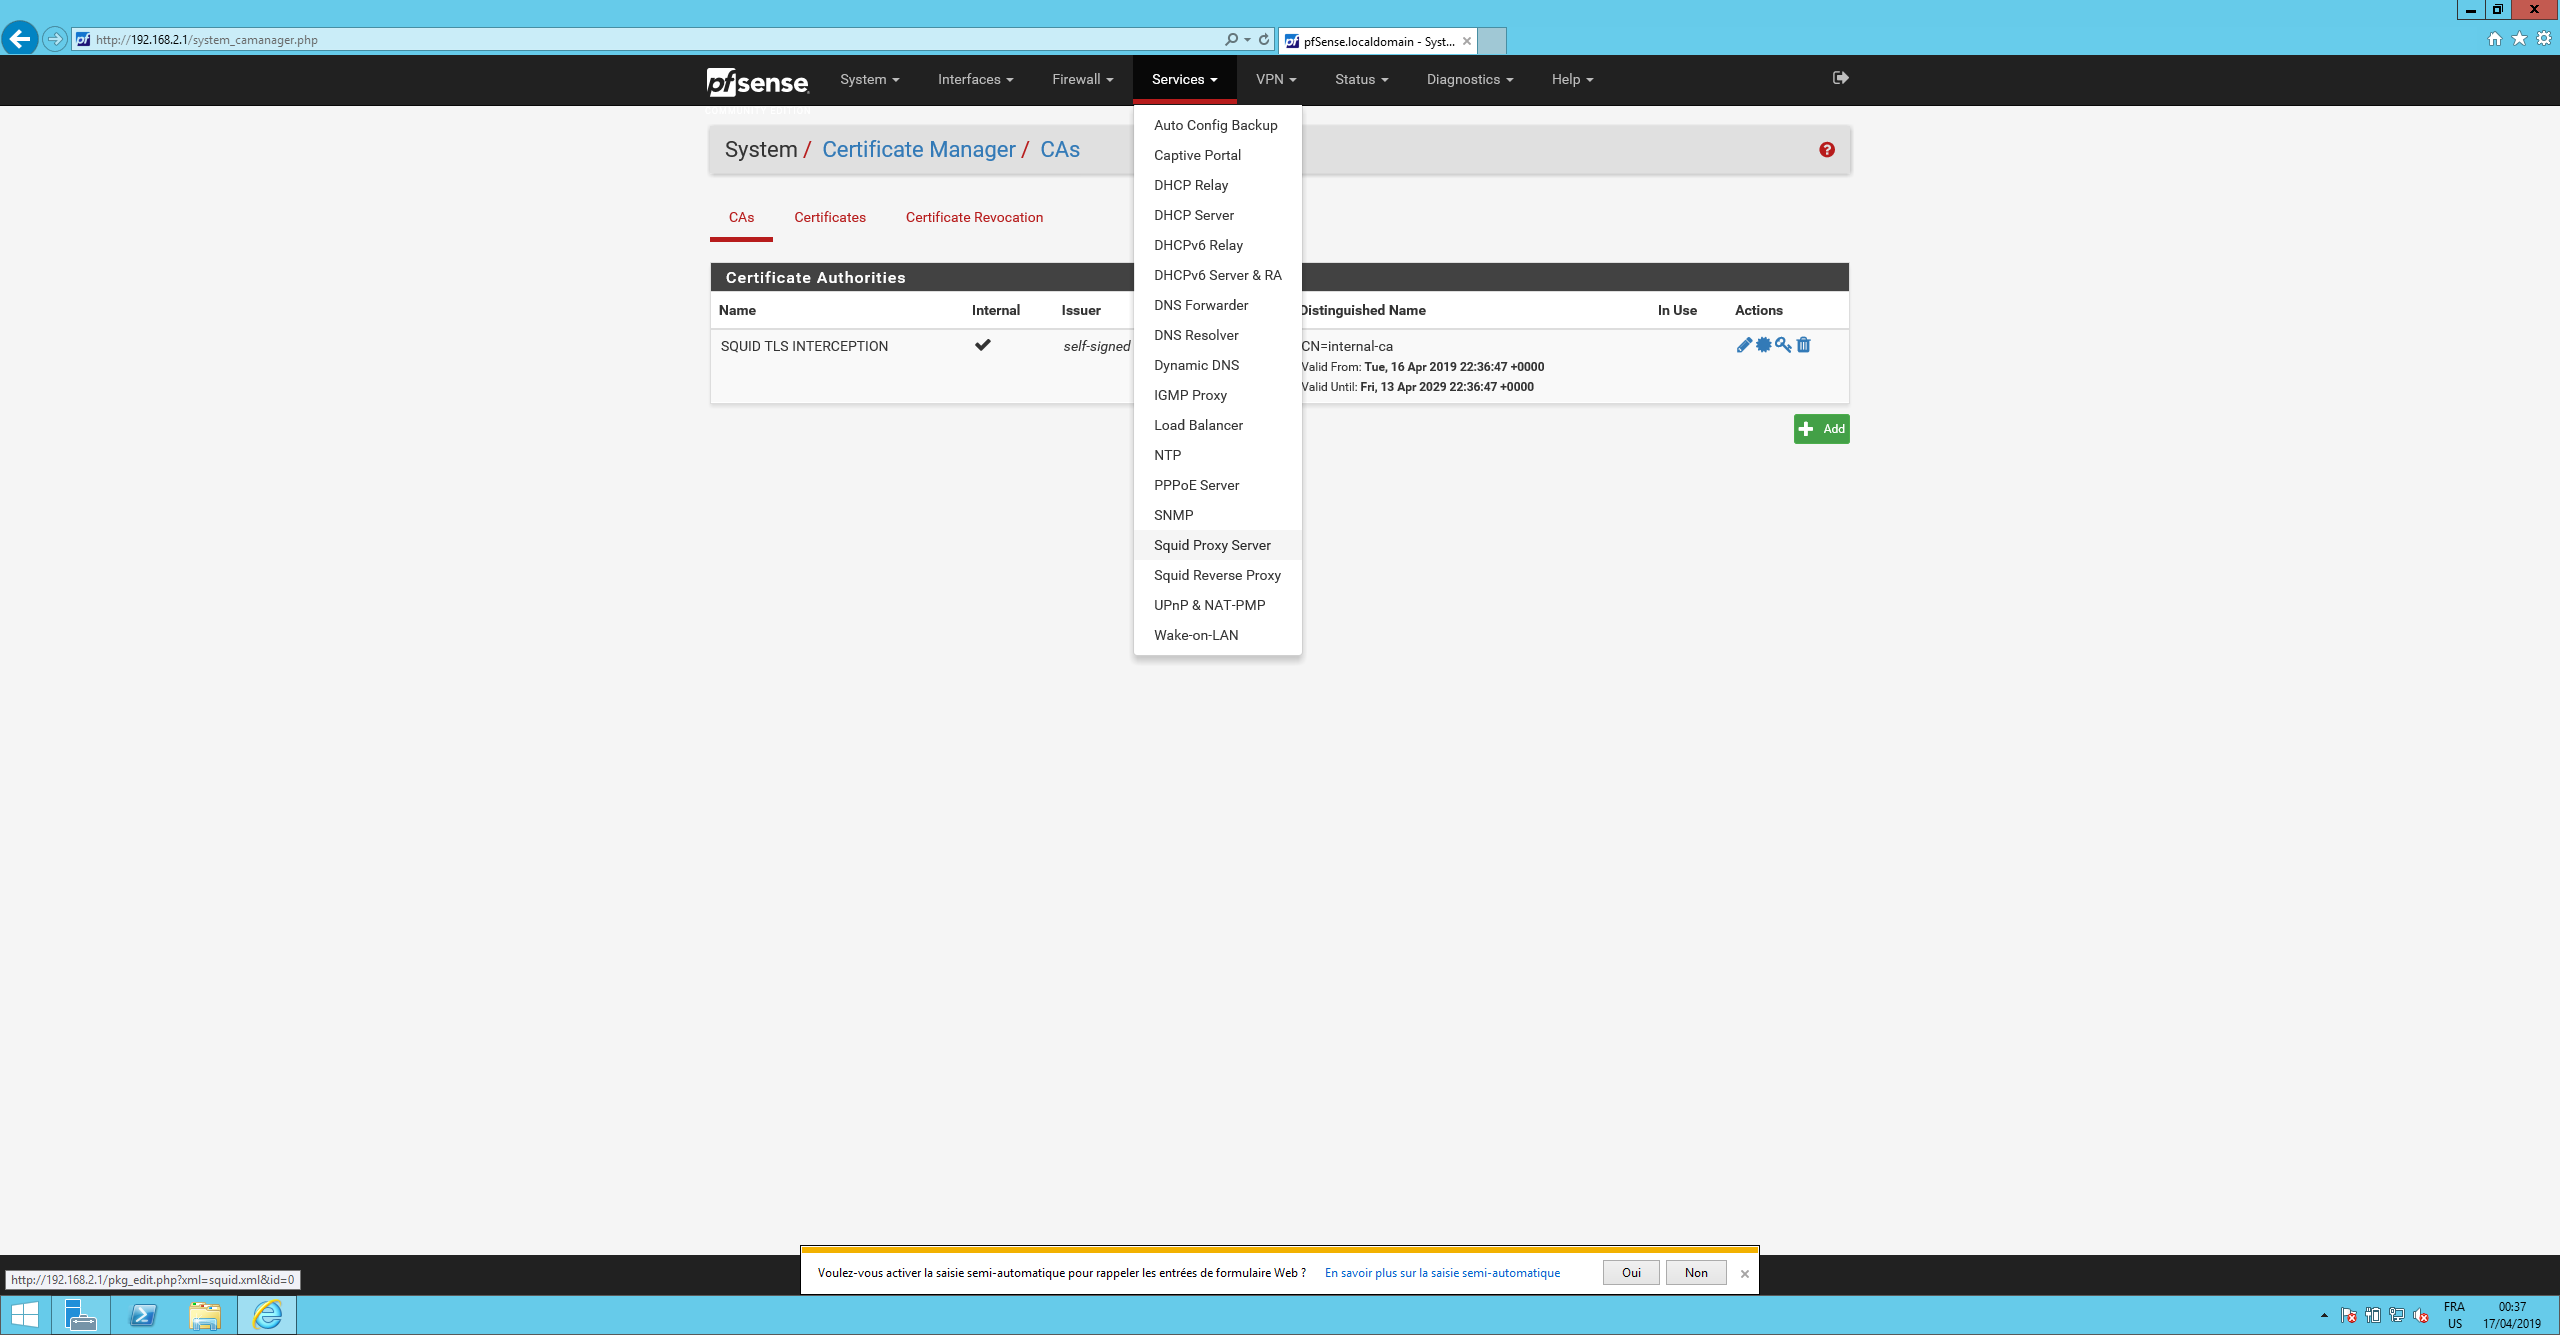
\includegraphics[scale=0.20]{Pfsense_Screeshots/interception/11.png}
        \label{Pfsense_Screeshots/interception/11}
        \caption{Accès au proxy Squid sur pfsense}
    \end{center}
\end{figure}
\FloatBarrier 
    
\item Changer la valeur du cache par \textit{500}, puis cliquer sur \textit{save} ;
\begin{figure}[h!]
    \begin{center}
        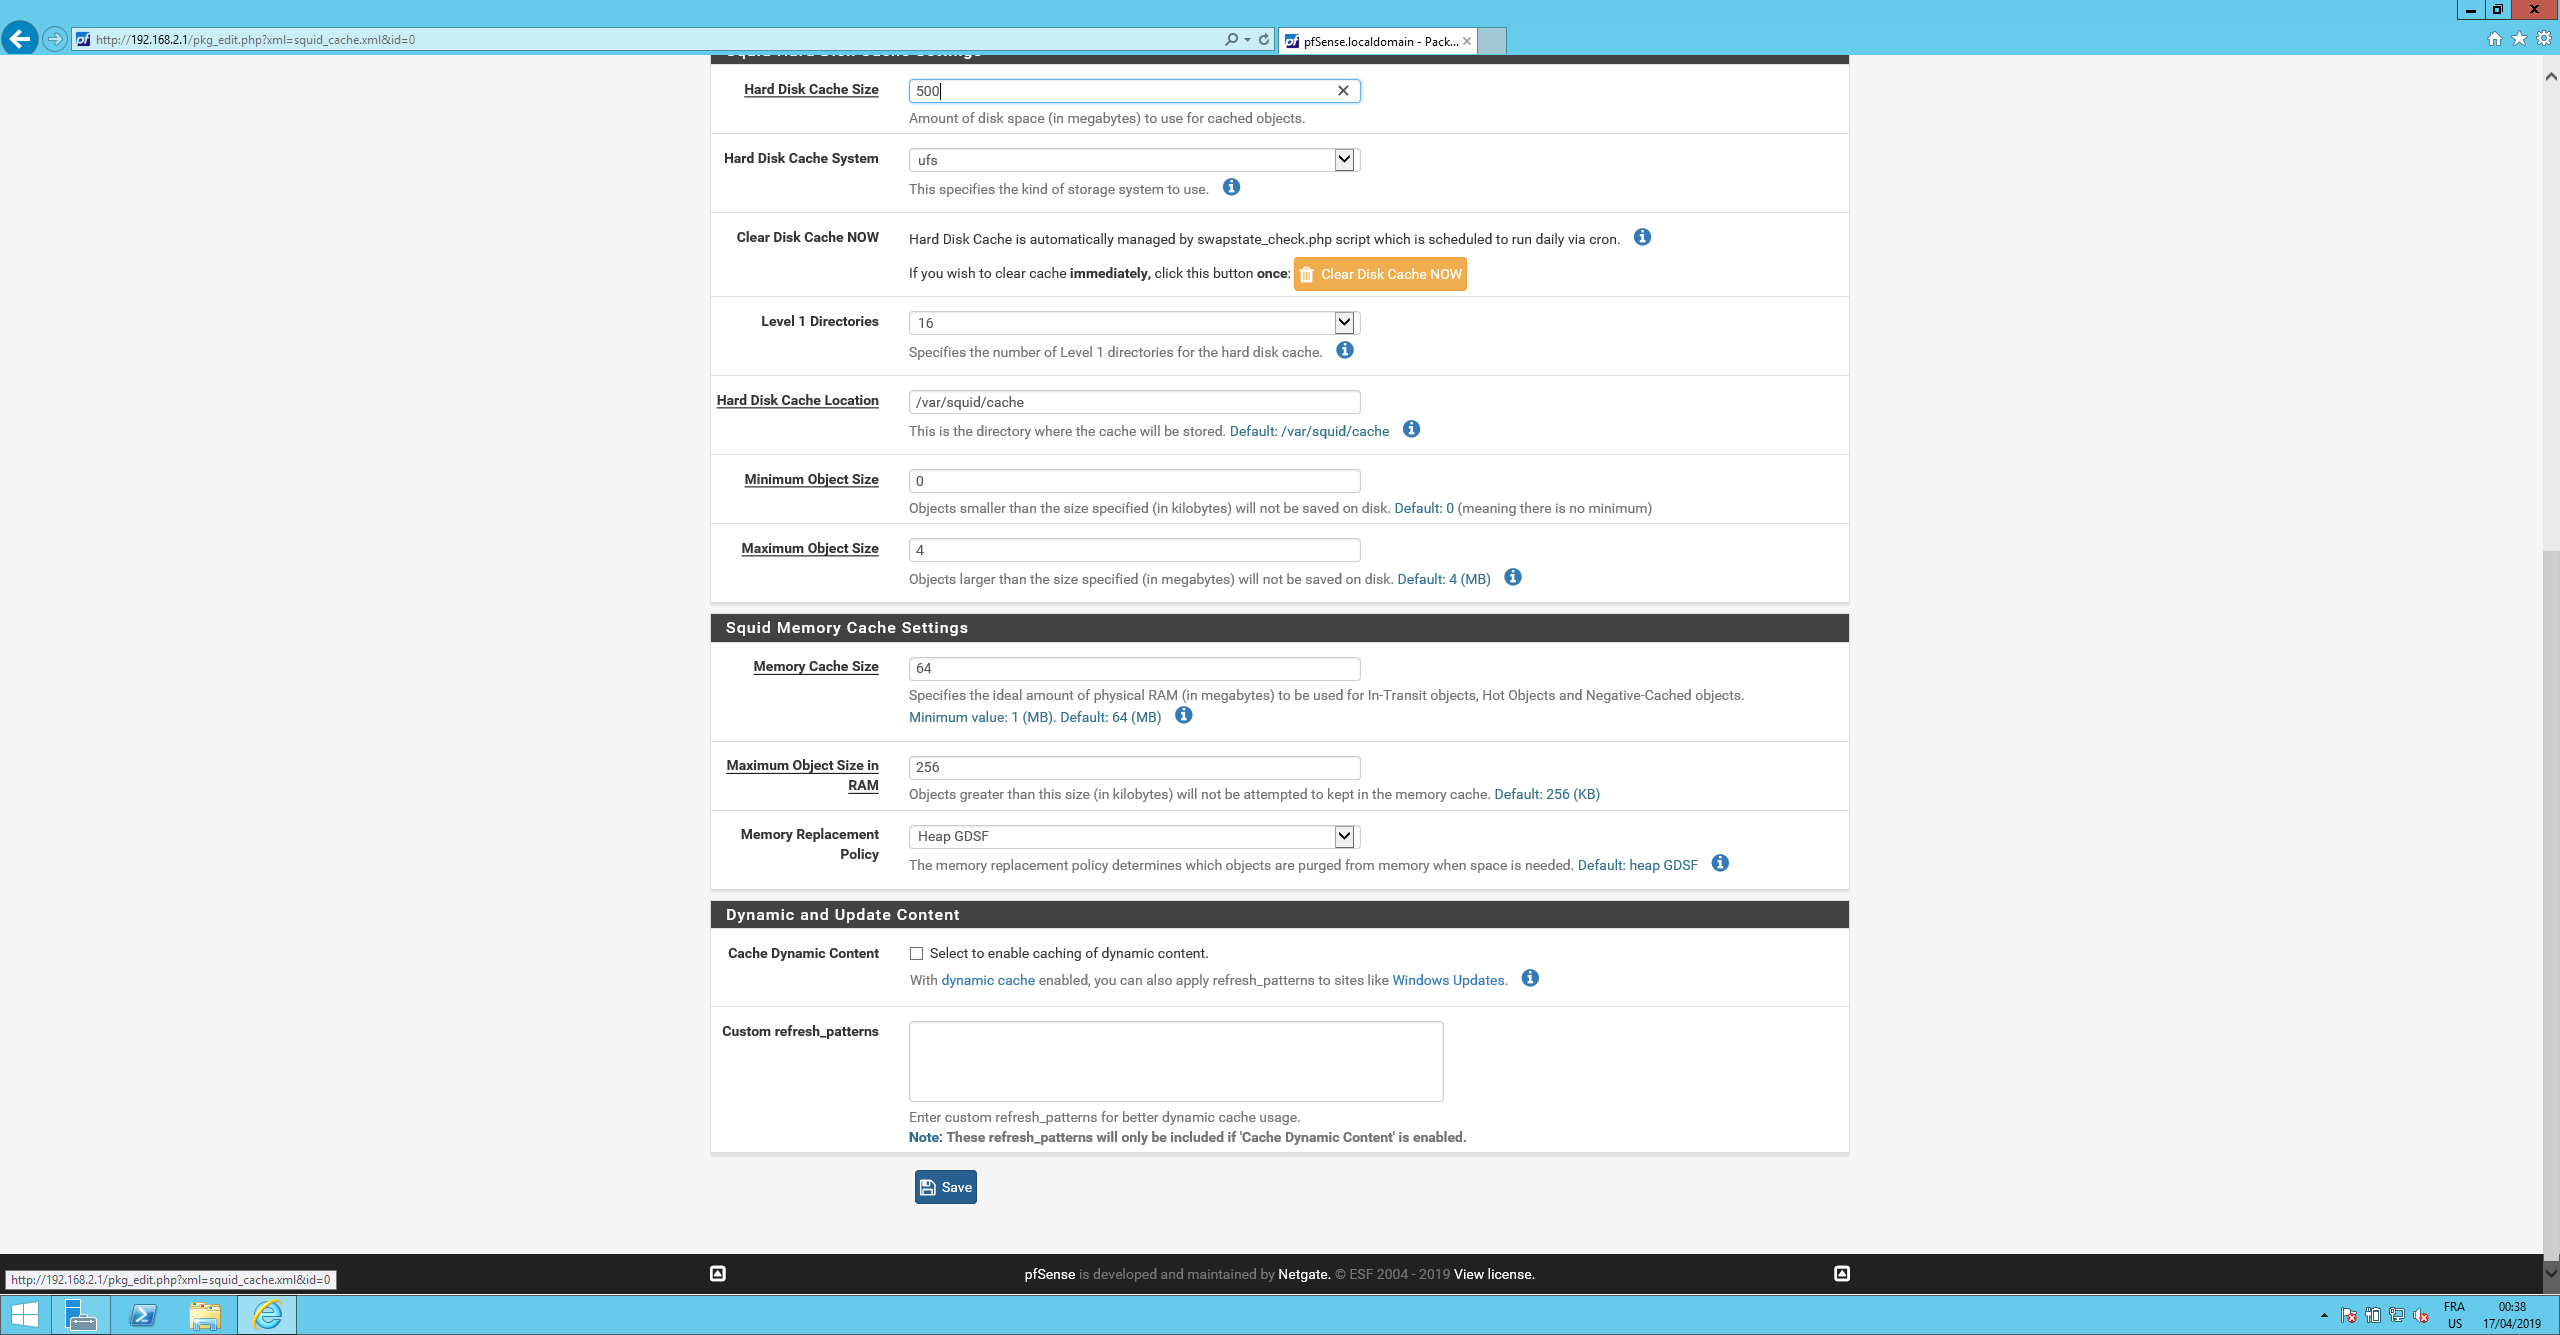
\includegraphics[scale=0.20]{Pfsense_Screeshots/interception/12.png}
        \label{Pfsense_Screeshots/interception/12}
        \caption{Modification du proxy Squid sur pfsense}
    \end{center}
\end{figure}
\FloatBarrier 
    
\item Cocher \textbf{Enable AV}, mettre \textbf{Enable Manual Configuration} à \textbf{enabled}, cliquer sur \textbf{Load Advanced} ;
\begin{figure}[h!]
    \begin{center}
        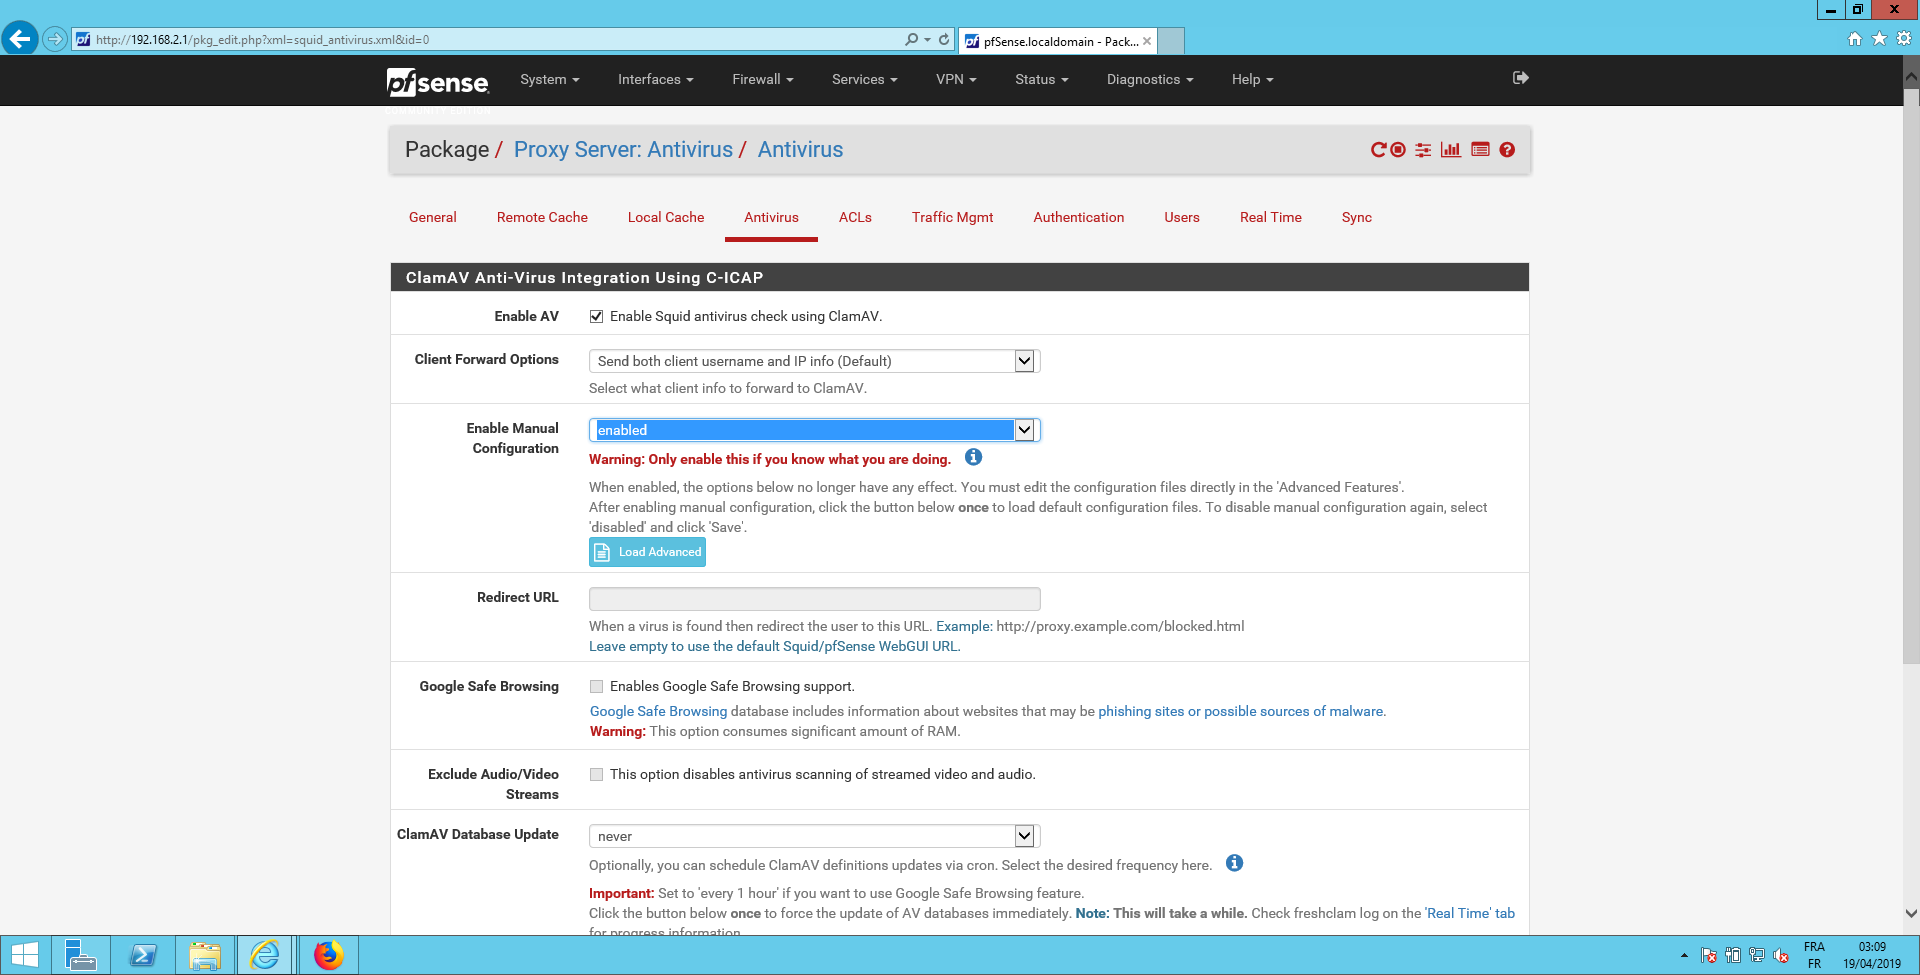
\includegraphics[scale=0.3]{Pfsense_Screeshots/interception/13.png}
        \label{Pfsense_Screeshots/interception/13}
        \caption{Initialisation de l'antivirus ClamAV sur pfsense}
    \end{center}
\end{figure}
\FloatBarrier 

\item Ouvrir la configuration avancée puis lire la valeur \textbf{DatabaseDirectory} dans \textbf{freshclam.conf}.
\begin{figure}[h!]
    \begin{center}
        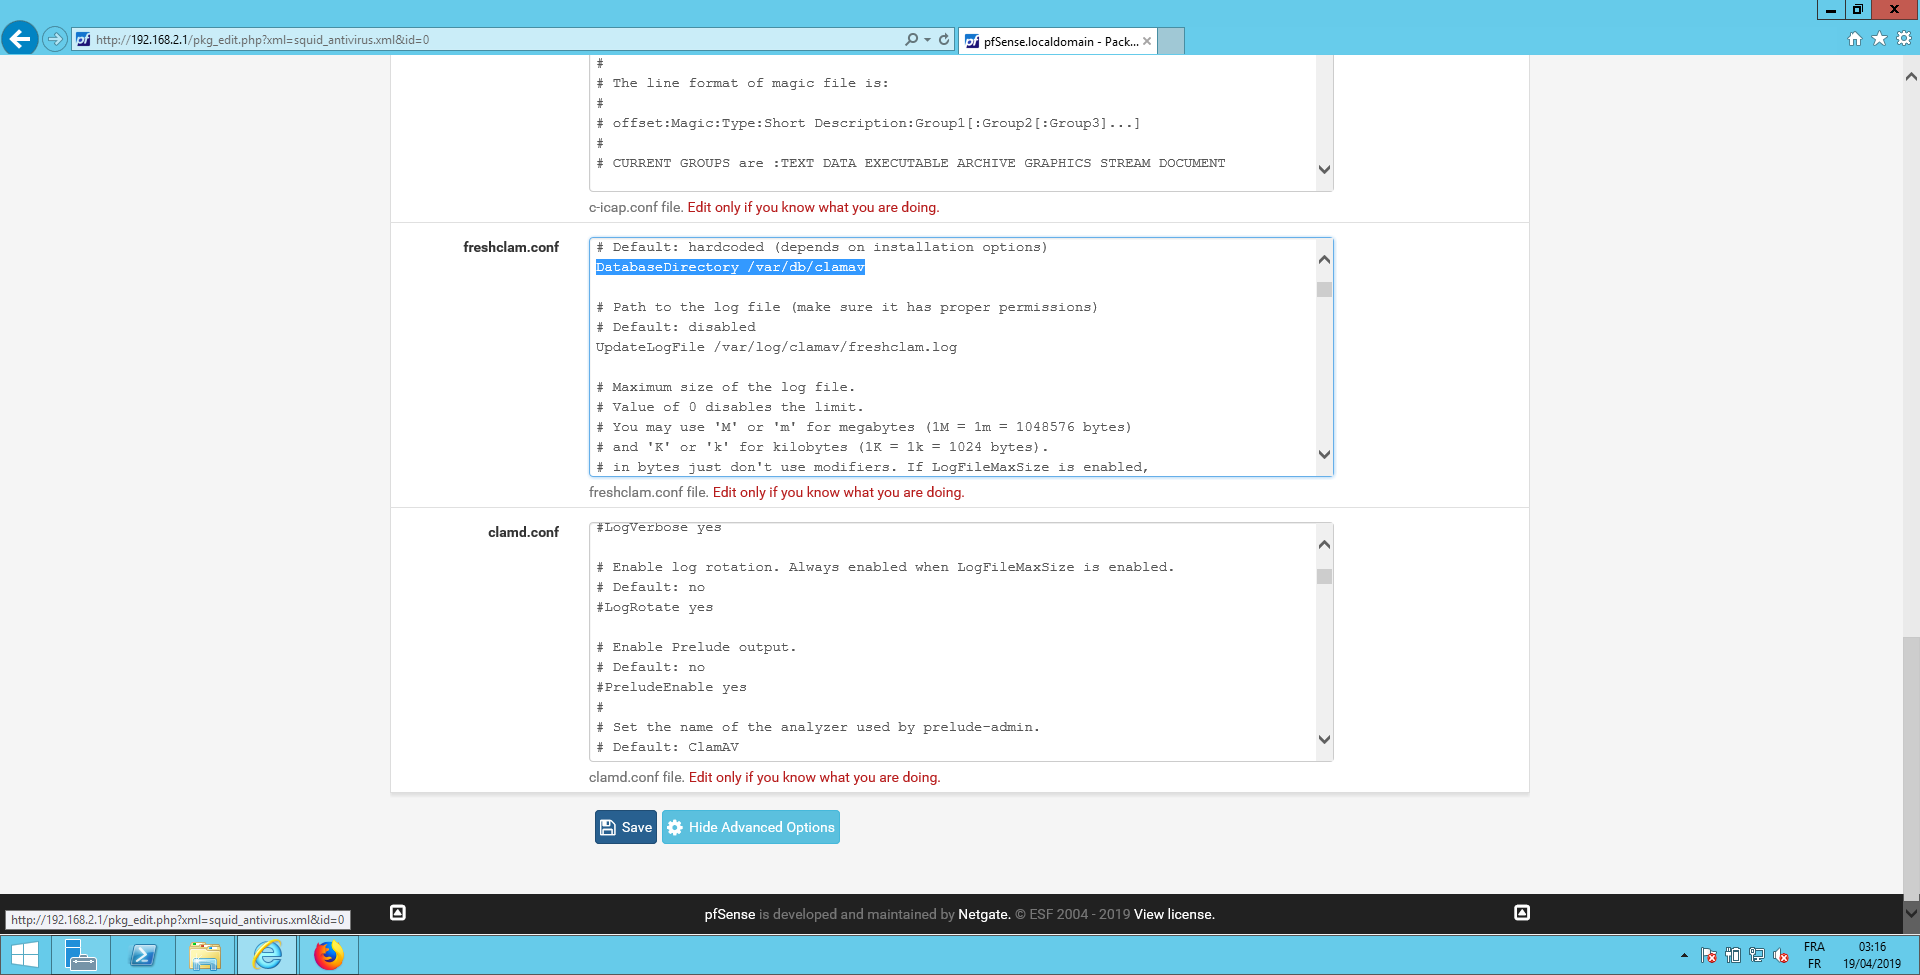
\includegraphics[scale=0.23]{Pfsense_Screeshots/interception/14.png}
        \label{Pfsense_Screeshots/interception/14}
        \caption{Lecture de la valeur dans freshclam.conf sur pfsense}
    \end{center}
\end{figure}
\FloatBarrier 

\end{itemize}

\begin{itemize}
   \item Accéder à \textbf{Services -> Squid Proxy Server} ;
   \item Cocher \textbf{Enable Squid Proxy}, cocher \textbf{Keep Settings/Data}, mettre \textbf{Proxy Interface(s)} à \textbf{LAN}, cliquer sur \textbf{Load Advanced} ;
   \item Cocher \textbf{Transparent HTTP Proxy} ;
\begin{figure}[h!]
    \begin{center}
        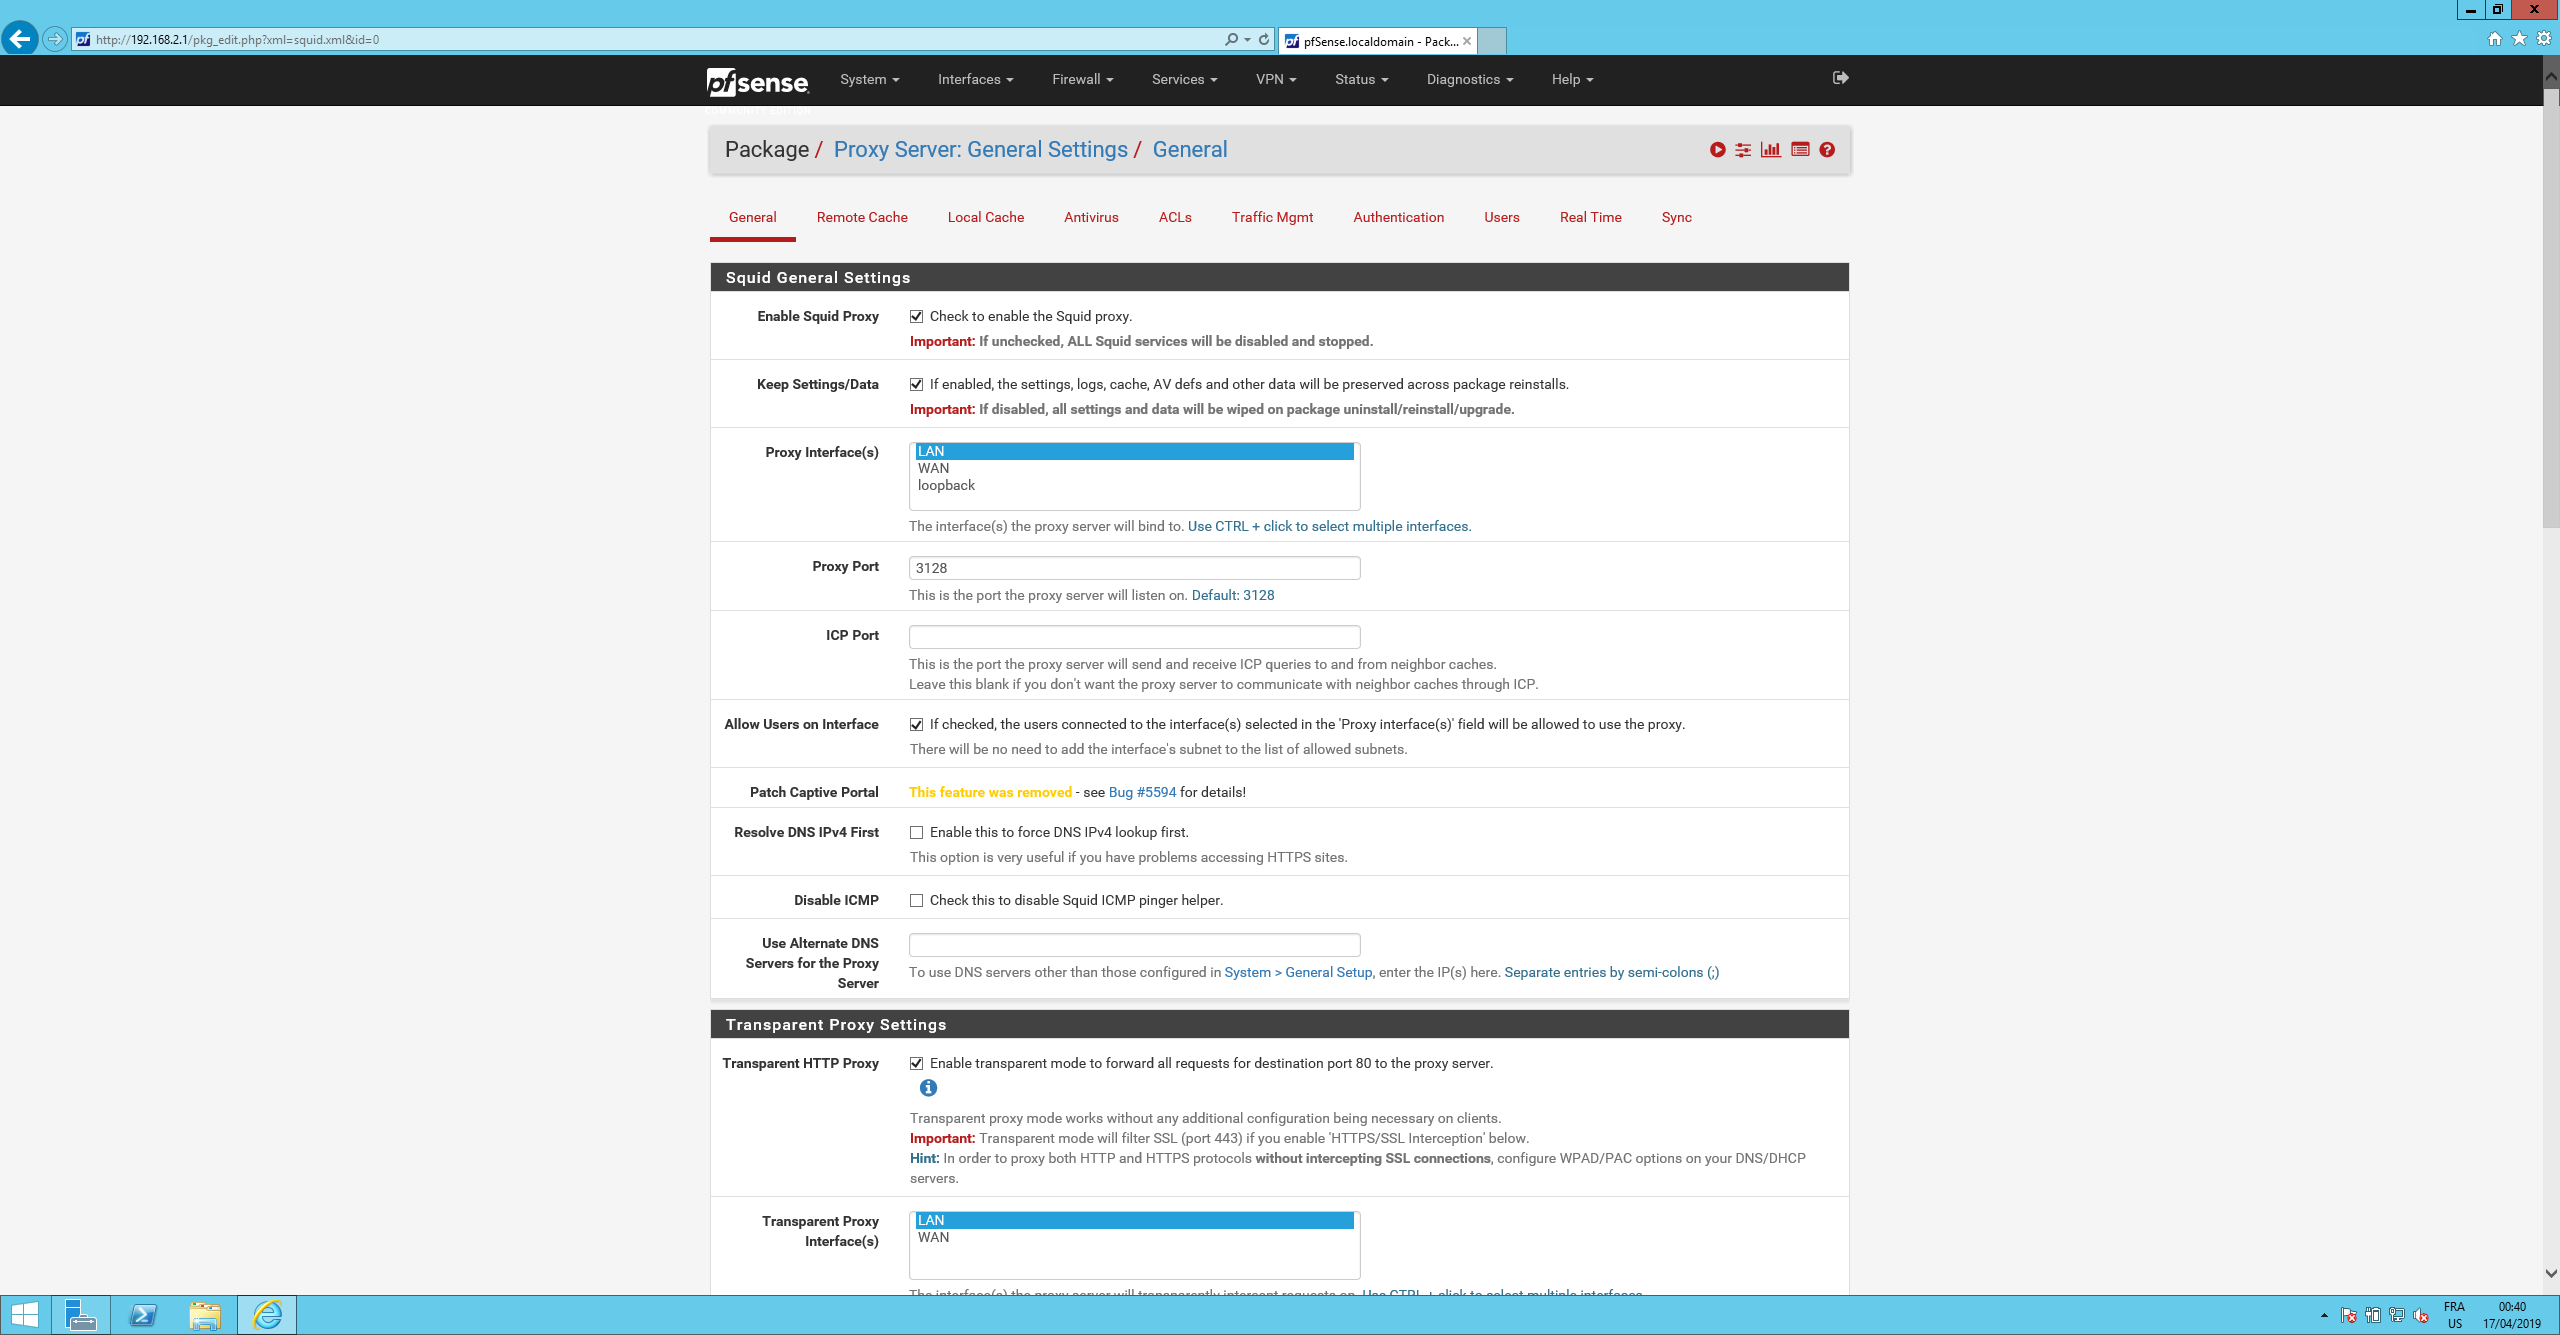
\includegraphics[scale=0.20]{Pfsense_Screeshots/interception/15.png}
        \label{Pfsense_Screeshots/interception/15}
        \caption{Paramétrage du proxy Squid sur pfsense}
    \end{center}
\end{figure}
\FloatBarrier 
    
    \item Cocher \textbf{HTTPS/SSL Interception} ;
    \item Cocher \textbf{Enable Access Logging} ;
    \item Cliquer sur \textbf{save} ;
\begin{figure}[h!]
    \begin{center}
        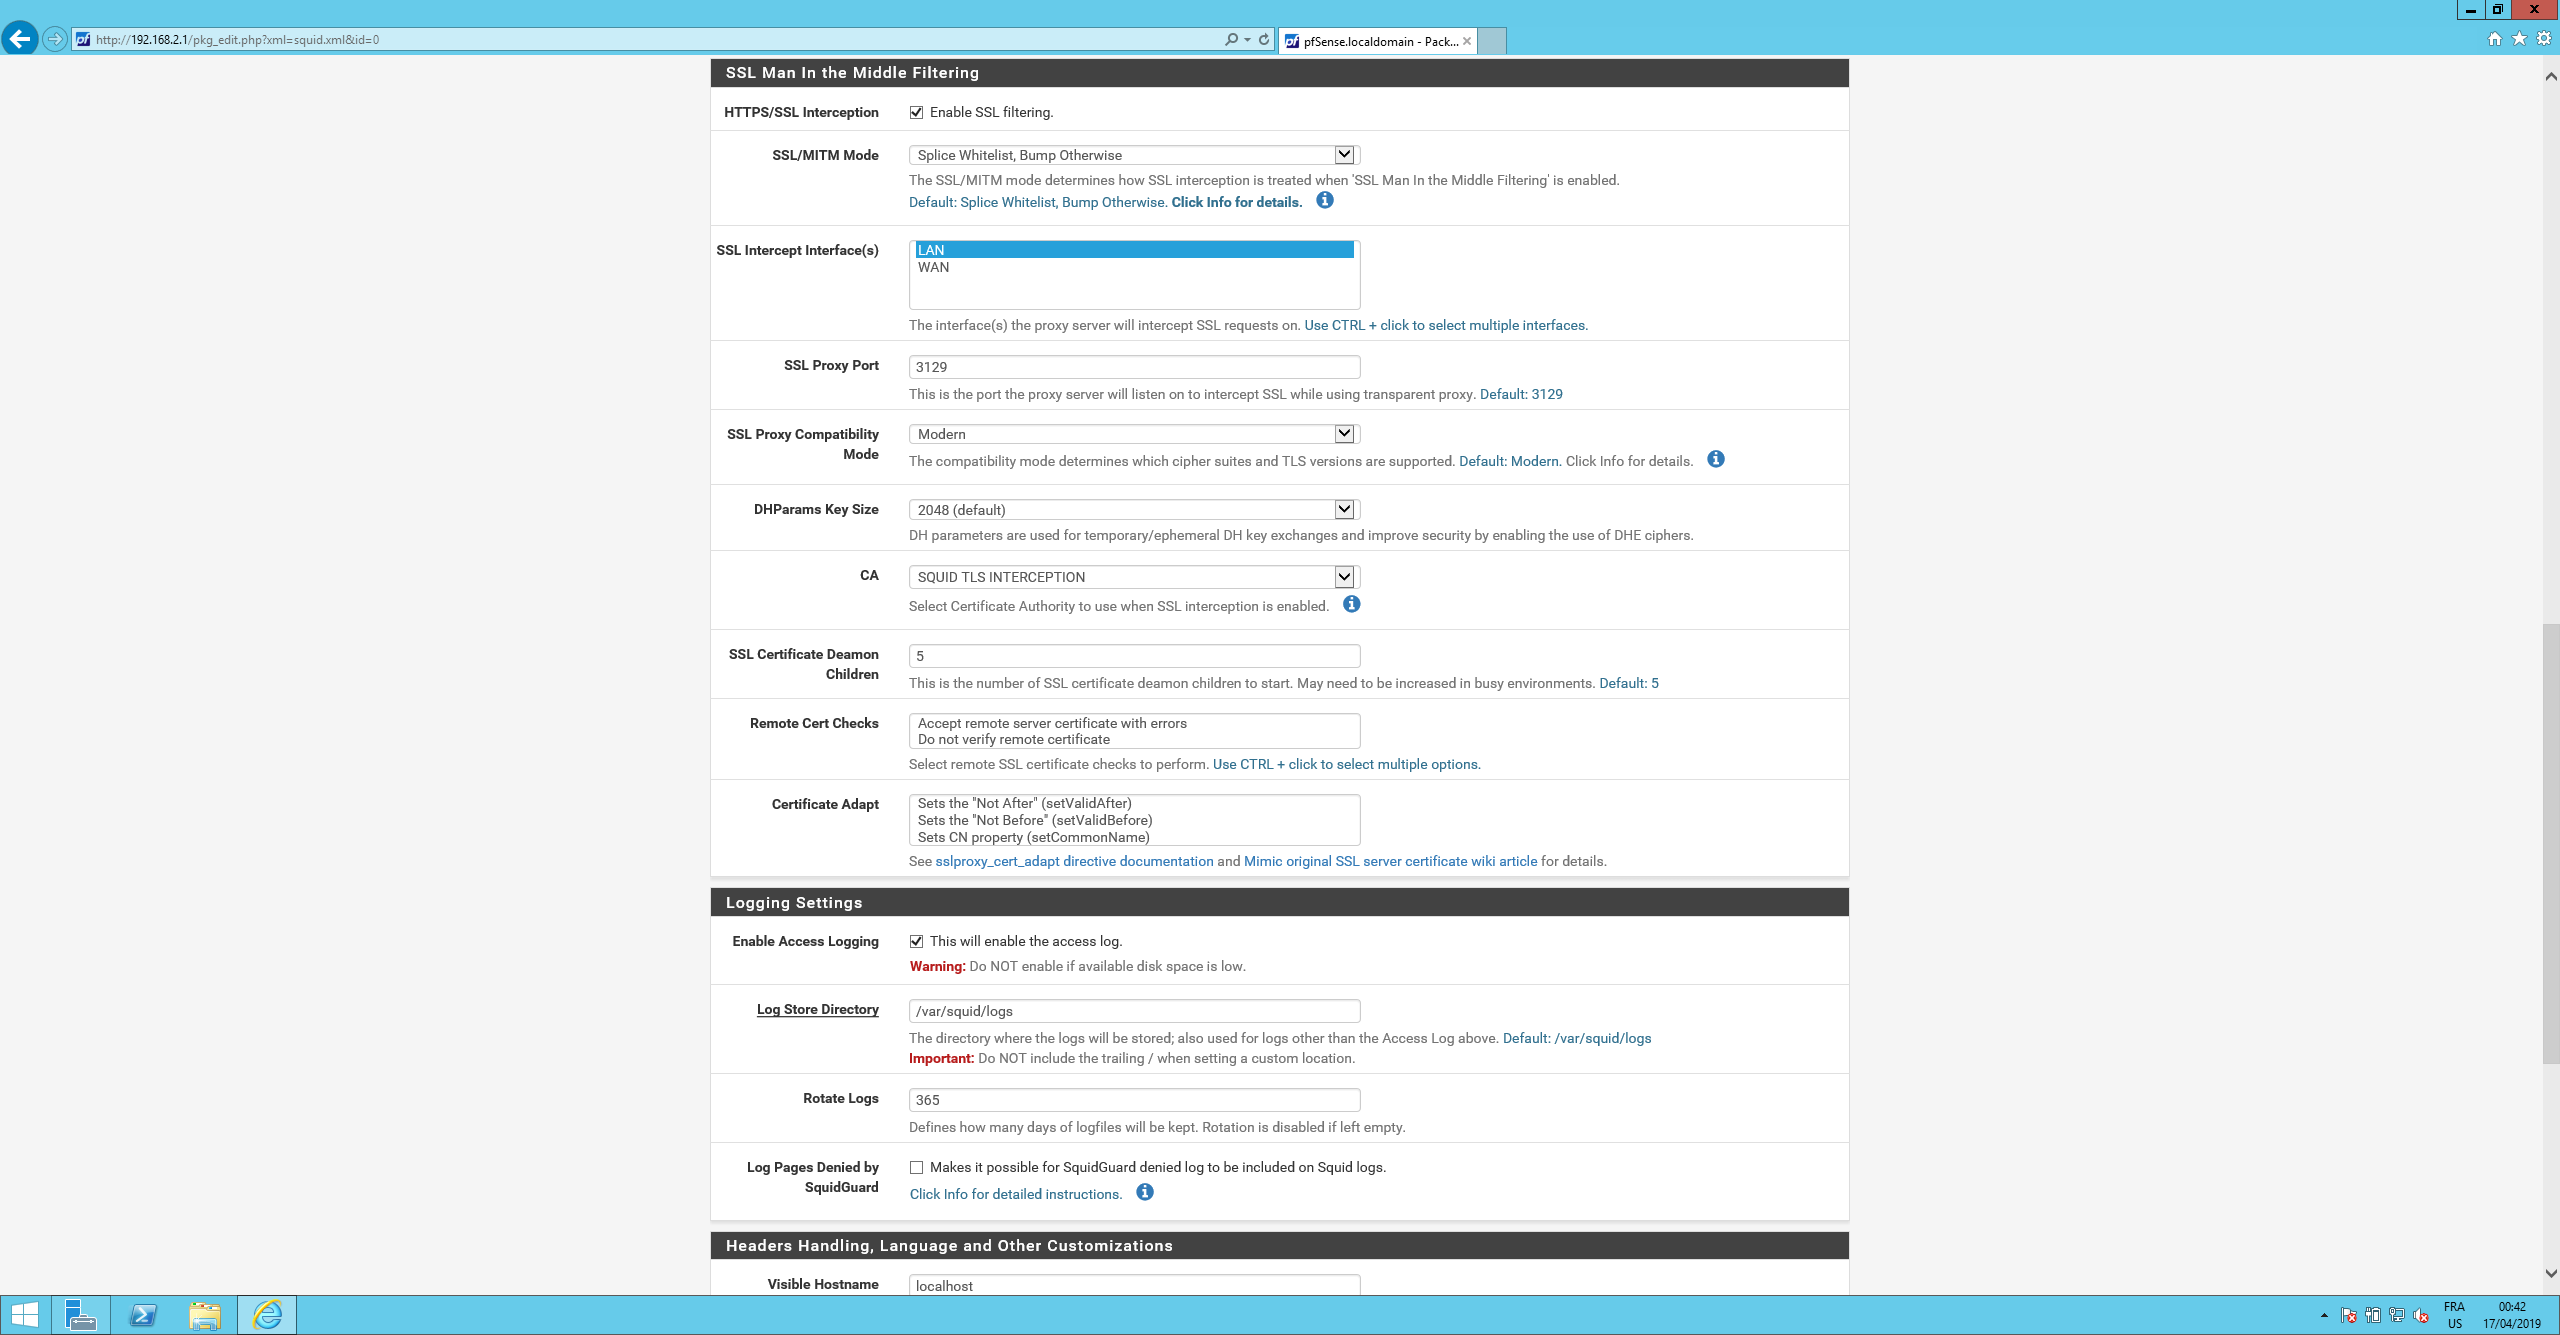
\includegraphics[scale=0.20]{Pfsense_Screeshots/interception/16.png}
        \label{Pfsense_Screeshots/interception/16}
        \caption{Paramétrage du HTTPS/SSL de Squid sur pfsense}
    \end{center}
\end{figure}
\FloatBarrier 
    
\item Comme fait précédemment, ajouter une règle sur pfsense ;
\begin{figure}[h!]
    \begin{center}
        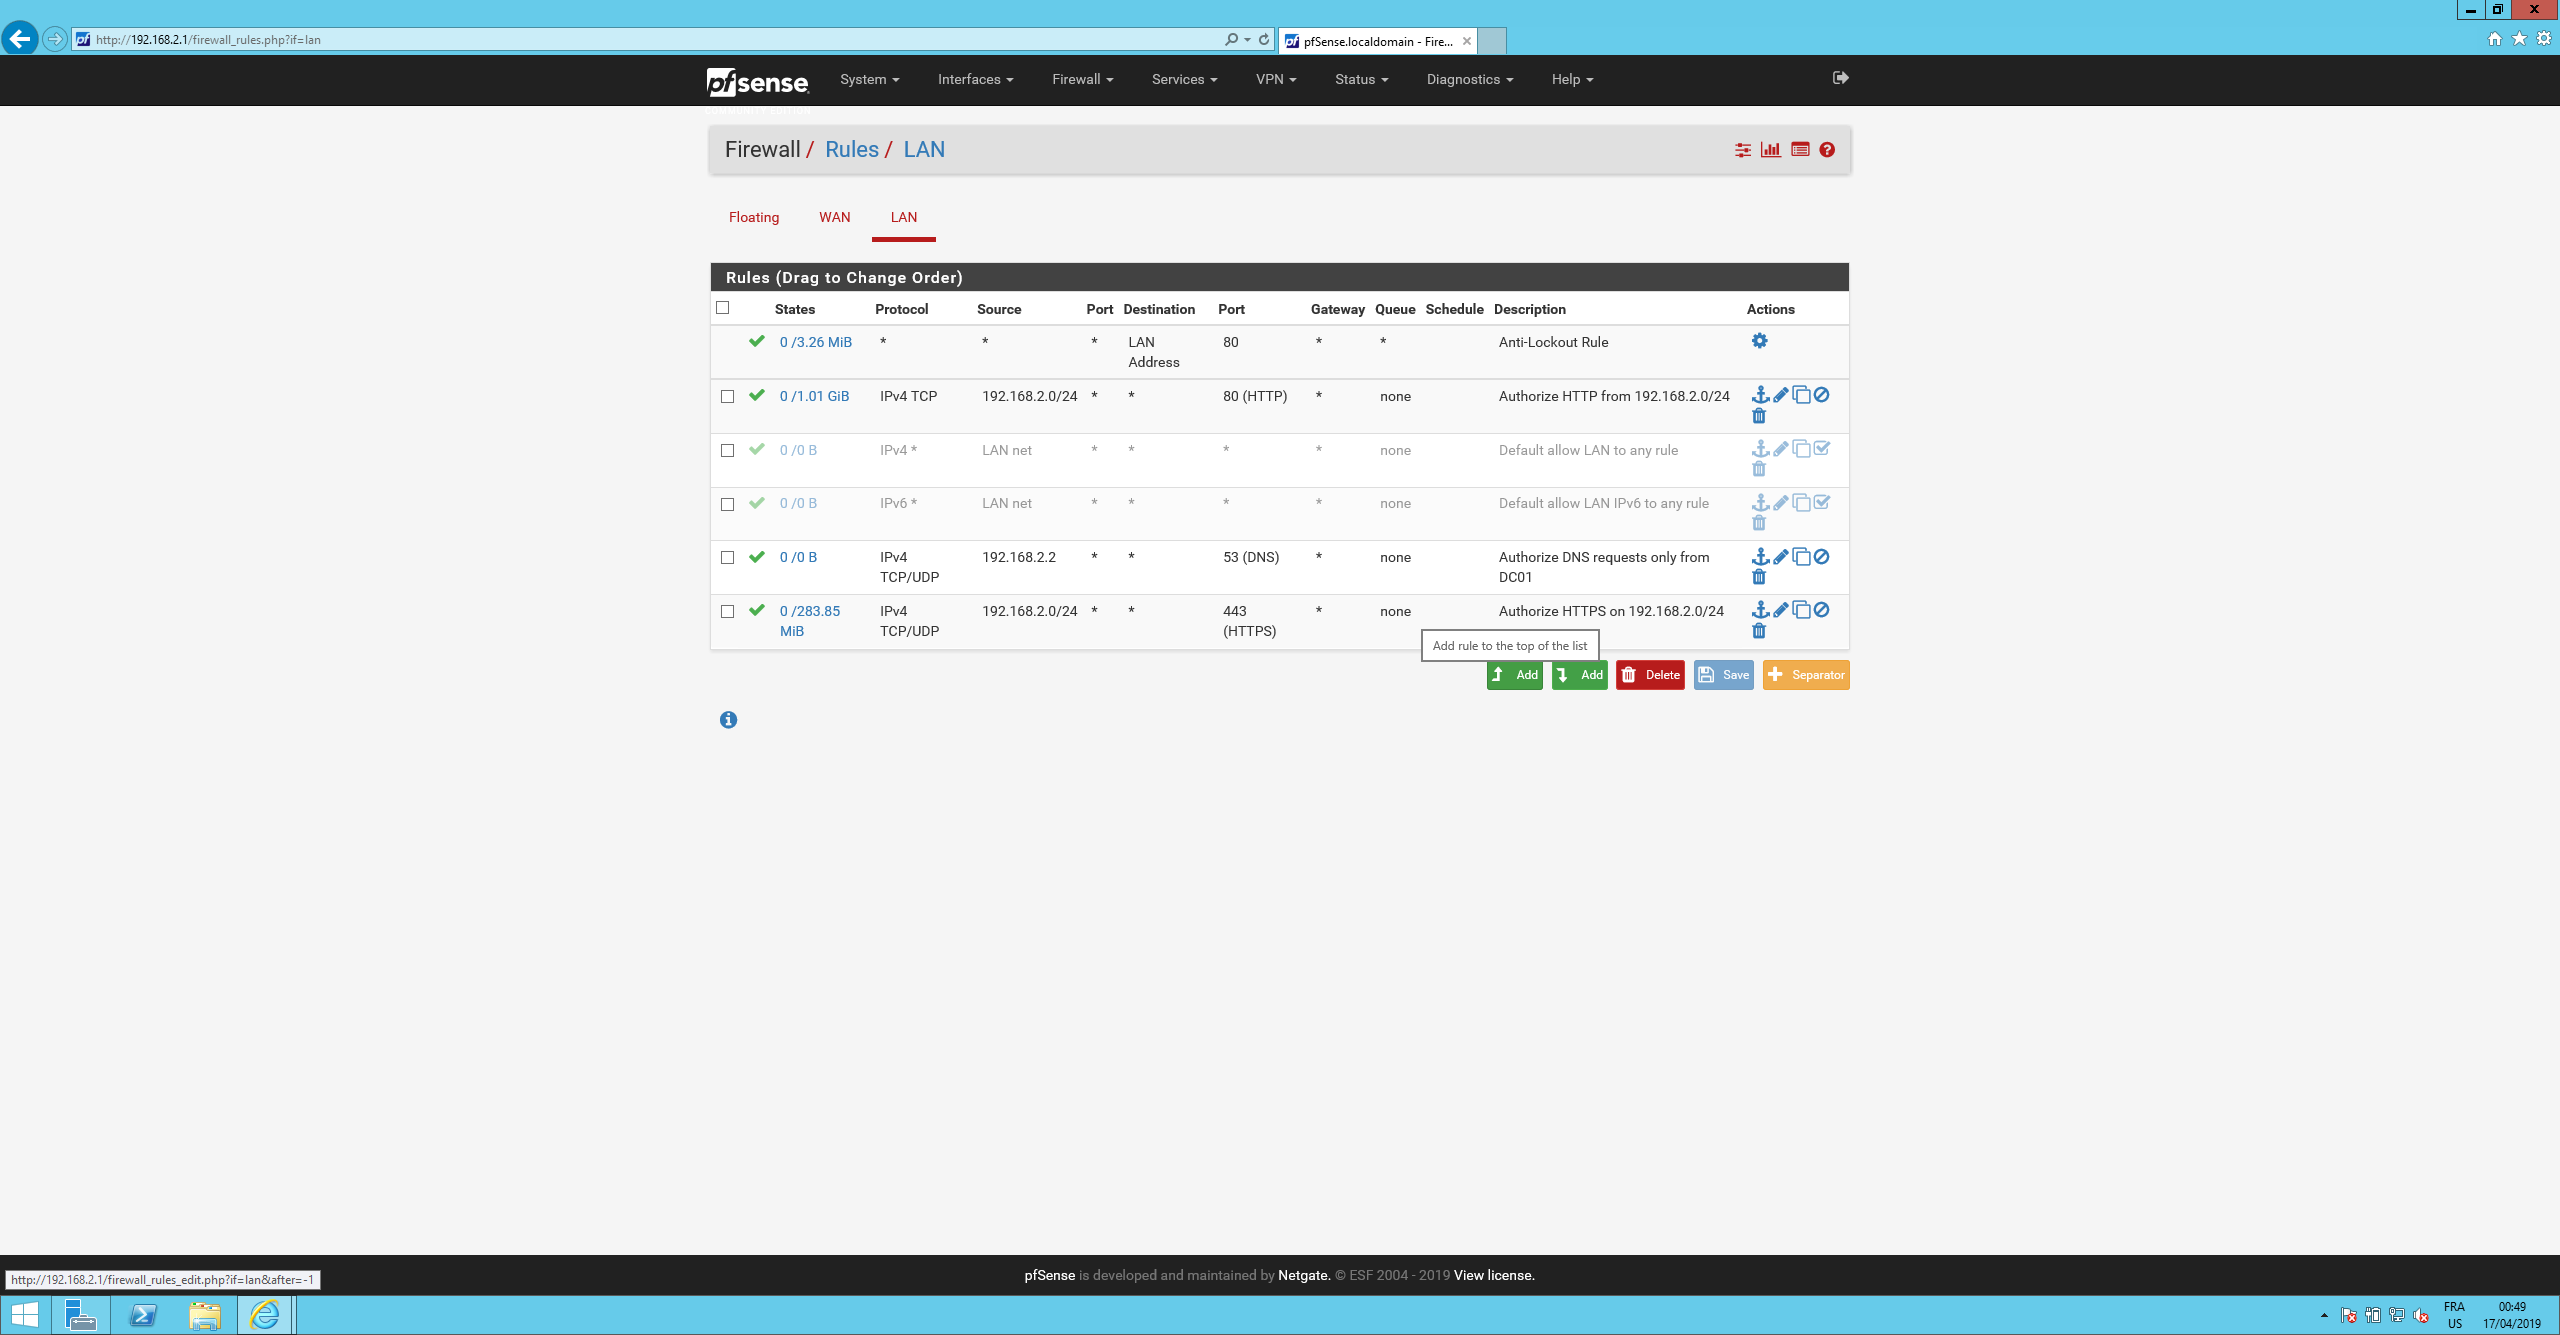
\includegraphics[scale=0.20]{Pfsense_Screeshots/interception/17.png}
        \label{Pfsense_Screeshots/interception/17}
        \caption{Ajout d'une règle à pfsense}
    \end{center}
\end{figure}
\FloatBarrier 
    
\item Paramétrer la configuration pour autoriser les ports 3128 et 3129, puis cliquer sur \textit{save};
\begin{figure}[h!]
    \begin{center}
        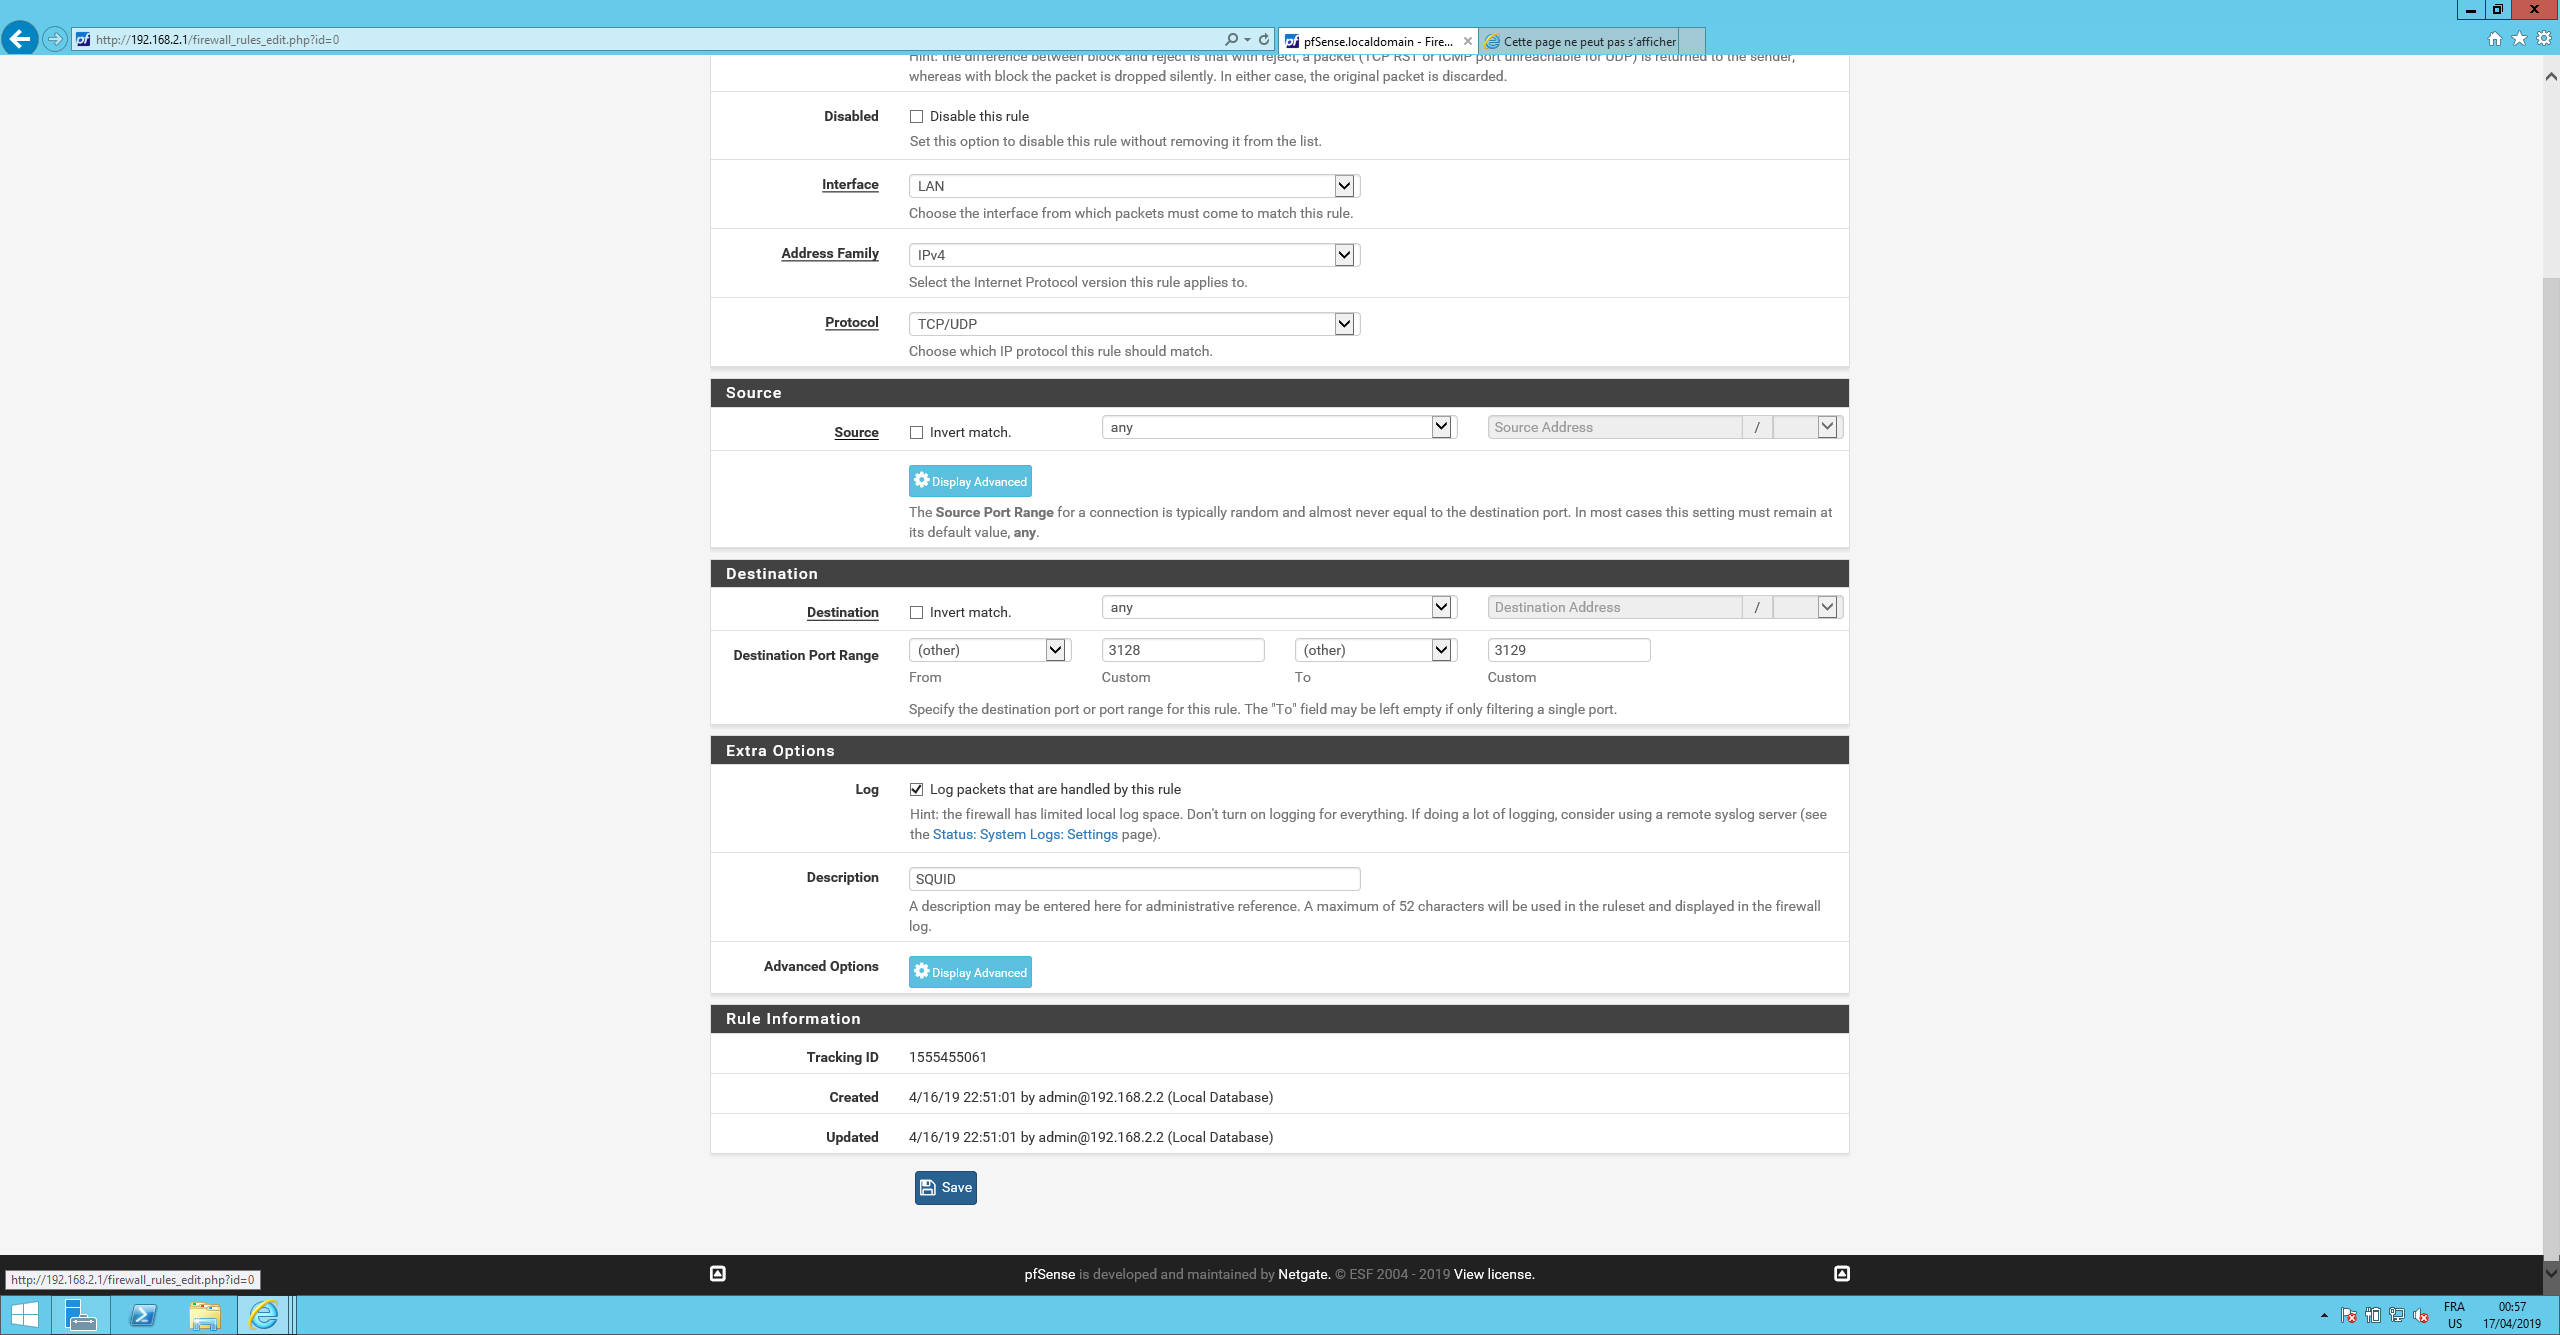
\includegraphics[scale=0.20]{Pfsense_Screeshots/interception/18.png}
        \label{Pfsense_Screeshots/interception/18}
        \caption{Paramétrage de la règle sur pfsense}
    \end{center}
\end{figure}
\FloatBarrier 

\item Pour interdire tous les navigateurs sauf Internet Explorer en version supérieure à 10, il faut ajouter la regex présentée ci-dessous dans l'onglet \textbf{ACLs}, à \textbf{Block User Agents}.
\begin{figure}[h!]
    \begin{center}
        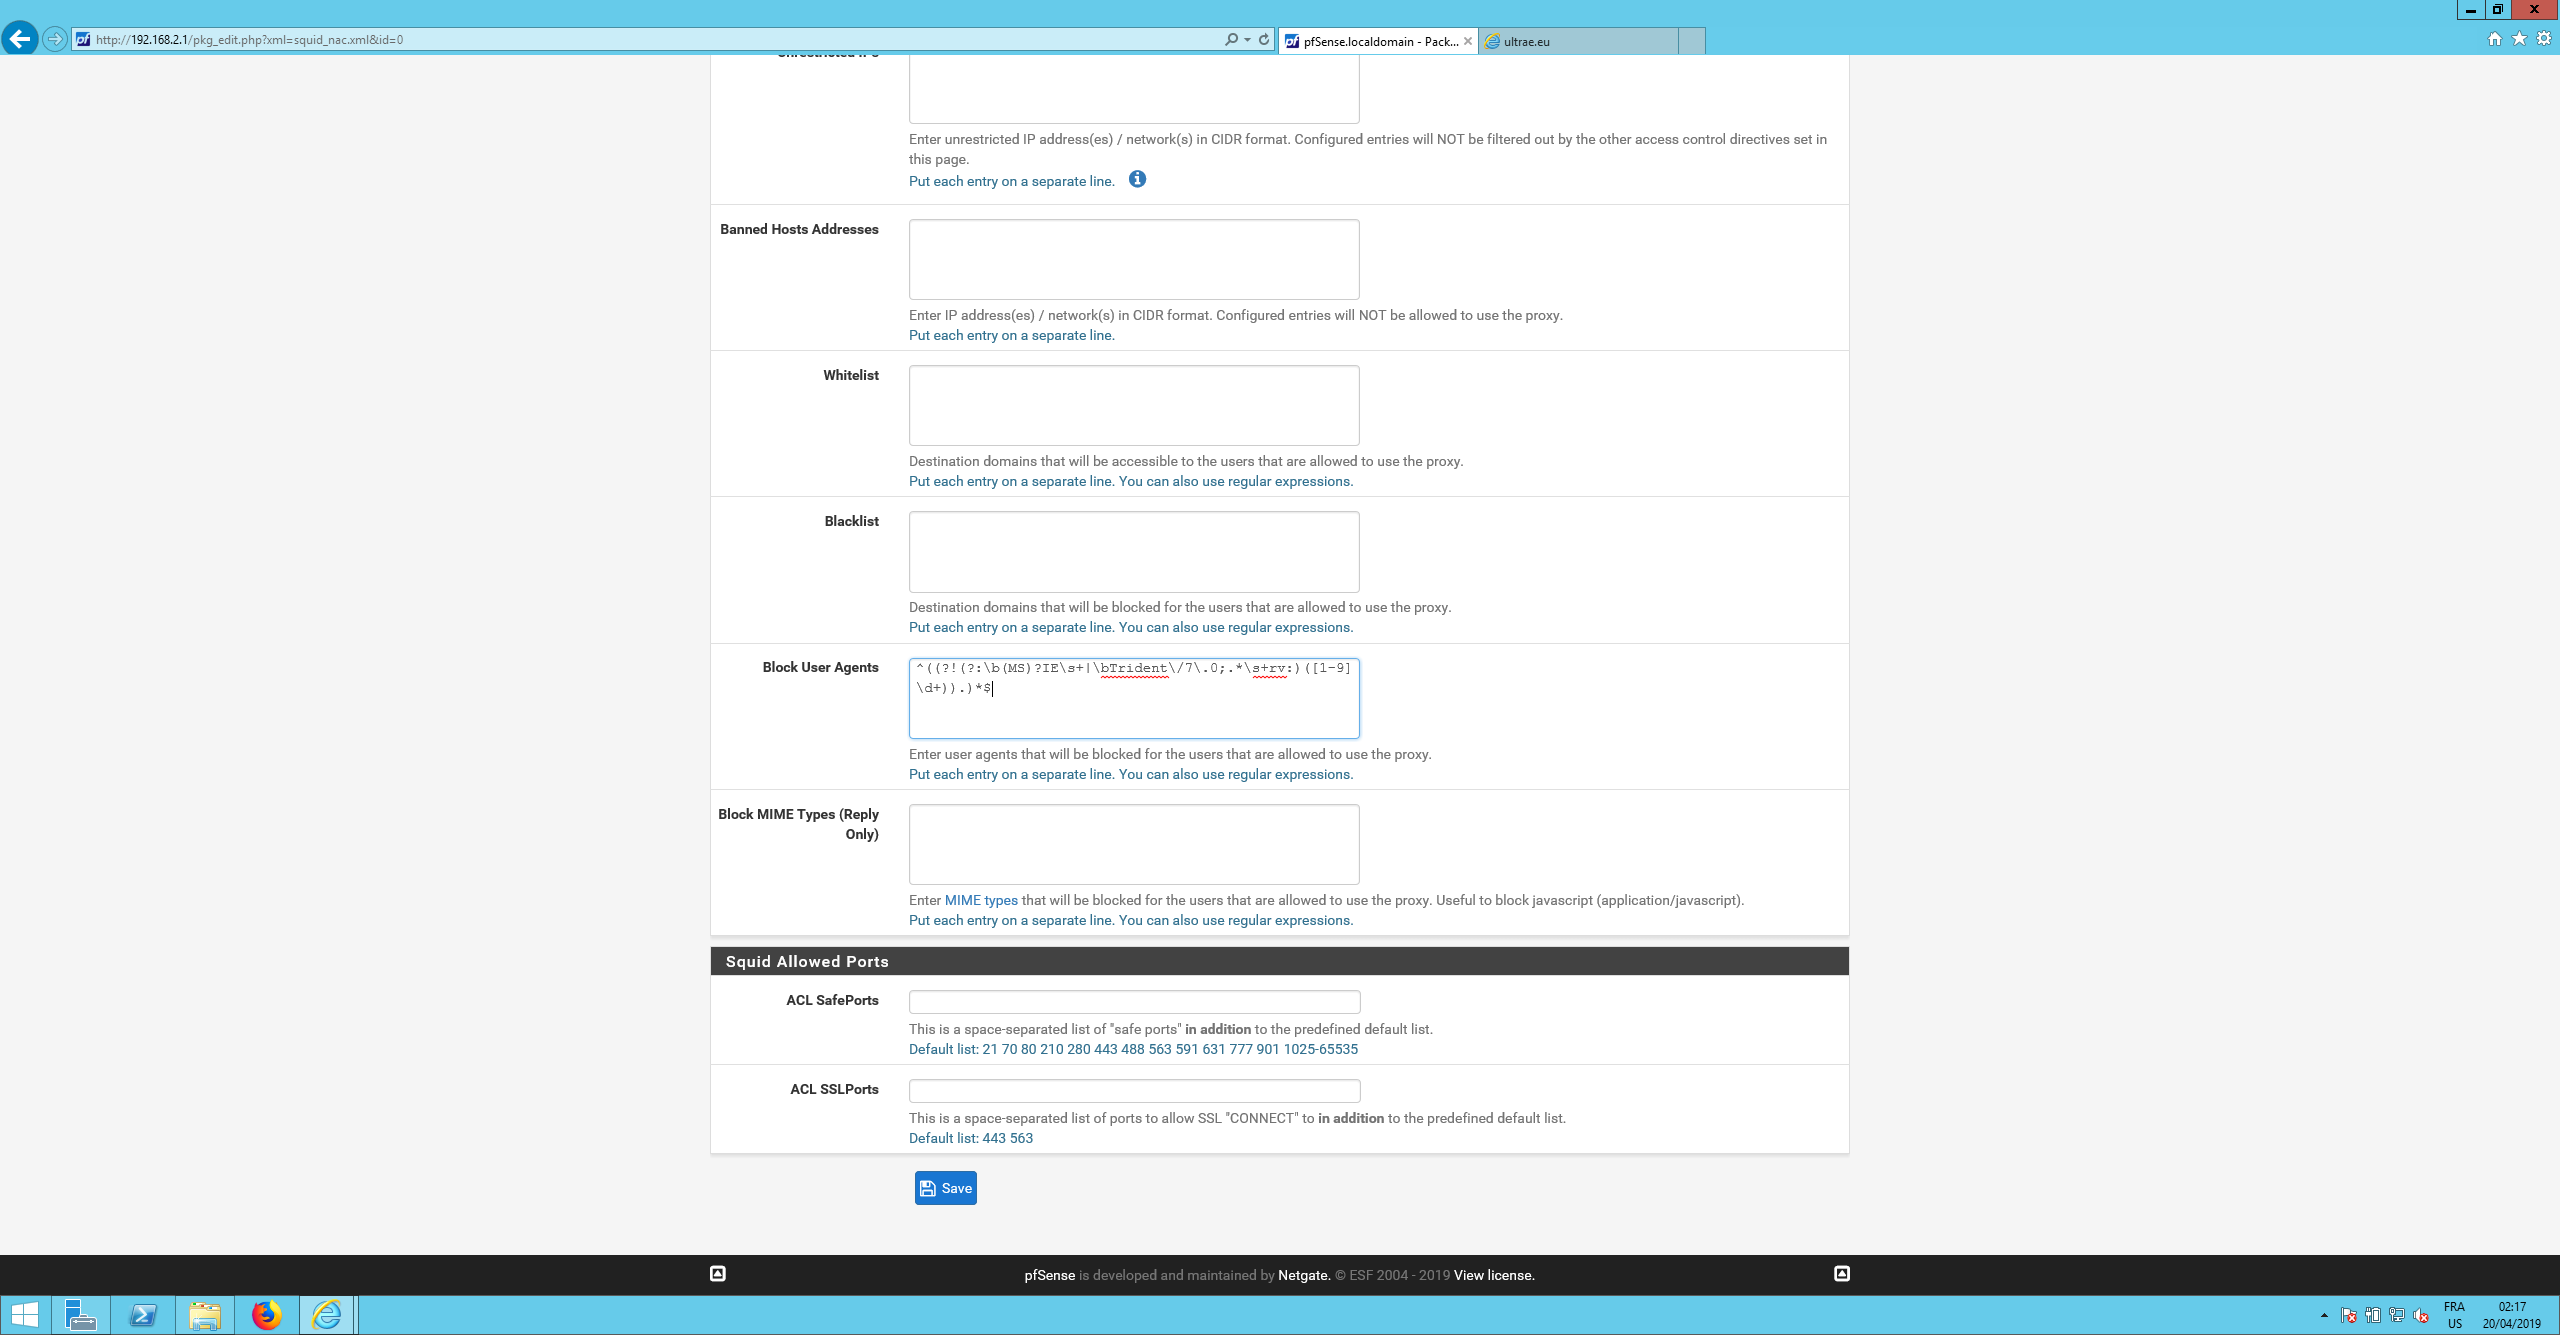
\includegraphics[scale=0.20]{Pfsense_Screeshots/interception/19.png}
        \label{Pfsense_Screeshots/interception/19}
        \caption{Restriction du navigateur sur pfsense}
    \end{center}
\end{figure}
\FloatBarrier 
\end{itemize}
\newpage

\subsection{Filtrage du mot clé EPITA via ClamAV}

Pour pouvoir filtrer tous les paquets contenant le mot clé \textbf{EPITA} avec \textit{SQUID}, nous utiliserons l'anti-virus intégré : \textit{ClamAV}. \\

Lorsque clamAV détecte une page web en entrée, à l'aide d'une balise HTML valide, il se comporte comme suit \cite{Clamav-signatures} :
\begin{enumerate}
    \item le fichier est normalisé, les commentaires sont supprimés, tout est mis en minuscule et les espaces en trop sont supprimés ;
    \item les tags HTML sont enlevés ;
    \item un fichier contenant le javascript est créé.
\end{enumerate}

Nous cherchons donc à créer une signature permettant de détecter le mot clé \textbf{EPITA} et donc nous notifier.
Pour cela, plusieurs formats se présentent à nous. Nous en retiendrons deux :
\begin{itemize}
    \item les \textit{.yara} \cite{yara-signatures} \cite{yara-hunting-signatures};
    \item les \textit{.ndb}\cite{ndb-signatures}.
\end{itemize}

Ainsi, après avoir lu où se trouve les signatures de \textit{ClamAV} via les fichiers de configuration de \textit{SQUID}, nous rajouterons les notres (voir dev.pdf pour le contenu) dans le dossier adéquat.

Ci-dessous, le résultat après une recherche google avec des termes proches d'epita.
\begin{figure}[h!]
    \begin{center}
        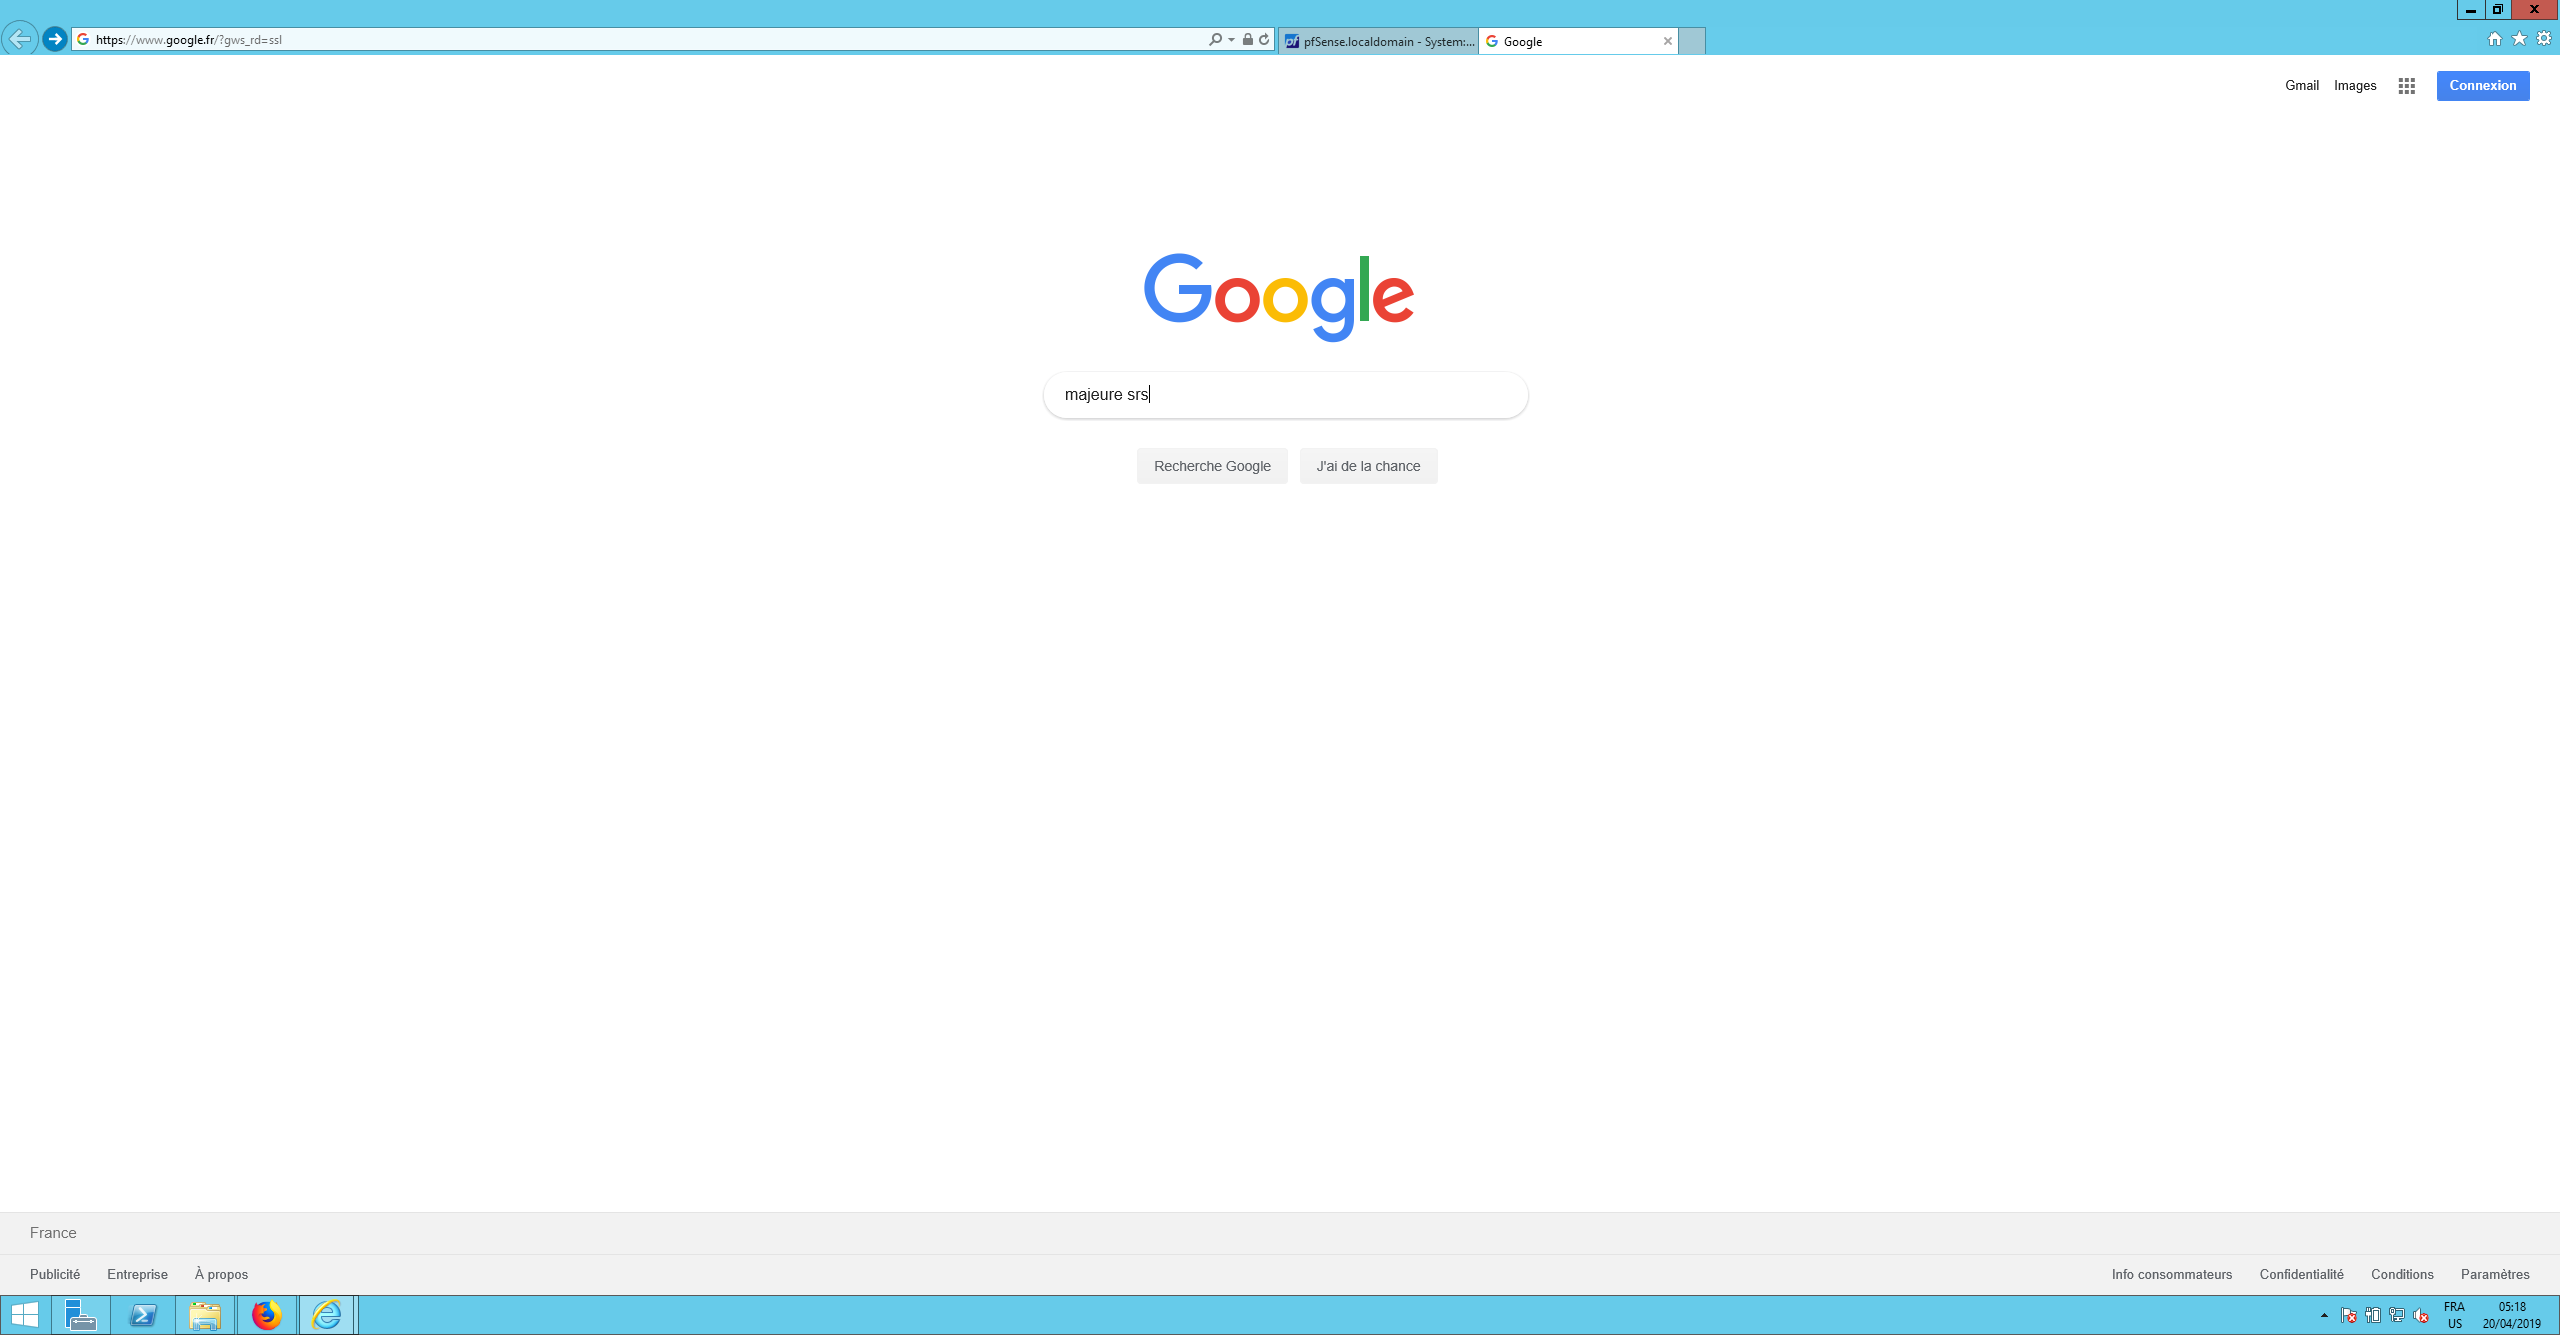
\includegraphics[scale=0.20]{Interception_Screenshots/clamAV01.png}
        \label{Pfsense_Screeshots/interception/18}
        \caption{Recherche google sans EPITA avec le filtrage clamAV}
    \end{center}
\end{figure}
\FloatBarrier

\begin{figure}[h!]
    \begin{center}
        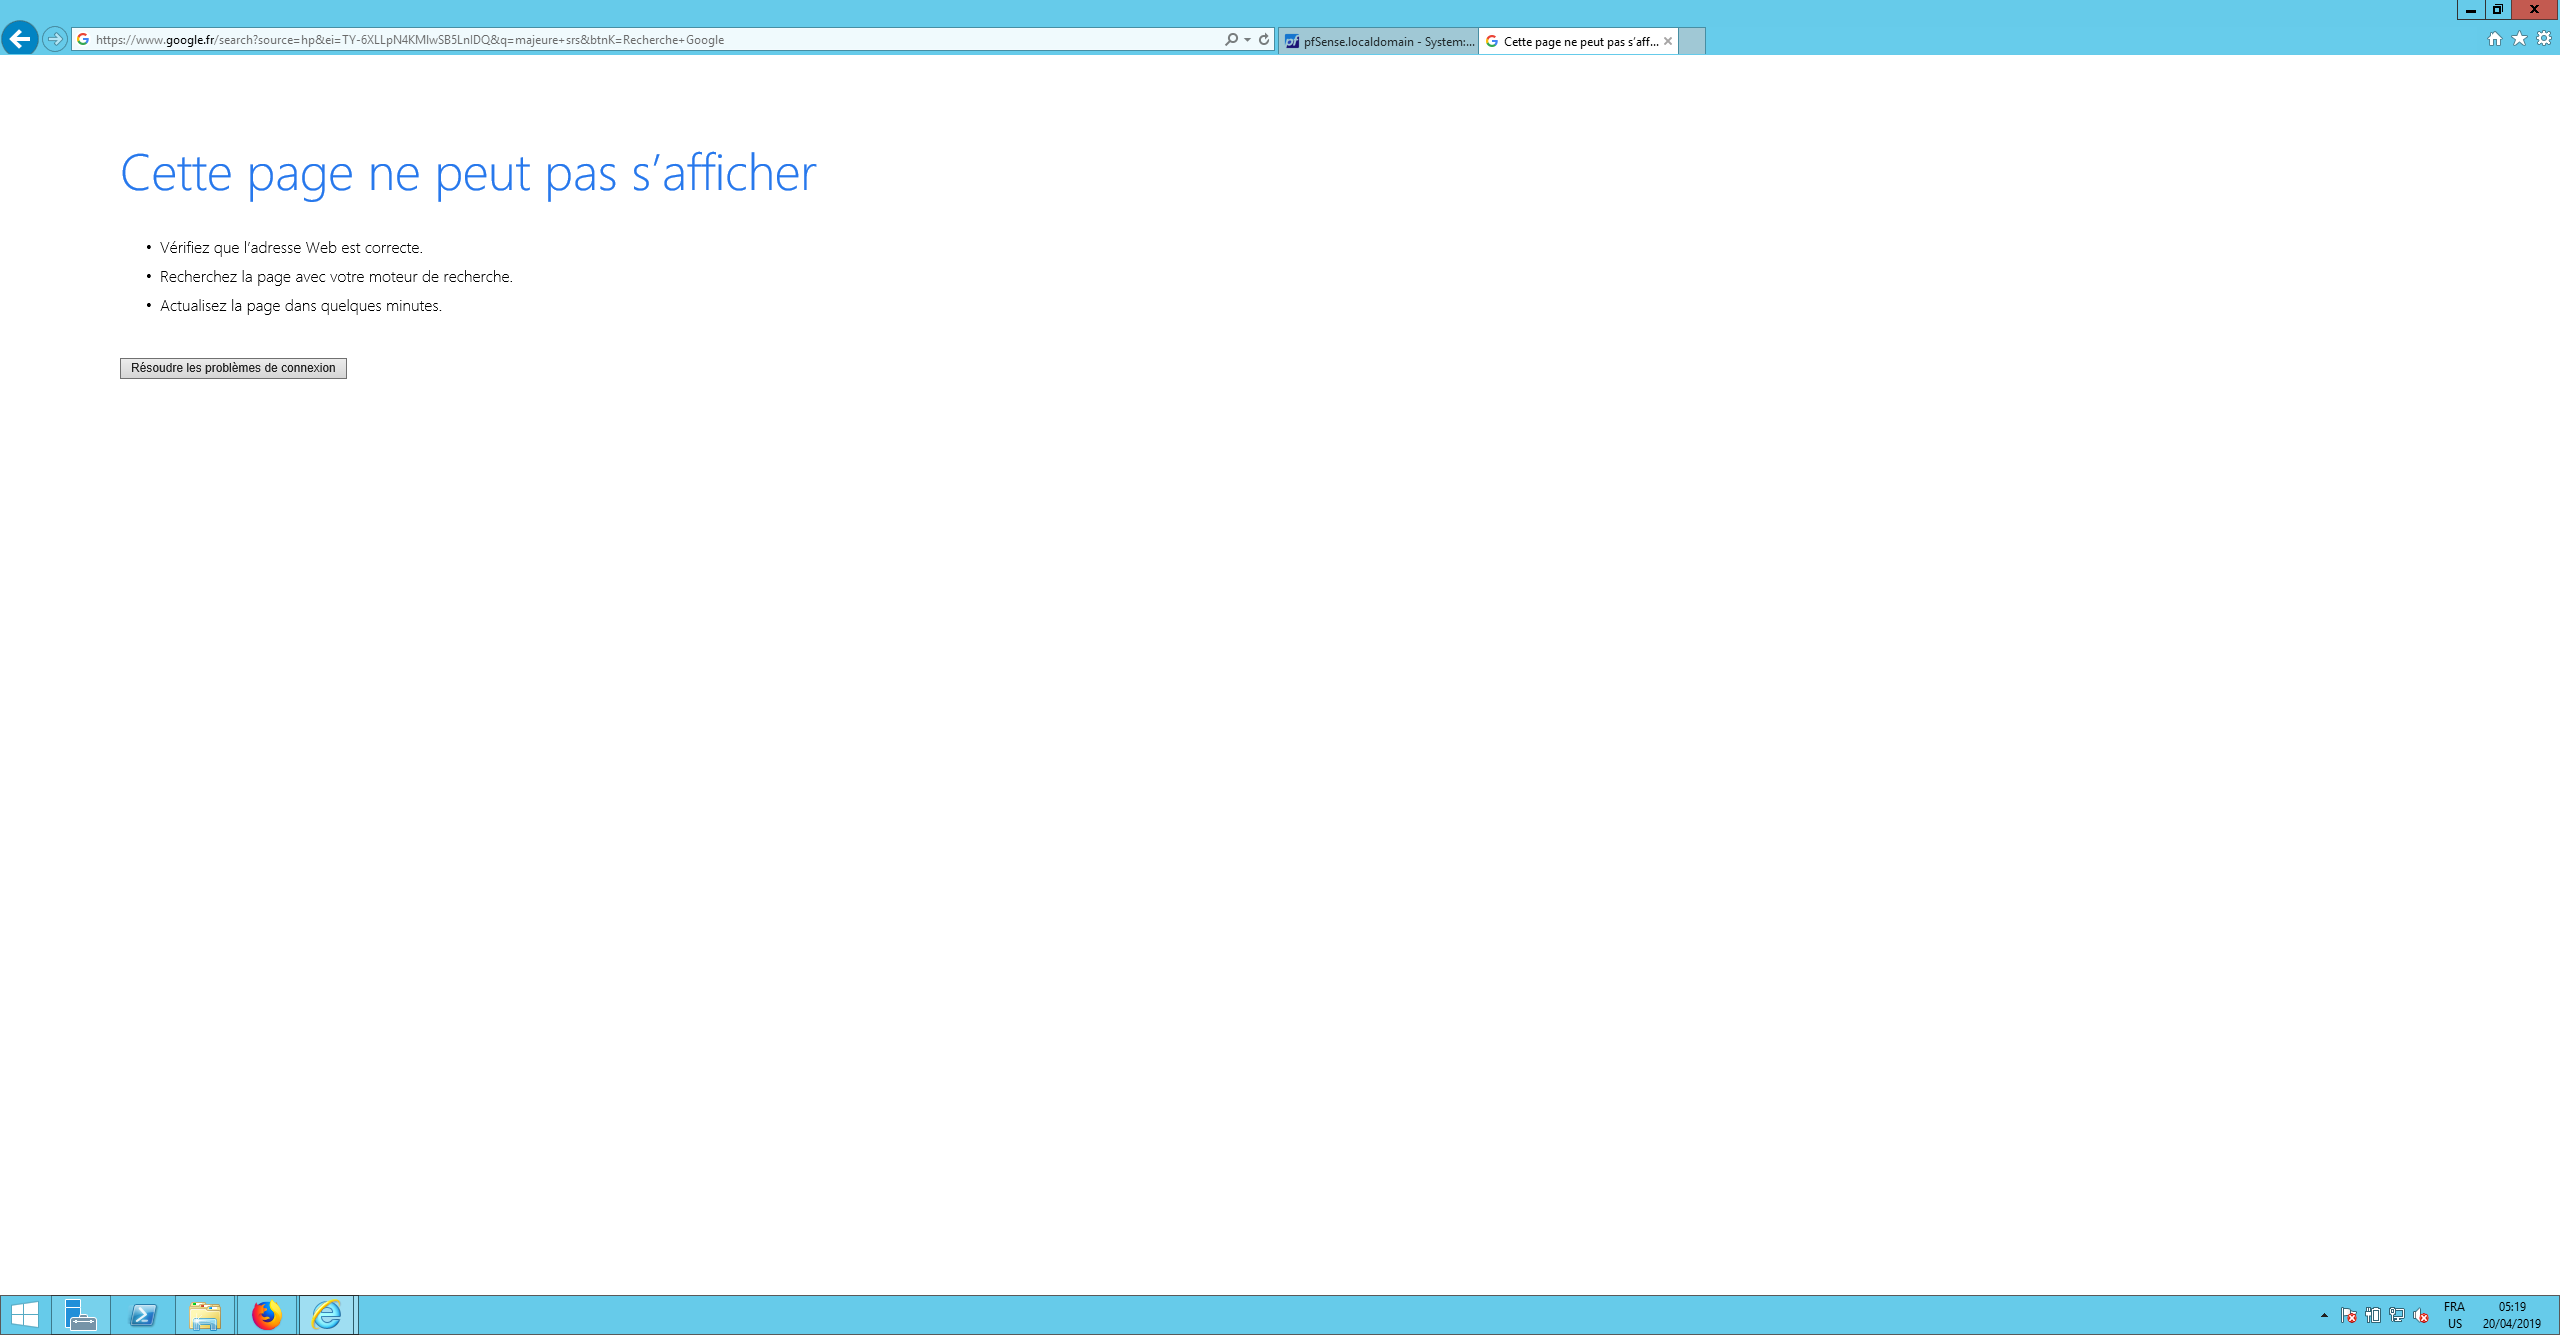
\includegraphics[scale=0.20]{Interception_Screenshots/clamAV02.png}
        \label{Pfsense_Screeshots/interception/18}
        \caption{Détection de EPITA avec le filtrage clamAV}
    \end{center}
\end{figure}
\FloatBarrier

Ce qui nous donne dans les logs :
\begin{figure}[h!]
    \begin{center}
        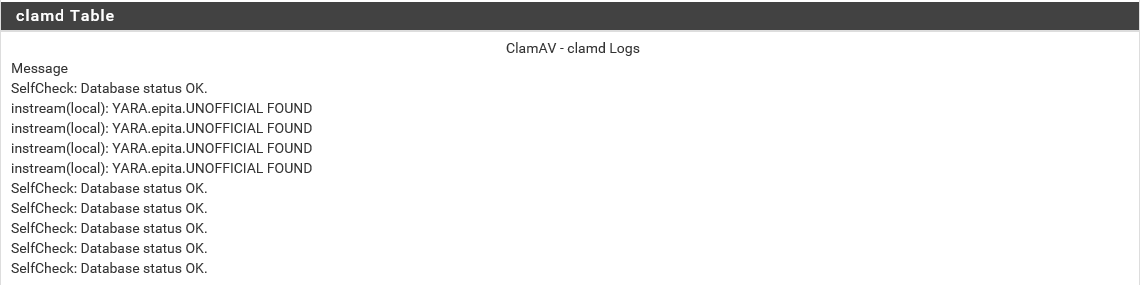
\includegraphics[scale=0.4]{Interception_Screenshots/clamAV03.png}
        \label{Pfsense_Screeshots/interception/18}
        \caption{Logs avec EPITA trouvé avec le filtrage ClamAV}
    \end{center}
\end{figure}
\FloatBarrier 